\renewcommand{\figurename}{\textbf{\suppOrApp \Fig}}
\renewcommand{\tablename}{\textbf{\suppOrApp Table}}

\begin{figure}
\section{Supporting figures}
\centering
\begin{tabular}{cc}
  \begin{subfigure}[b]{0.5\textwidth}
  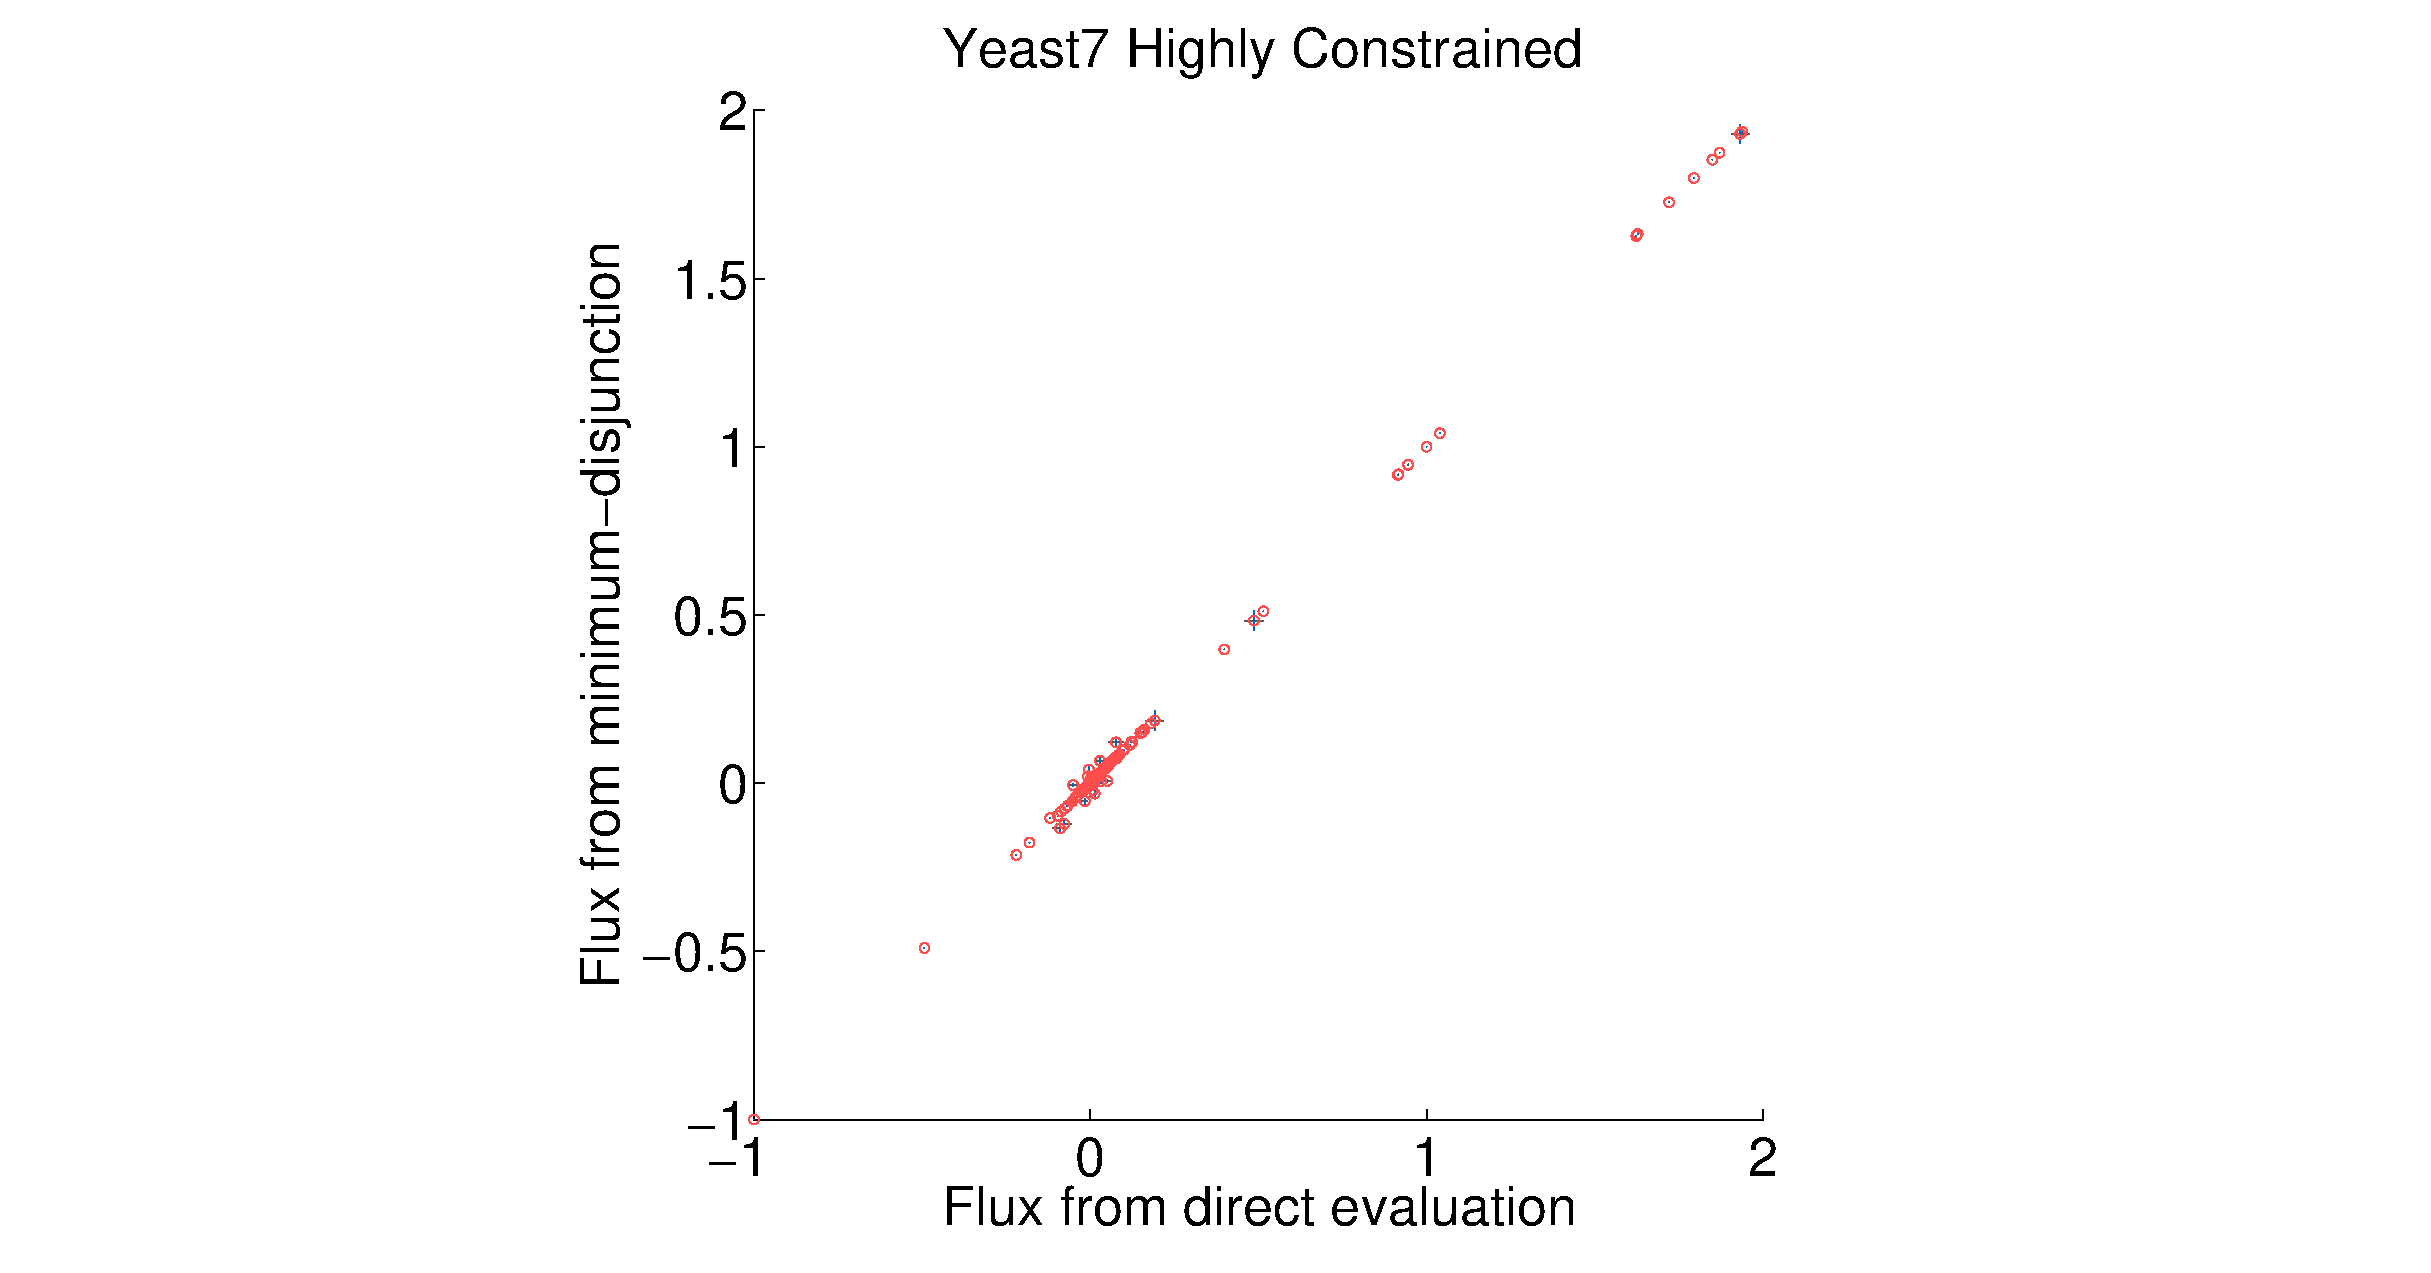
\includegraphics[width=\textwidth, trim=9cm 0cm 9cm 0cm, clip=true]
  {expCmpY7HC}
  \caption{highly constrained} \label{fig:EnzAbundEval:A}
  \end{subfigure}
&
  \begin{subfigure}[b]{0.5\textwidth}
  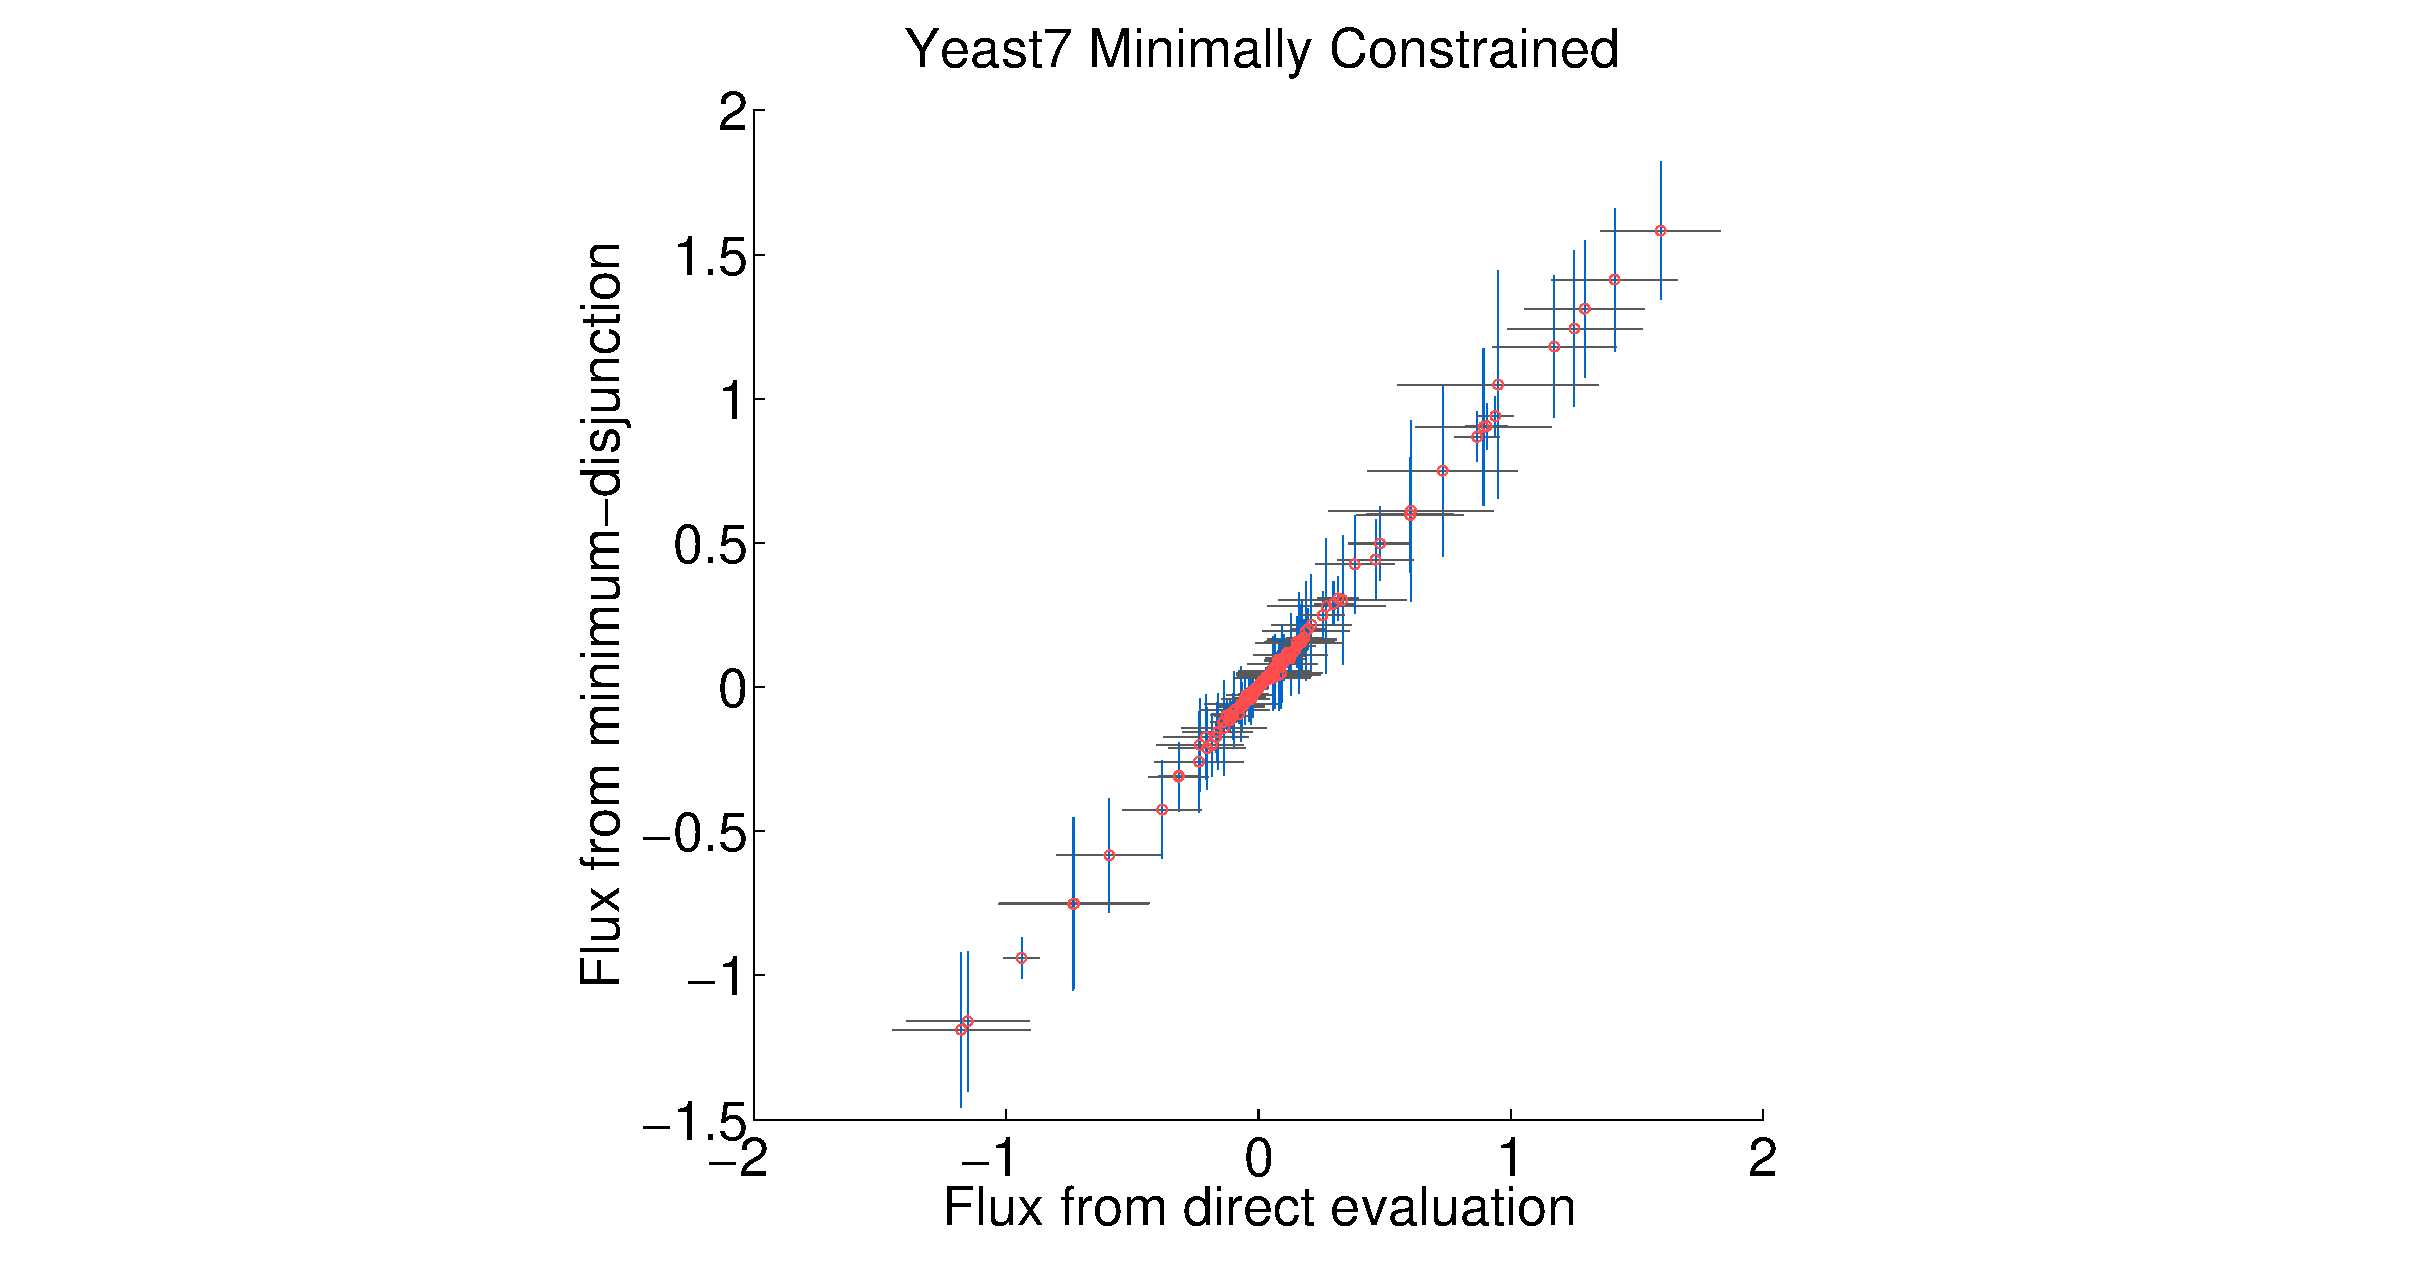
\includegraphics[width=\textwidth, trim=9cm 0cm 9cm 0cm, clip=true]
  {expCmpY7MC}
  \caption{minimally constrained} \label{fig:EnzAbundEval:B}
  \end{subfigure} 
\\
  \begin{subfigure}[b]{0.5\textwidth}
  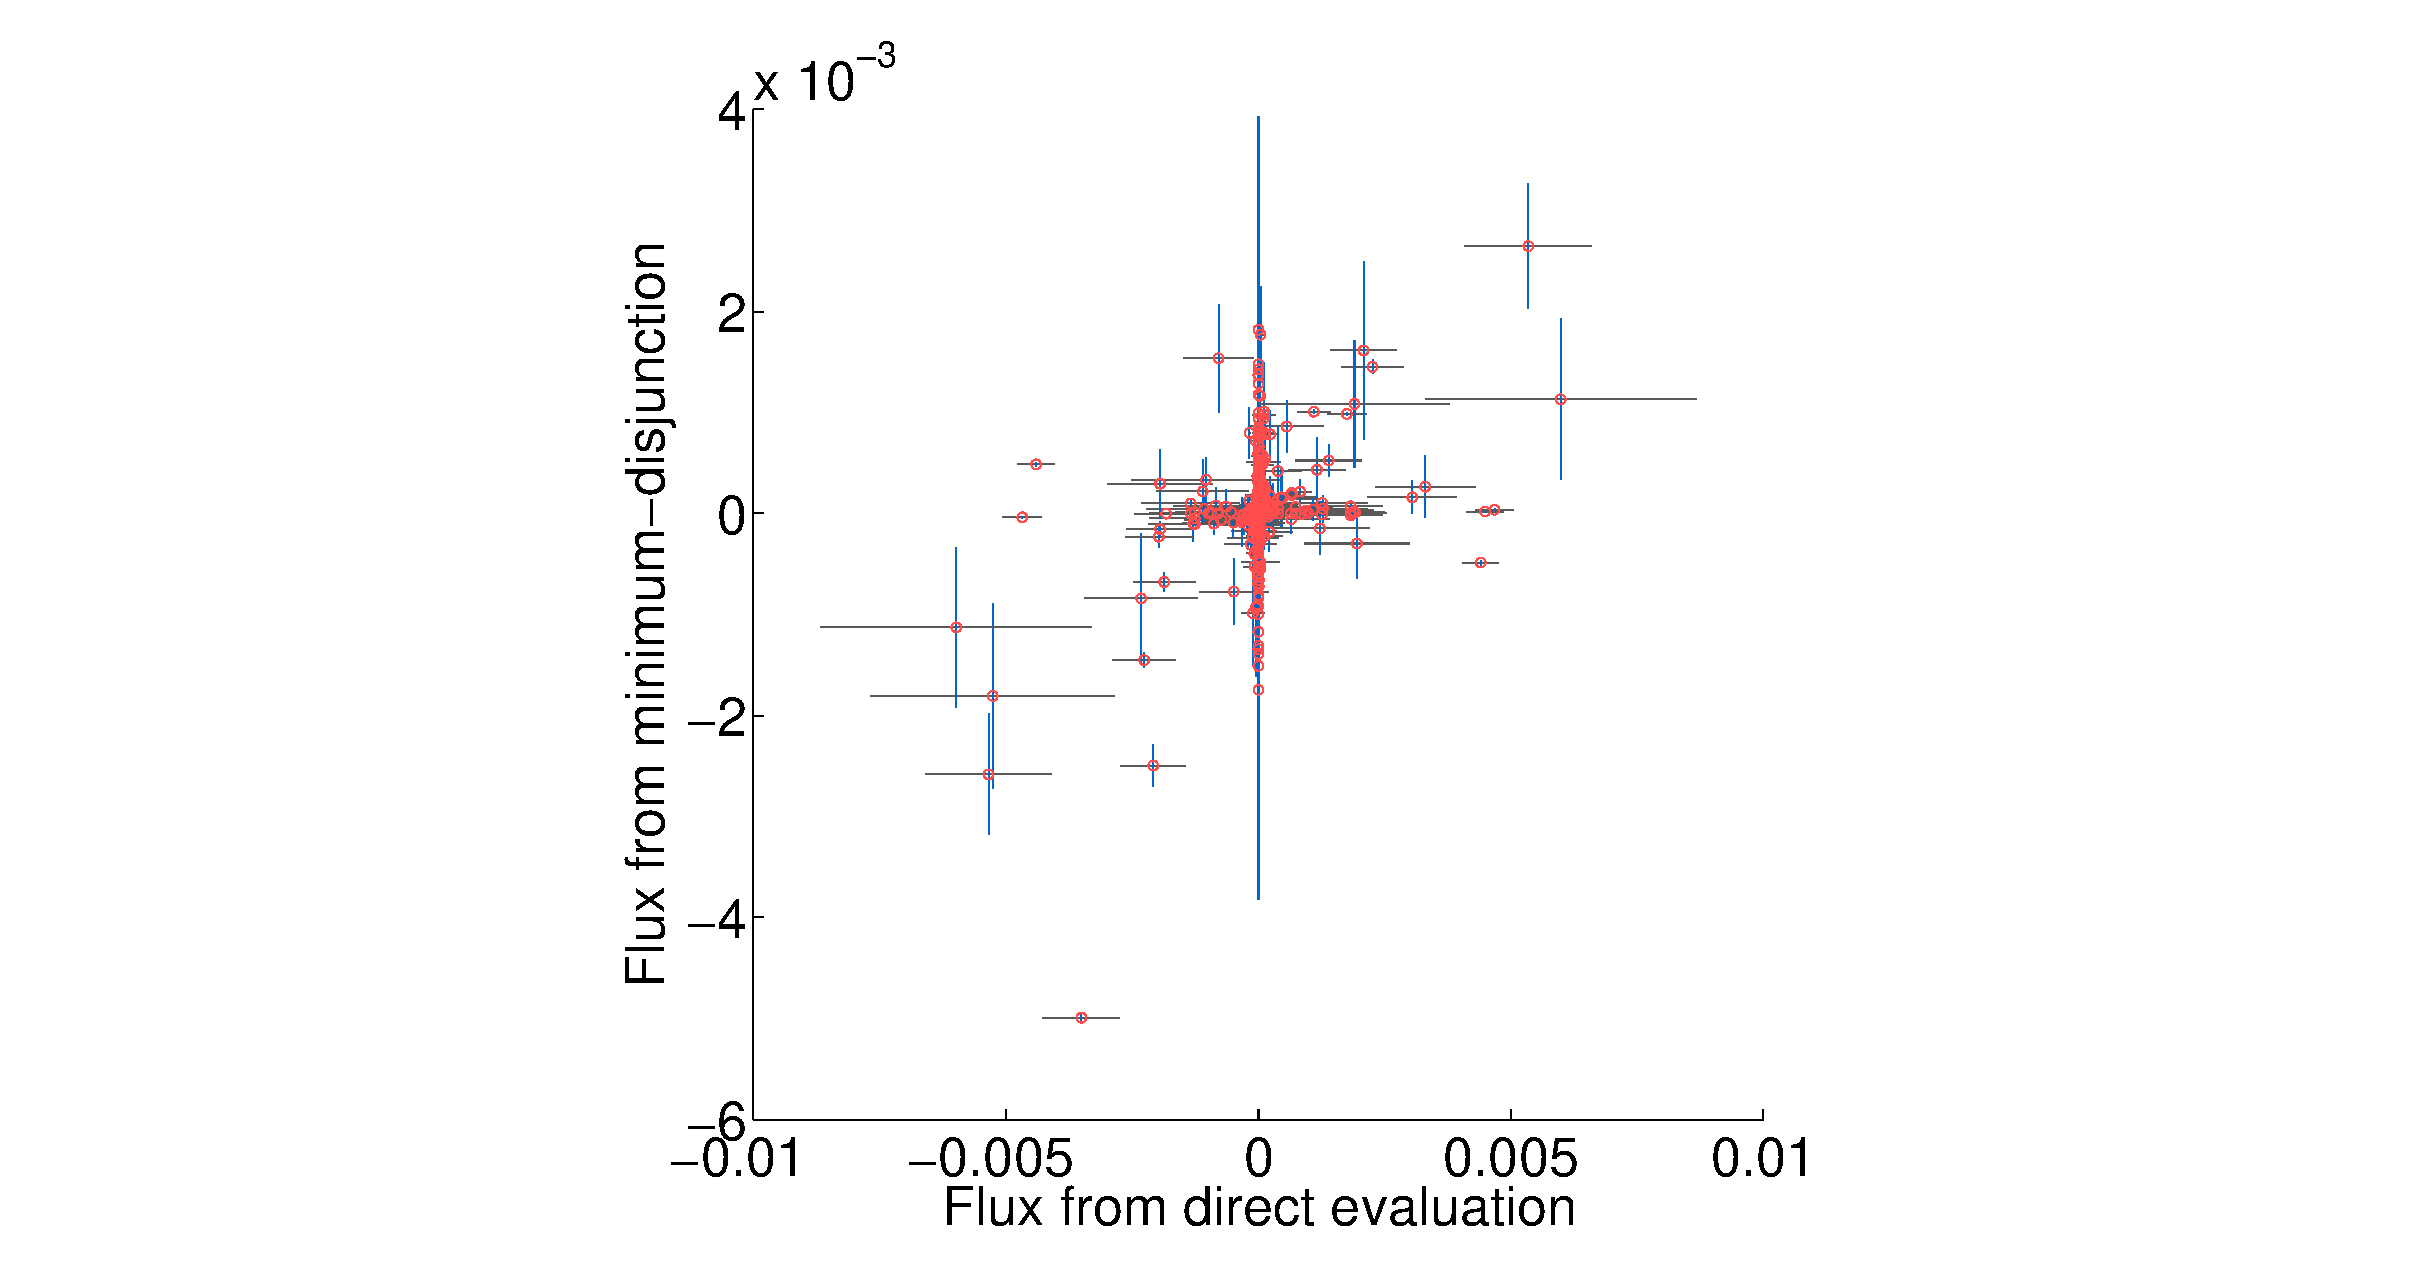
\includegraphics[width=\textwidth, trim=9cm 0cm 9cm 0cm, clip=true]
  {expCmpR2HC}
  \caption{highly constrained} \label{fig:EnzAbundEval:C}
  \end{subfigure}
&
  \begin{subfigure}[b]{0.5\textwidth}
  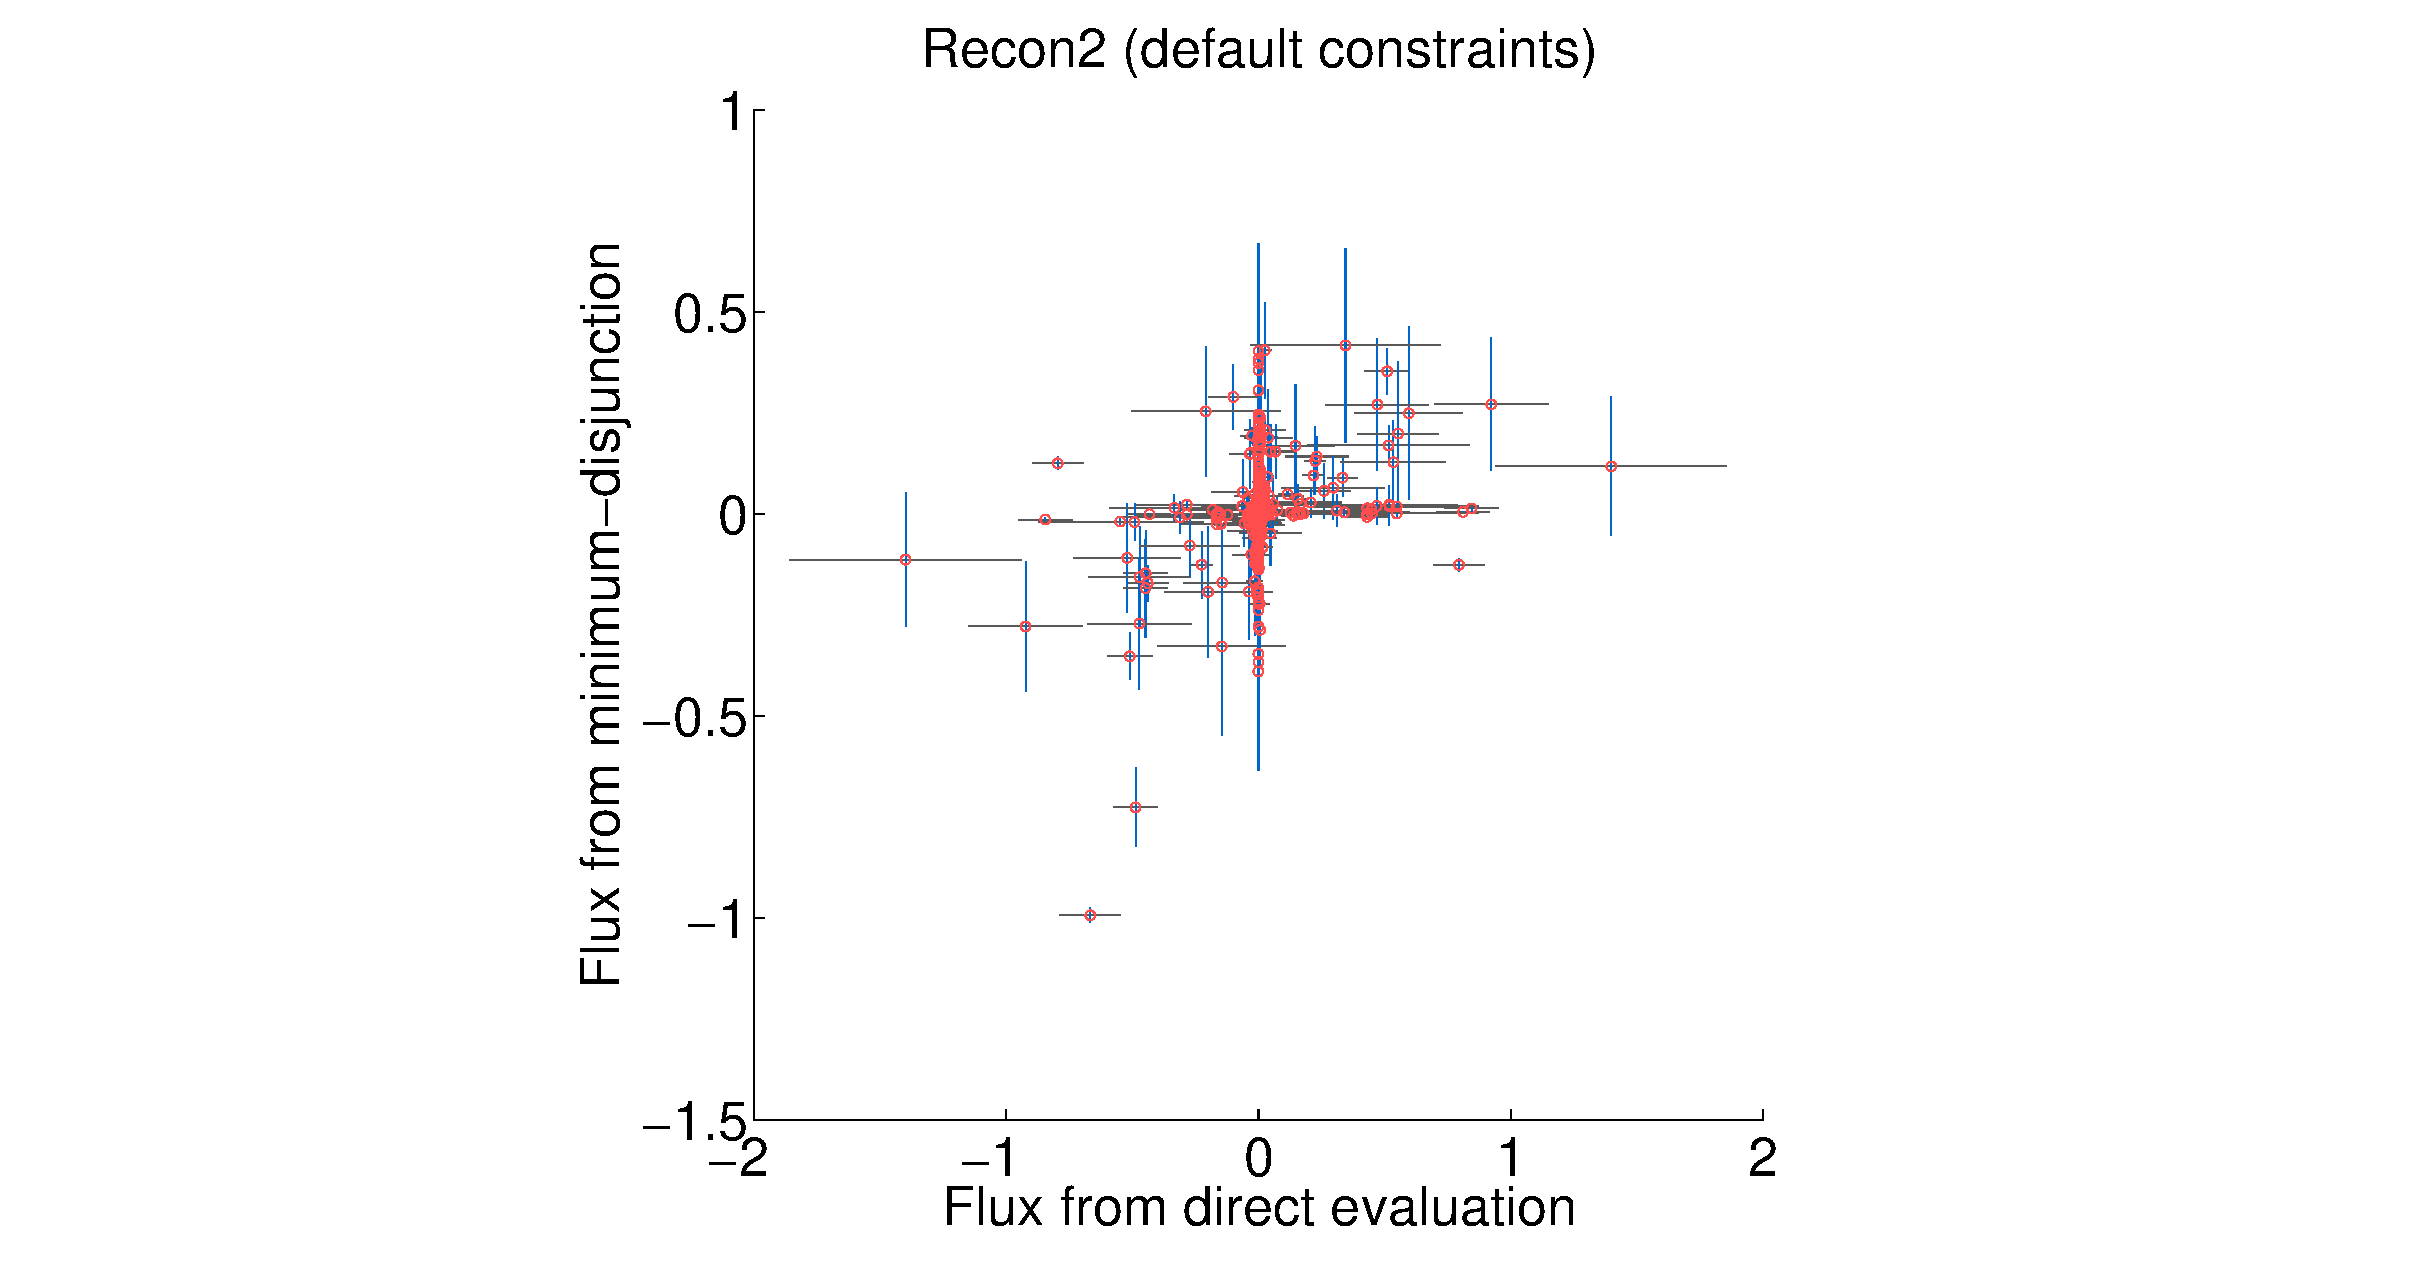
\includegraphics[width=\textwidth, trim=9cm 0cm 9cm 0cm, clip=true]
  {expCmpR2dC}
  \caption{minimally constrained} \label{fig:EnzAbundEval:D}
  \end{subfigure} 
\\
\end{tabular}
\caption{Comparison of fluxes when FALCON is run with enzyme abundance
calculated by direct evaluation (x-axis) and the minimum disjunction
algorithm (y-axis); error bars with length equal to one standard
deviation are shown for both approaches as a result of alternative
solutions in FALCON. Yeast was evaluated with default (highly)
constrained \textbf{(a)} and minimally constrained \textbf{(b)}
models, and no strong difference between direct evaluation or or the
minimum disjunction method is observed in either case. However, for
human models with a highly constrained reaction set (RPMI media,
CORE-sign, and enzymatic direction) \textbf{(c)} and default
constraints \textbf{(d)}, we see there is a large amount of variation
between the two evaluation techniques. In the human cases, two
outliers were not shown that correspond to a single large flux cycle
(`release of B12 by simple diffusion' and `transport of
Adenosylcobalamin into the intestine').}
\label{fig:EnzAbundEval}
\end{figure}
\FloatBarrier


\begin{figure}[!htb]
\begin{tabular}{cc}
  \begin{subfigure}[b]{0.48\textwidth}
  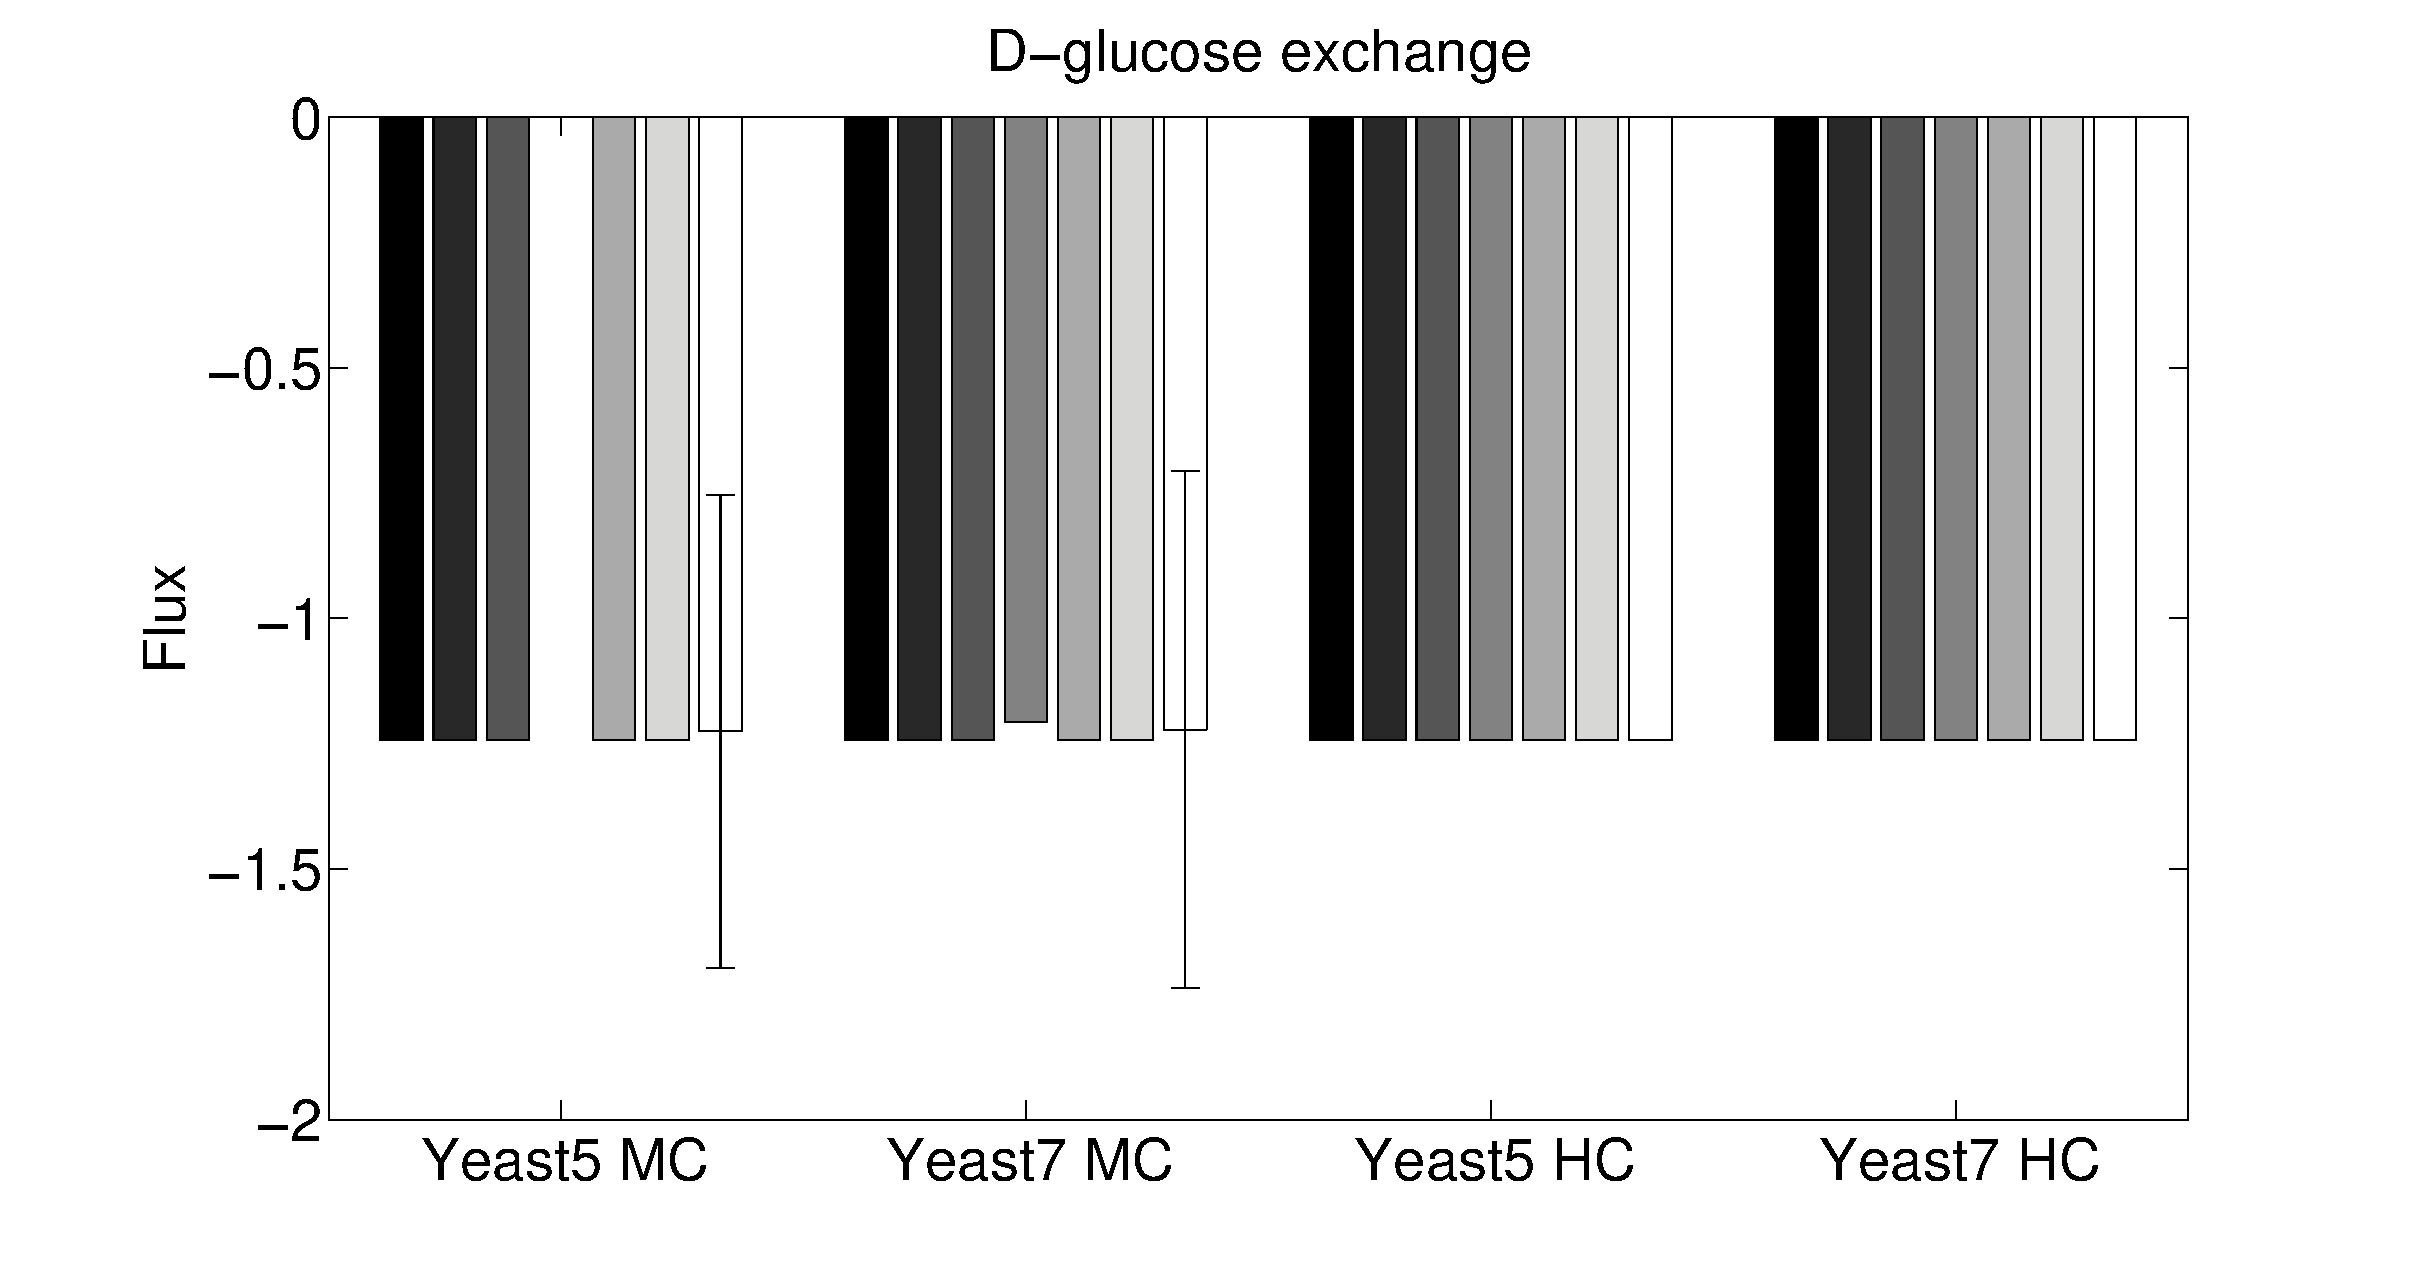
\includegraphics[width=\textwidth]{gluc75_bars}
  \caption{glucose}
  \end{subfigure}
&
  \begin{subfigure}[b]{0.48\textwidth}
  \raisebox{0.3\height}{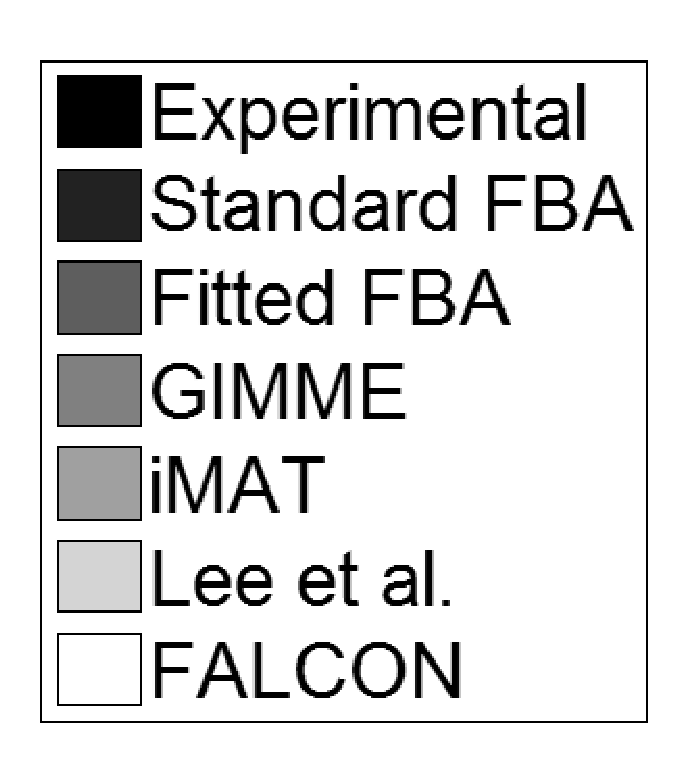
\includegraphics[scale=0.4,center]{legend_bars}}
%  [width=\textwidth, trim=9cm 4cm 5cm 1cm, clip=true]{legend_bars}}
  \end{subfigure} 
\\
  \begin{subfigure}[b]{0.48\textwidth}
  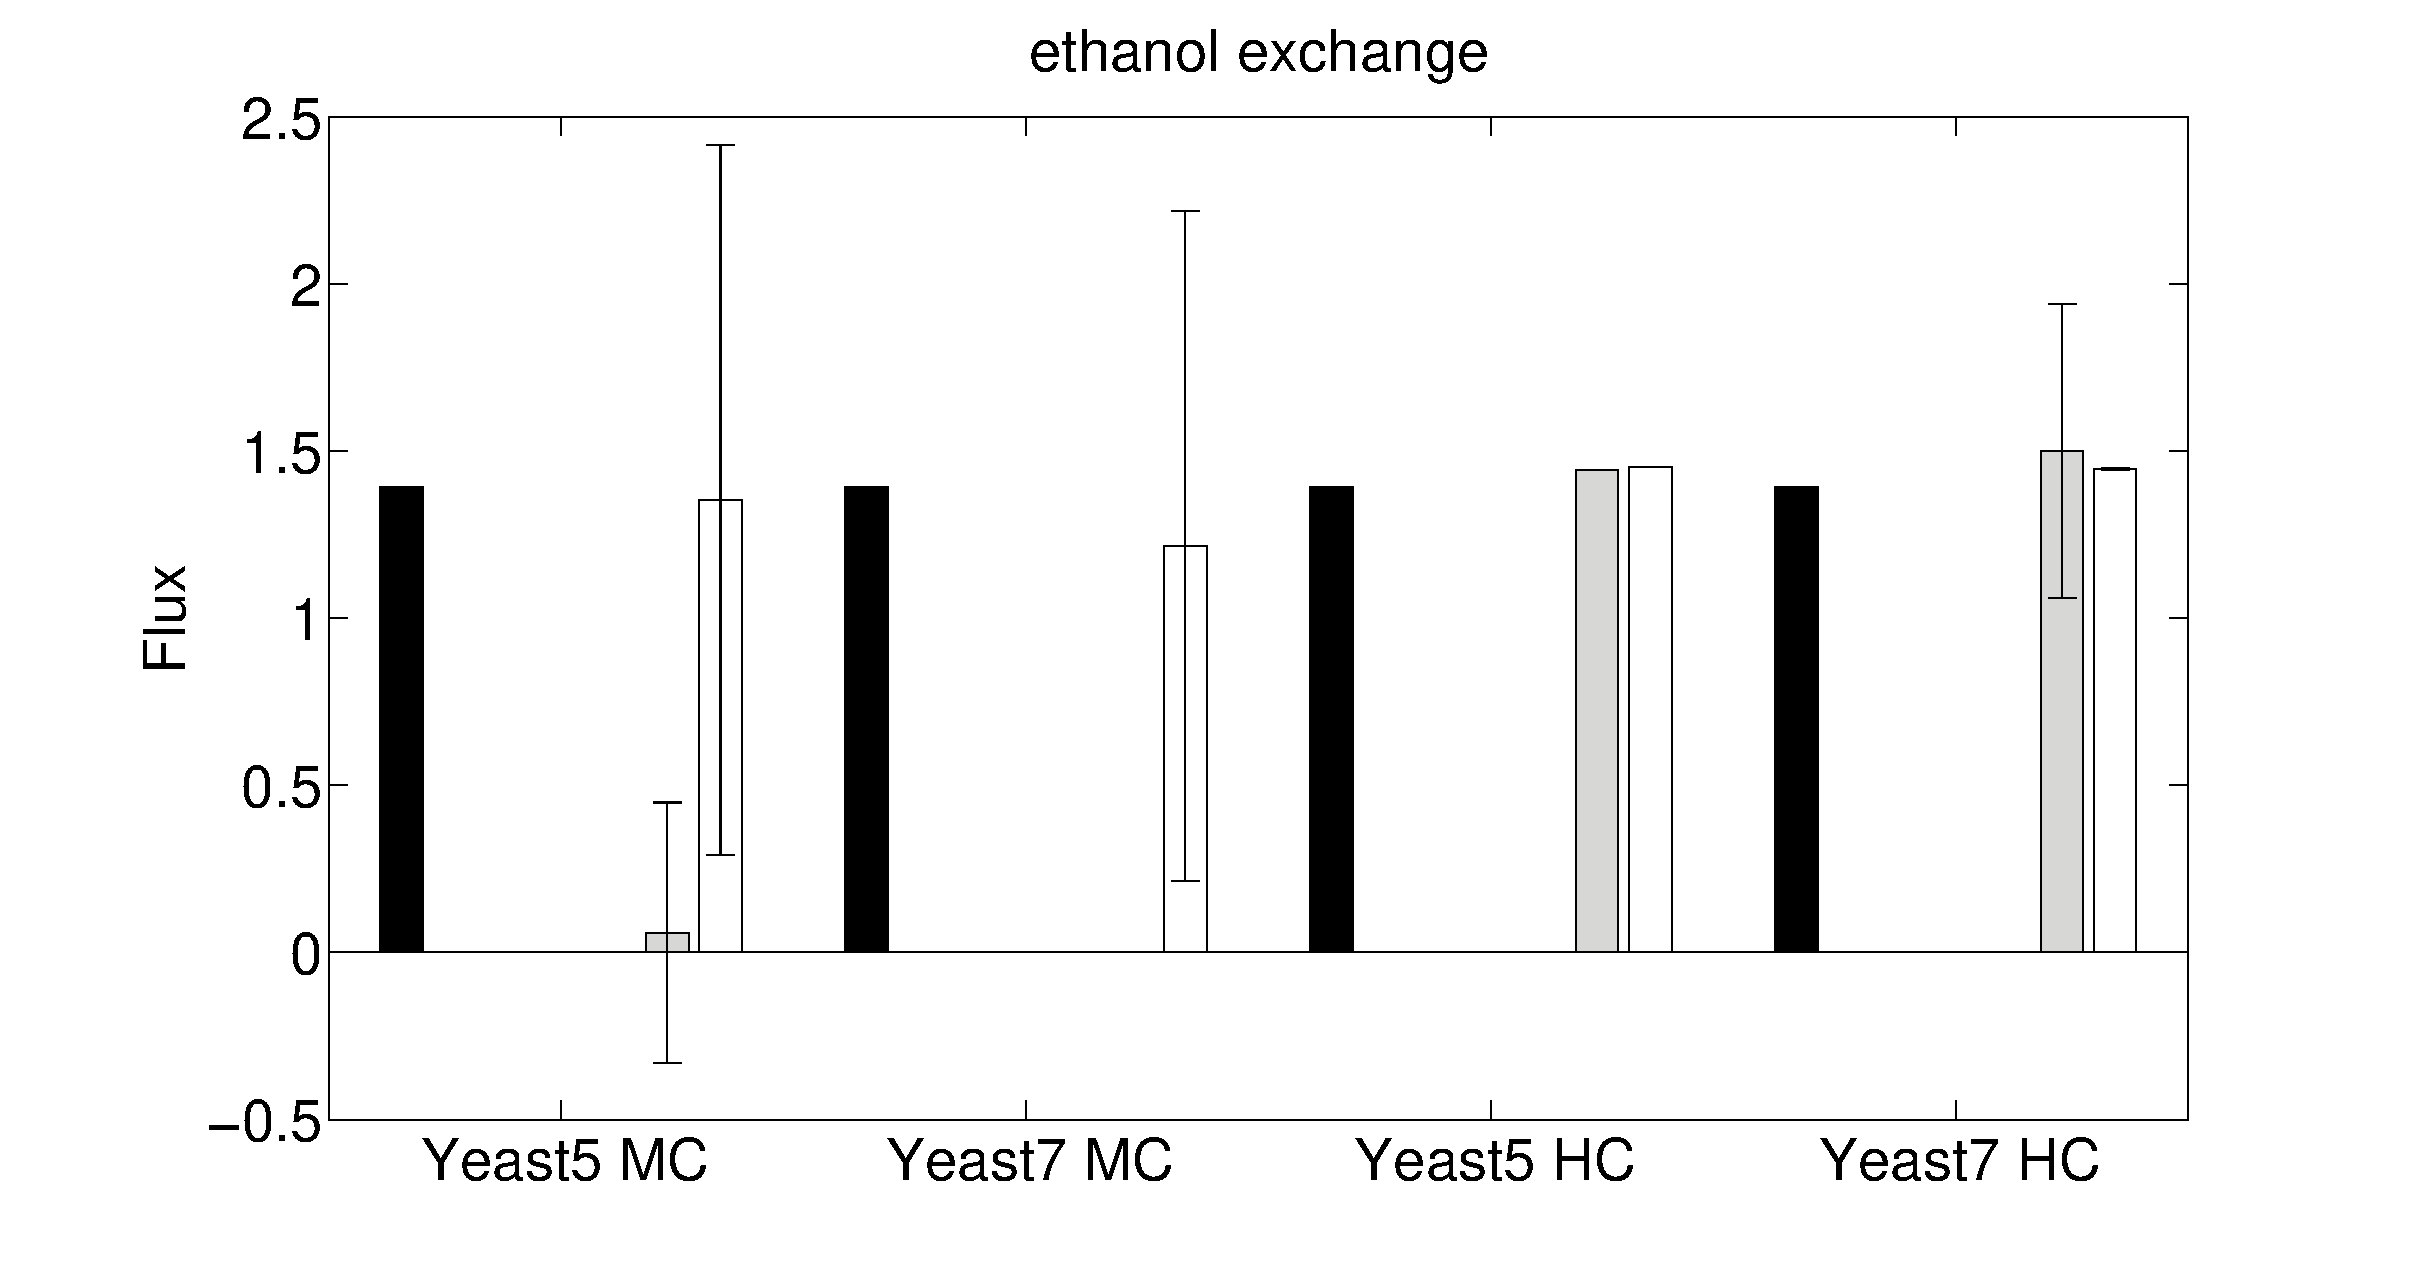
\includegraphics[width=\textwidth]{eth75_bars}
  \caption{ethanol}
  \end{subfigure} 
&
  \begin{subfigure}[b]{0.48\textwidth}
  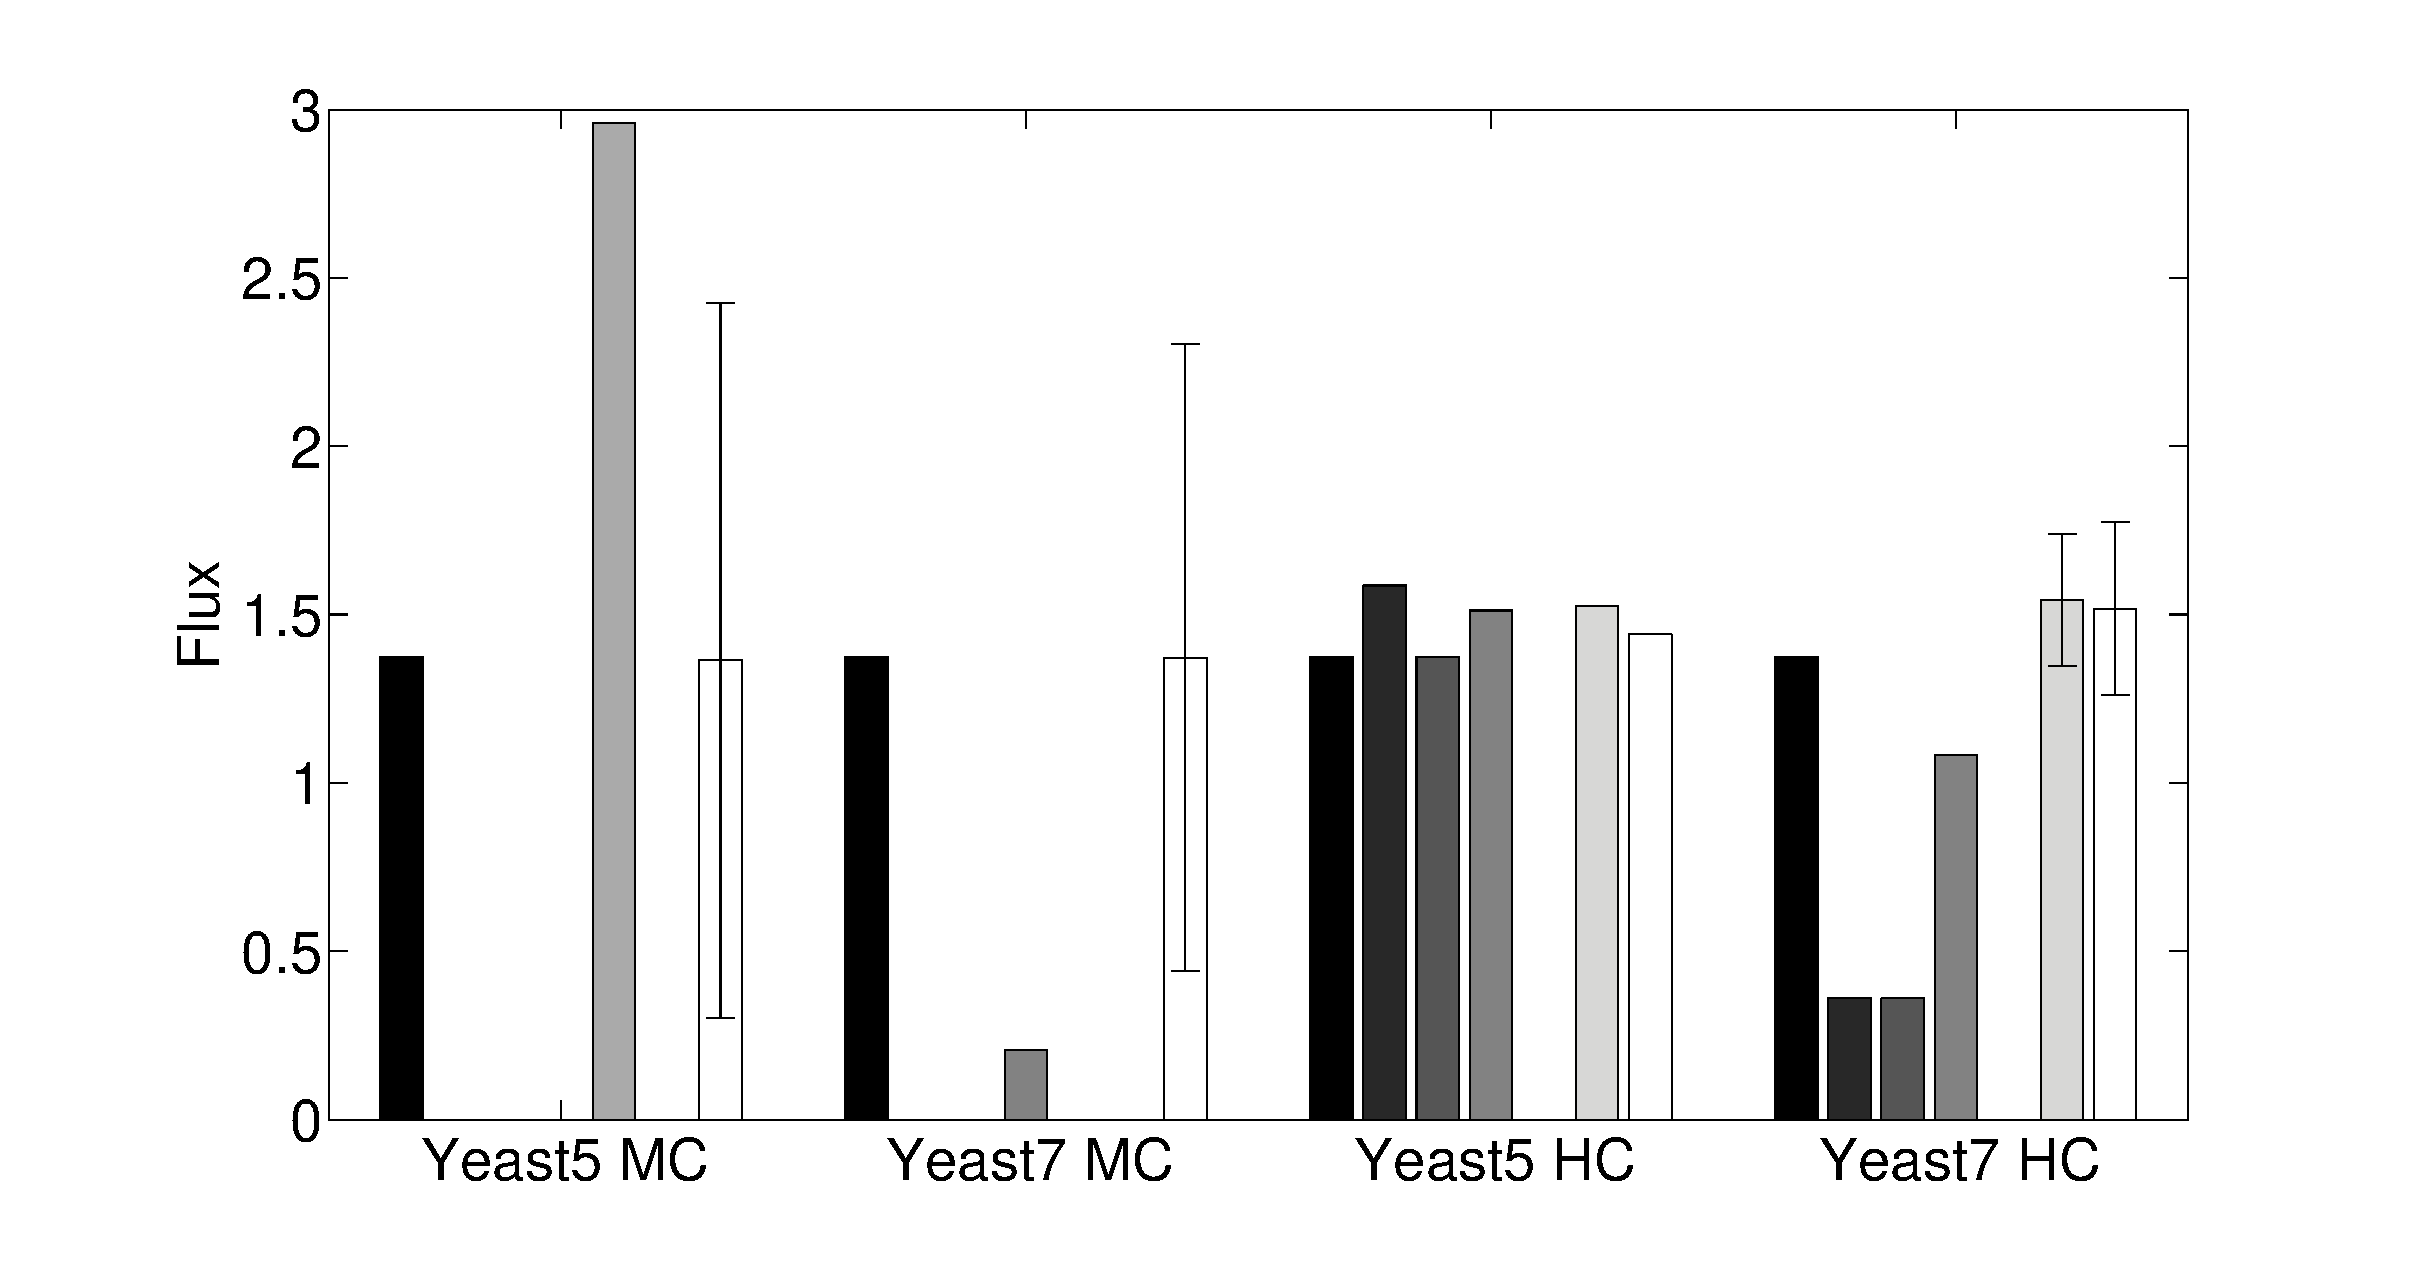
\includegraphics[width=\textwidth]{co2_75_bars}
  \caption{CO$_2$}
  \end{subfigure} 
\\
  \begin{subfigure}[b]{0.48\textwidth}
  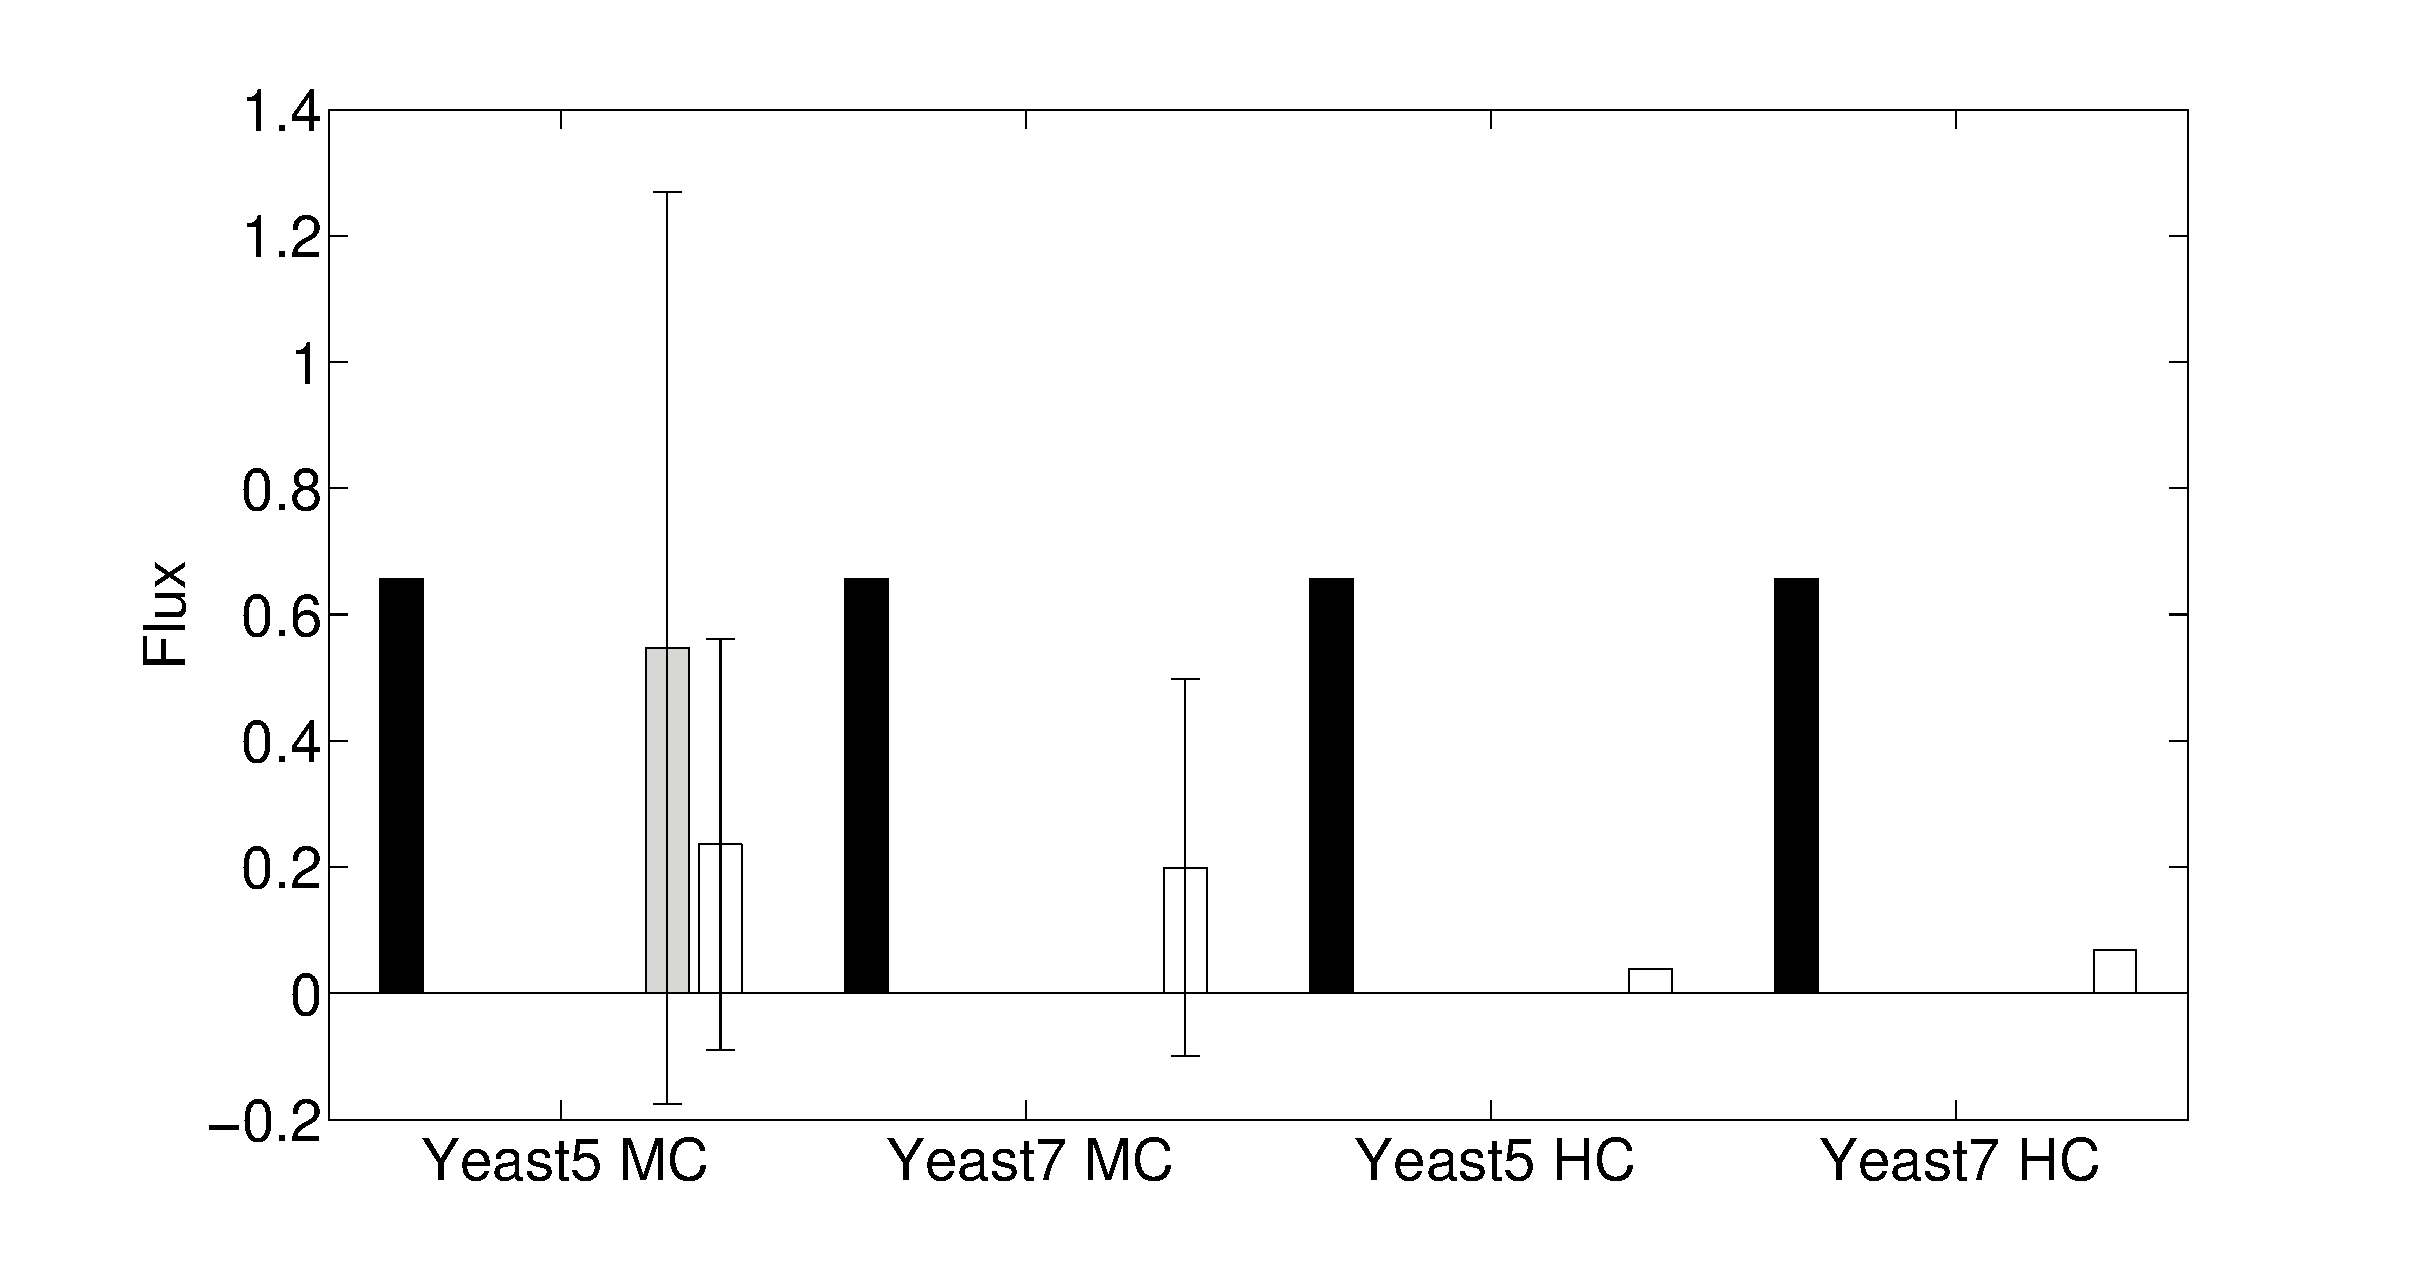
\includegraphics[width=\textwidth]{glycerol75_bars}
  \caption{glycerol}
  \end{subfigure} 
&
  \begin{subfigure}[b]{0.48\textwidth}
  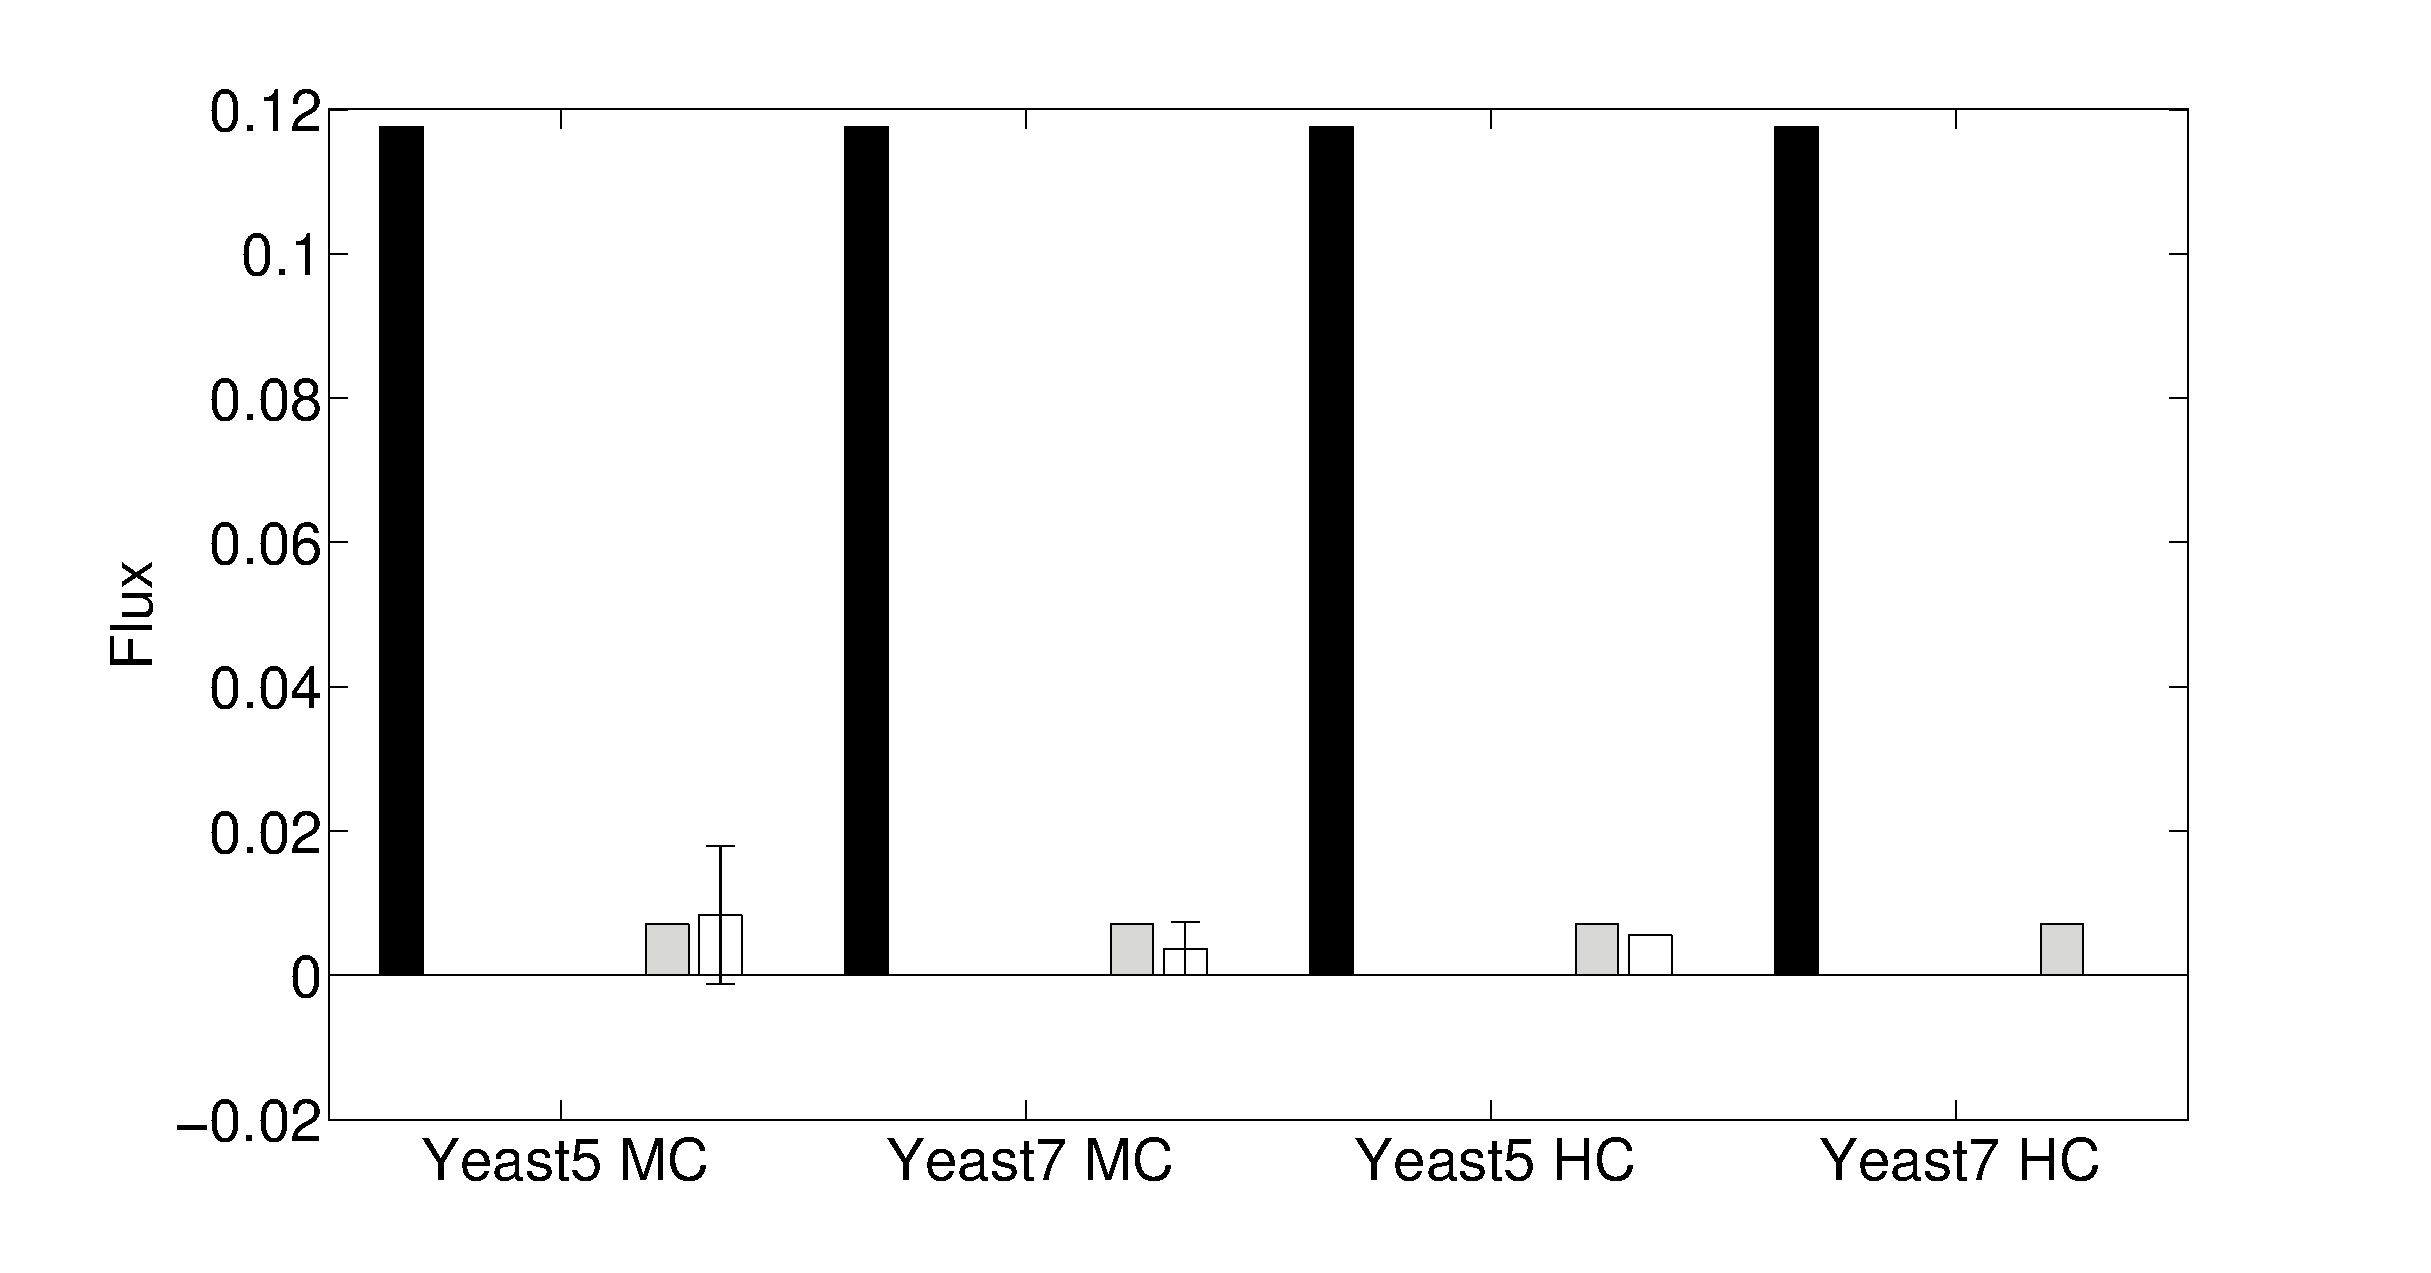
\includegraphics[width=\textwidth]{acetate75_bars}
  \caption{acetate}
  \end{subfigure} 
\\
\end{tabular}
\caption{
Shown are flux predictions using a number of methods and four
different models (Yeast~5 MC and Yeast~7 MC are minimally constrained
Yeast~5 and Yeast~7; Yeast~5 HC and Yeast~7 HC are highly constrained Yeast~5
and Yeast~7). Error bars are shown for the Lee et al. method and for
FALCON, where one side of the error bar corresponds to a standard
deviation. Note that there can be no variation for glucose in the
former case since glucose flux is fixed as part of the method. FALCON
performs very well for large fluxes \textbf{(a-c)}, and is also the best
performer in general for the next largest flux, glycerol \textbf{(d)}. It also
has sporadic success for smaller fluxes, but all methods seem to have
trouble with the smallest fluxes (e.g. \textbf{e}). Note that fluxes are drawn
in log scale (specifically a flux $v$ is drawn as $\sgn{v} \log_{10}{\left( 
1 + v\right)} $). Similar results are obtainable for the 85\% maximum growth
condition.}
\label{fig:FluxBars}
\end{figure}
\FloatBarrier

\begin{figure}[!htb]
\centering
\begin{tabular}{cc}
  \begin{subfigure}[b]{0.5\textwidth}
  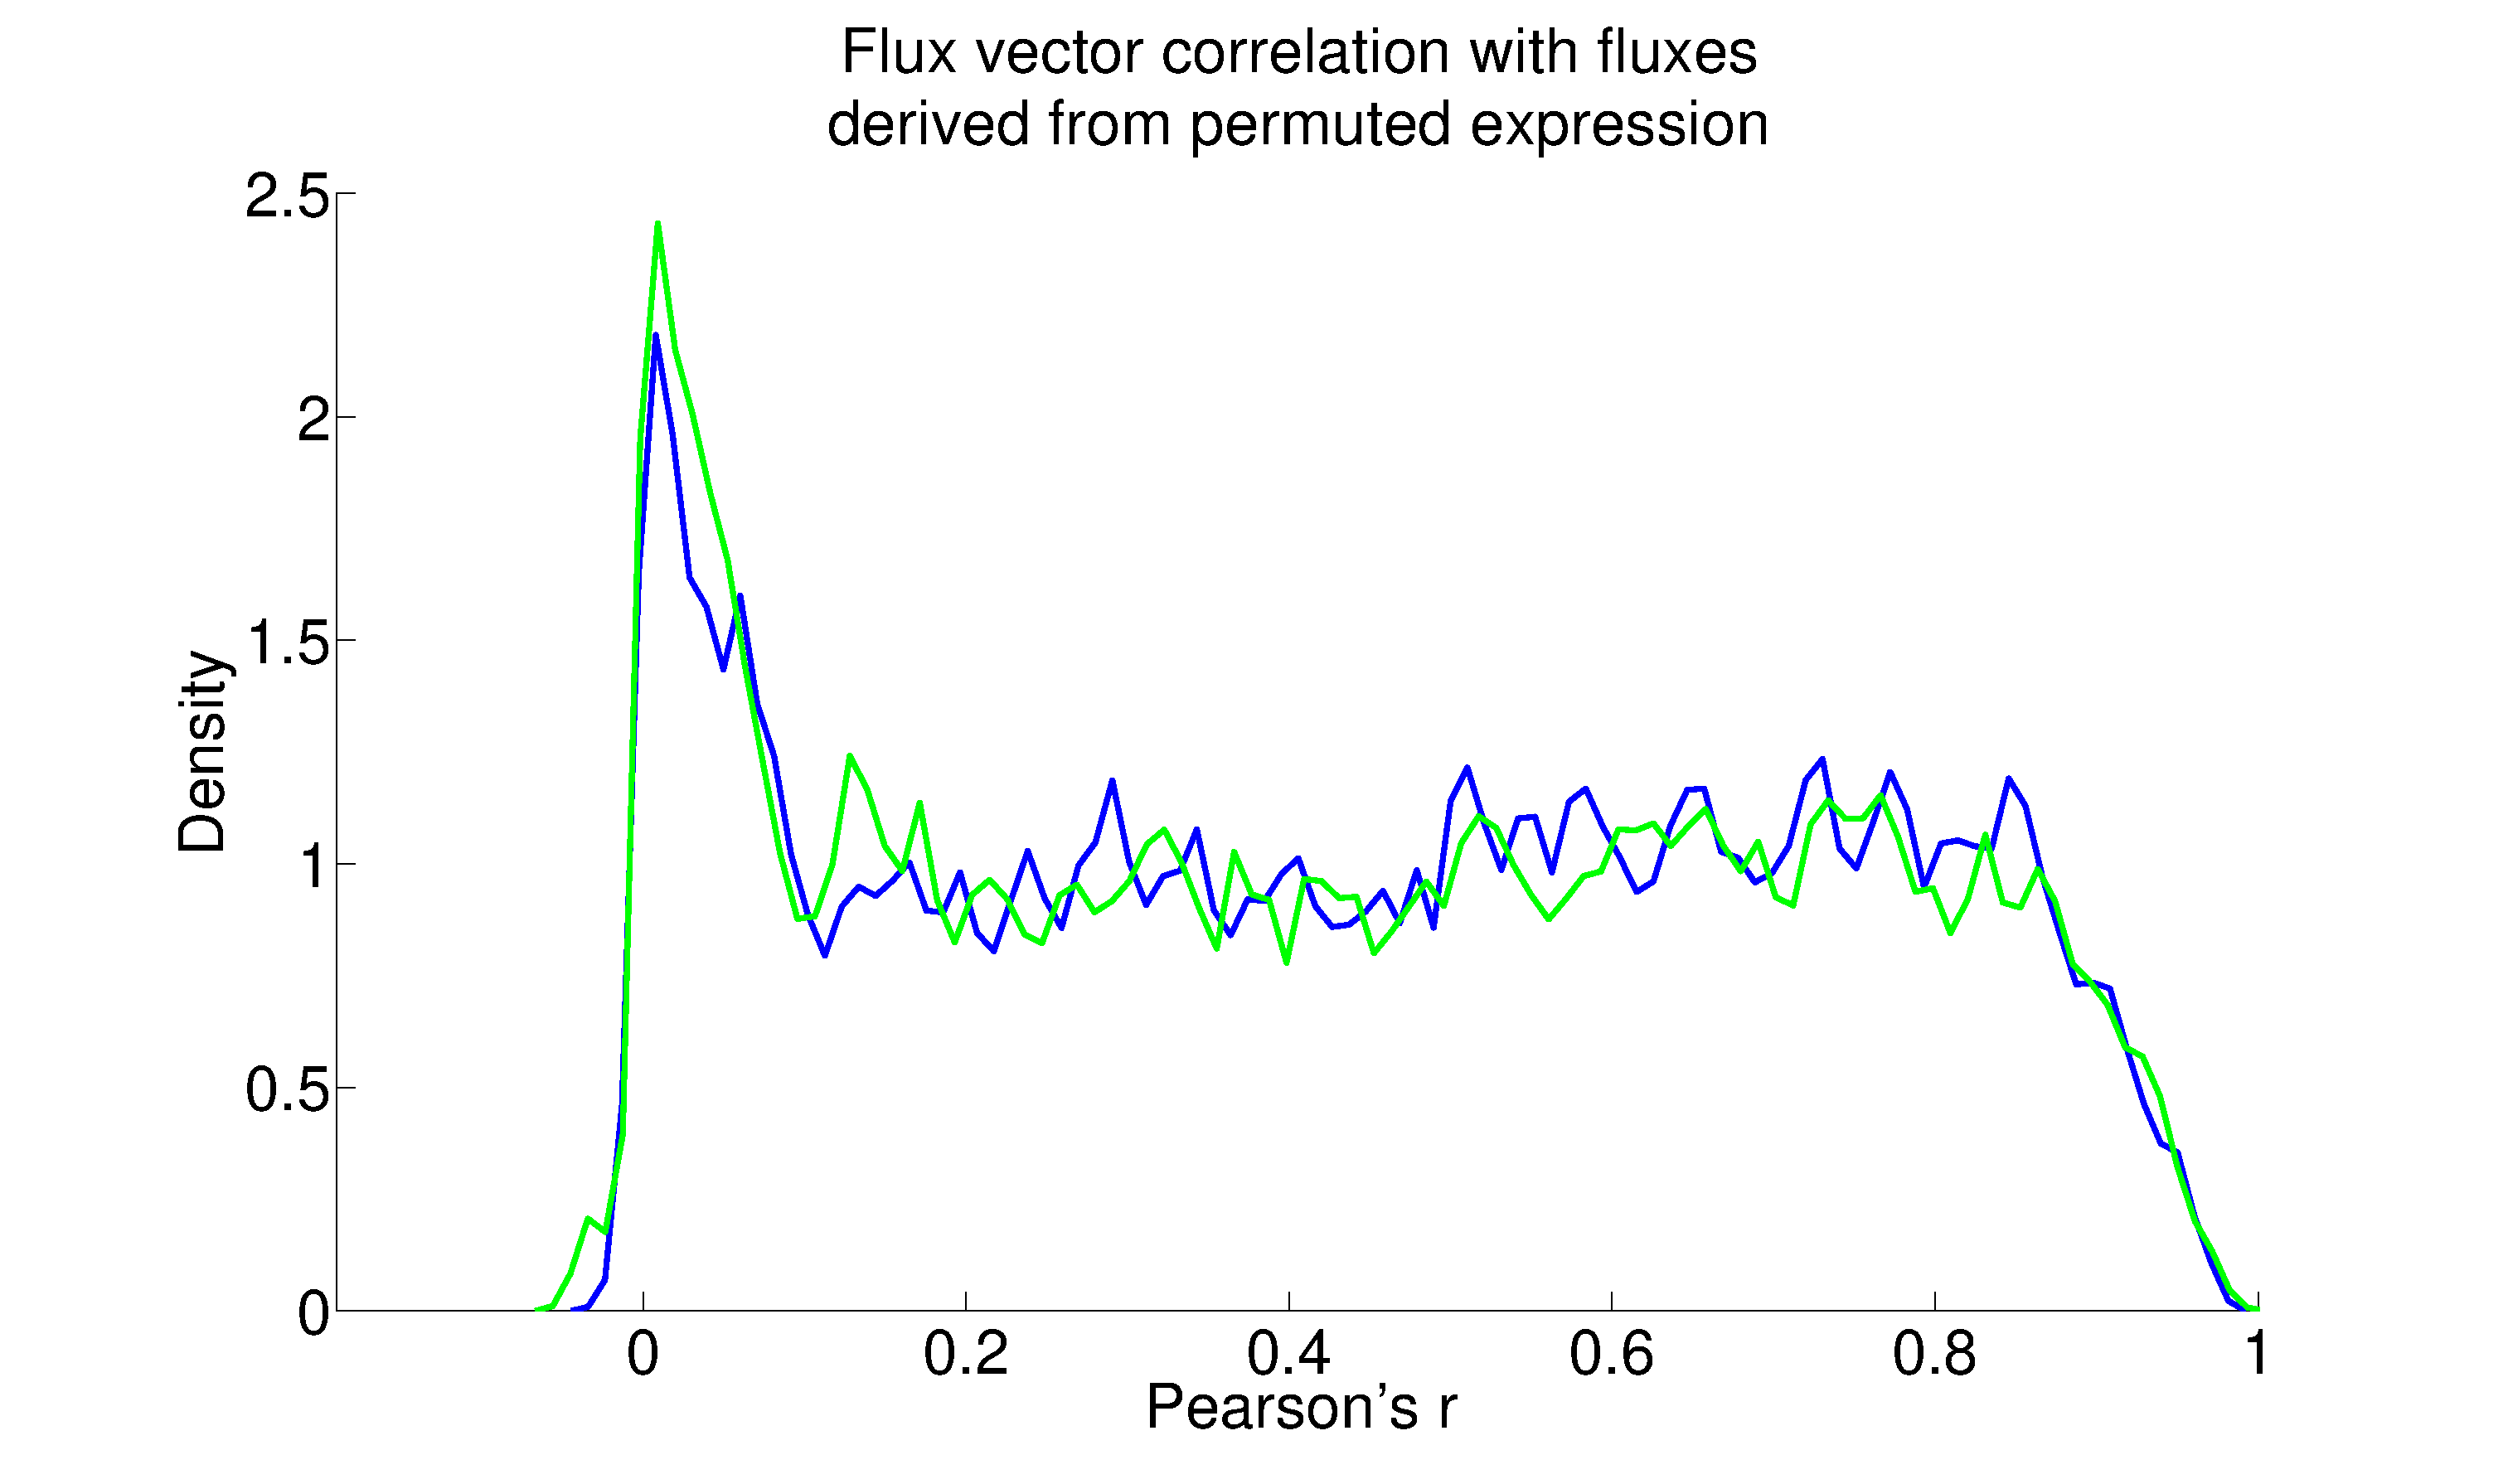
\includegraphics[width=\textwidth]{pFluxVec}
  \caption{highly constrained} \label{fig:YpermCorrSup:A}
  \end{subfigure}
&
  \begin{subfigure}[b]{0.5\textwidth}
  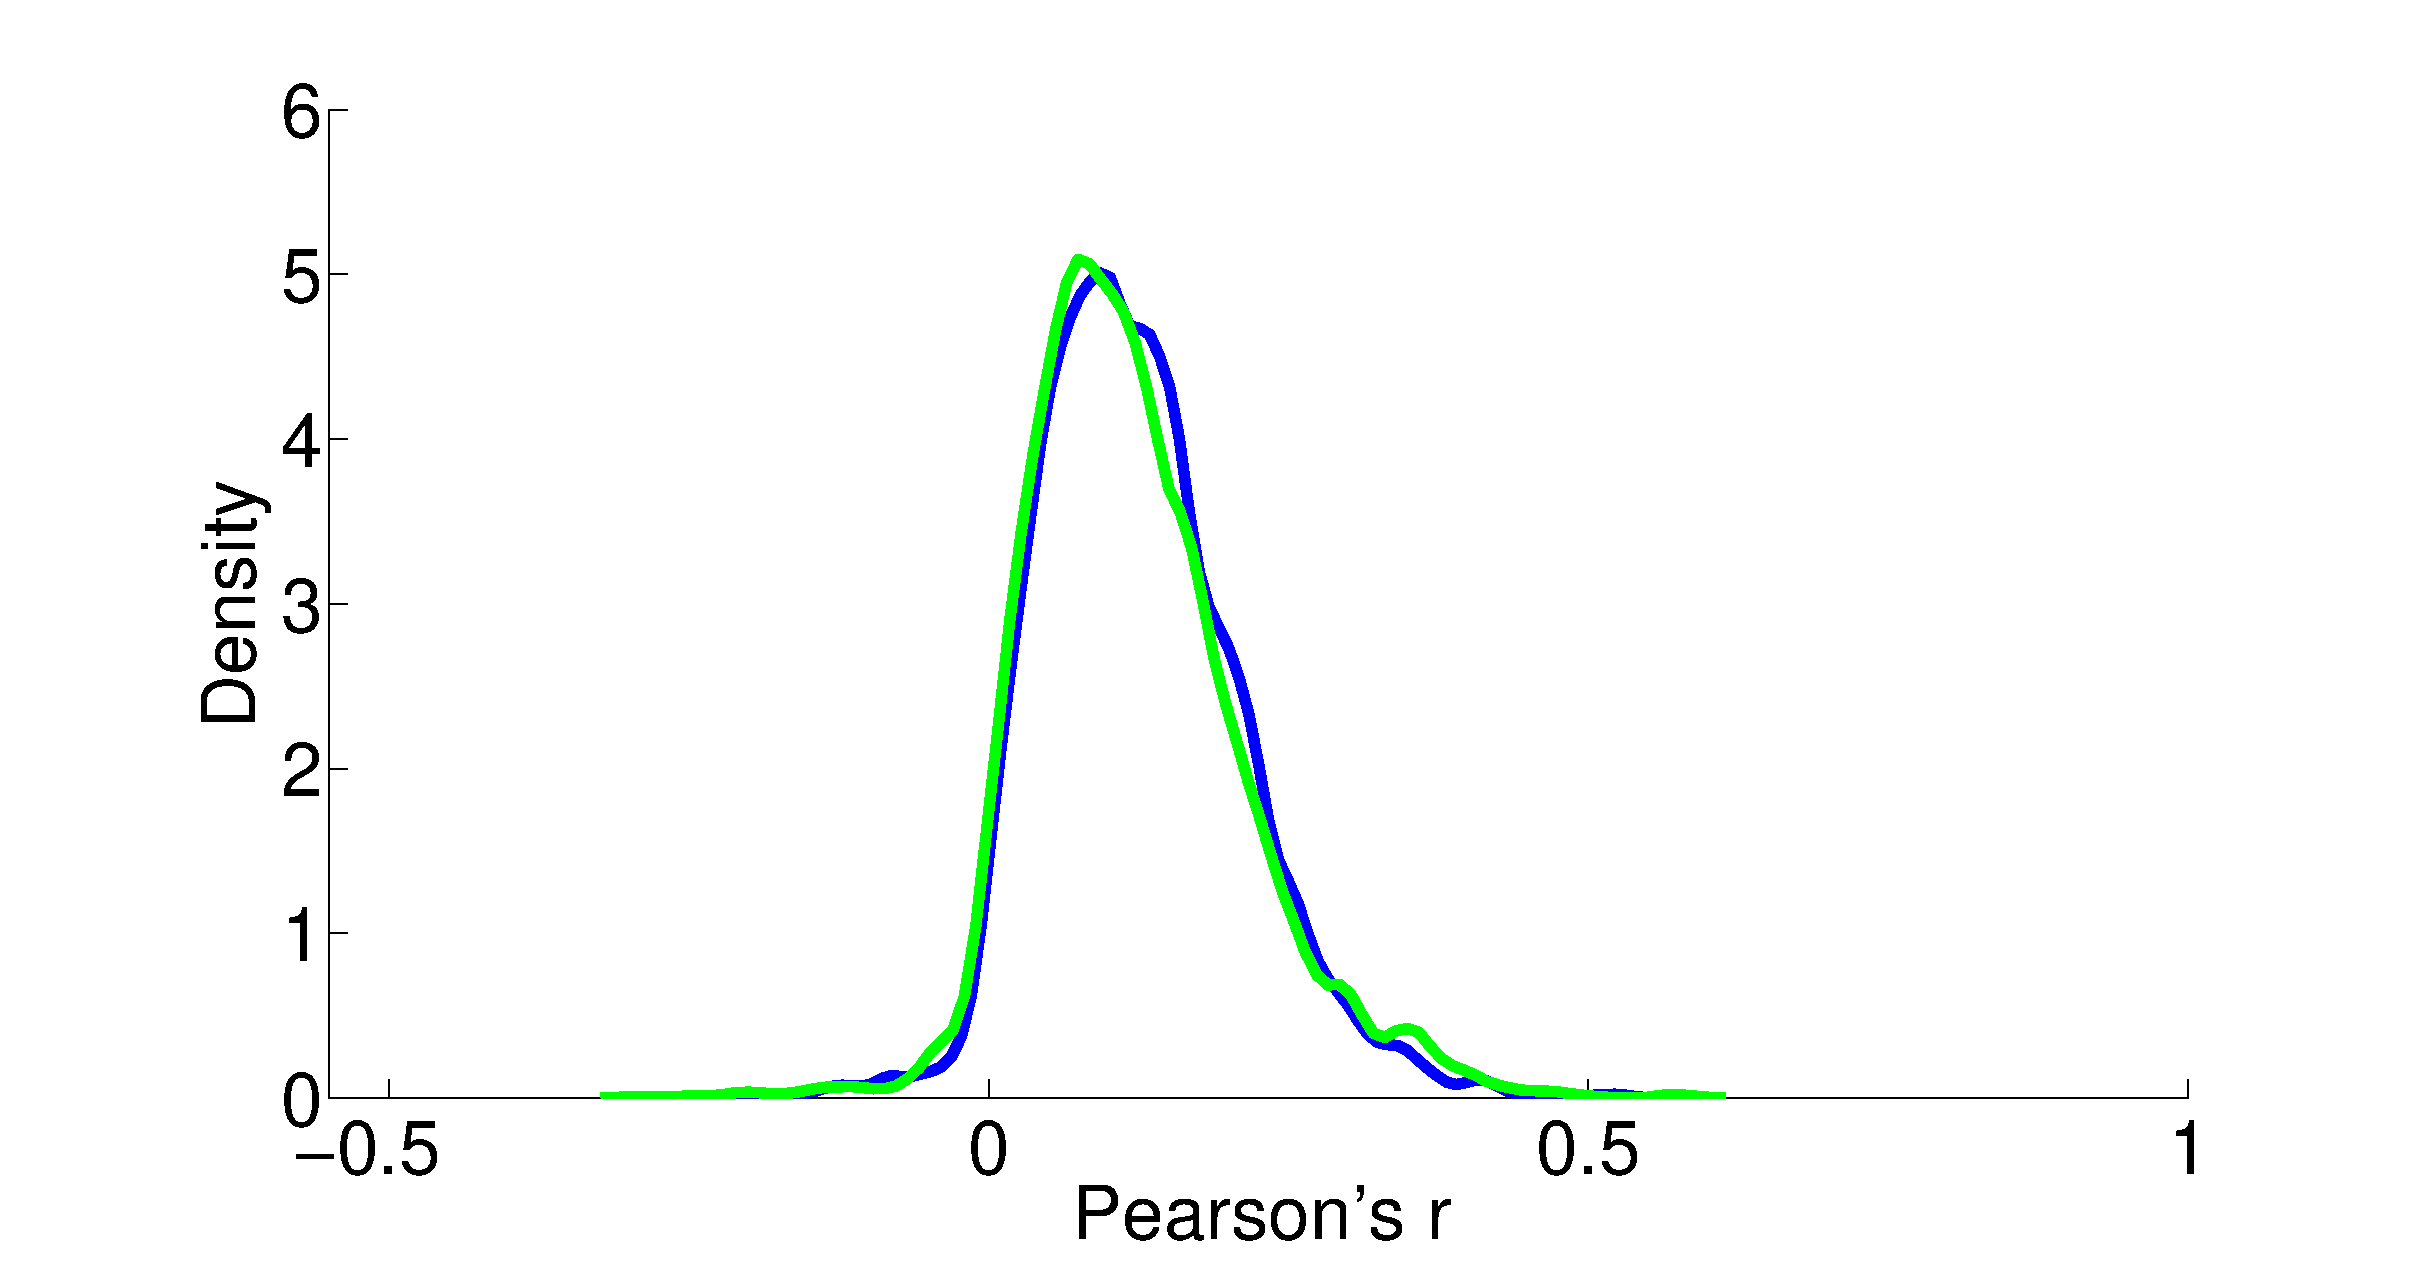
\includegraphics[width=\textwidth]{pFluxVec_dirr}
  \caption{minimally constrained} \label{fig:YpermCorrSup:B}
  \end{subfigure} 
\\
  \begin{subfigure}[b]{0.5\textwidth}
  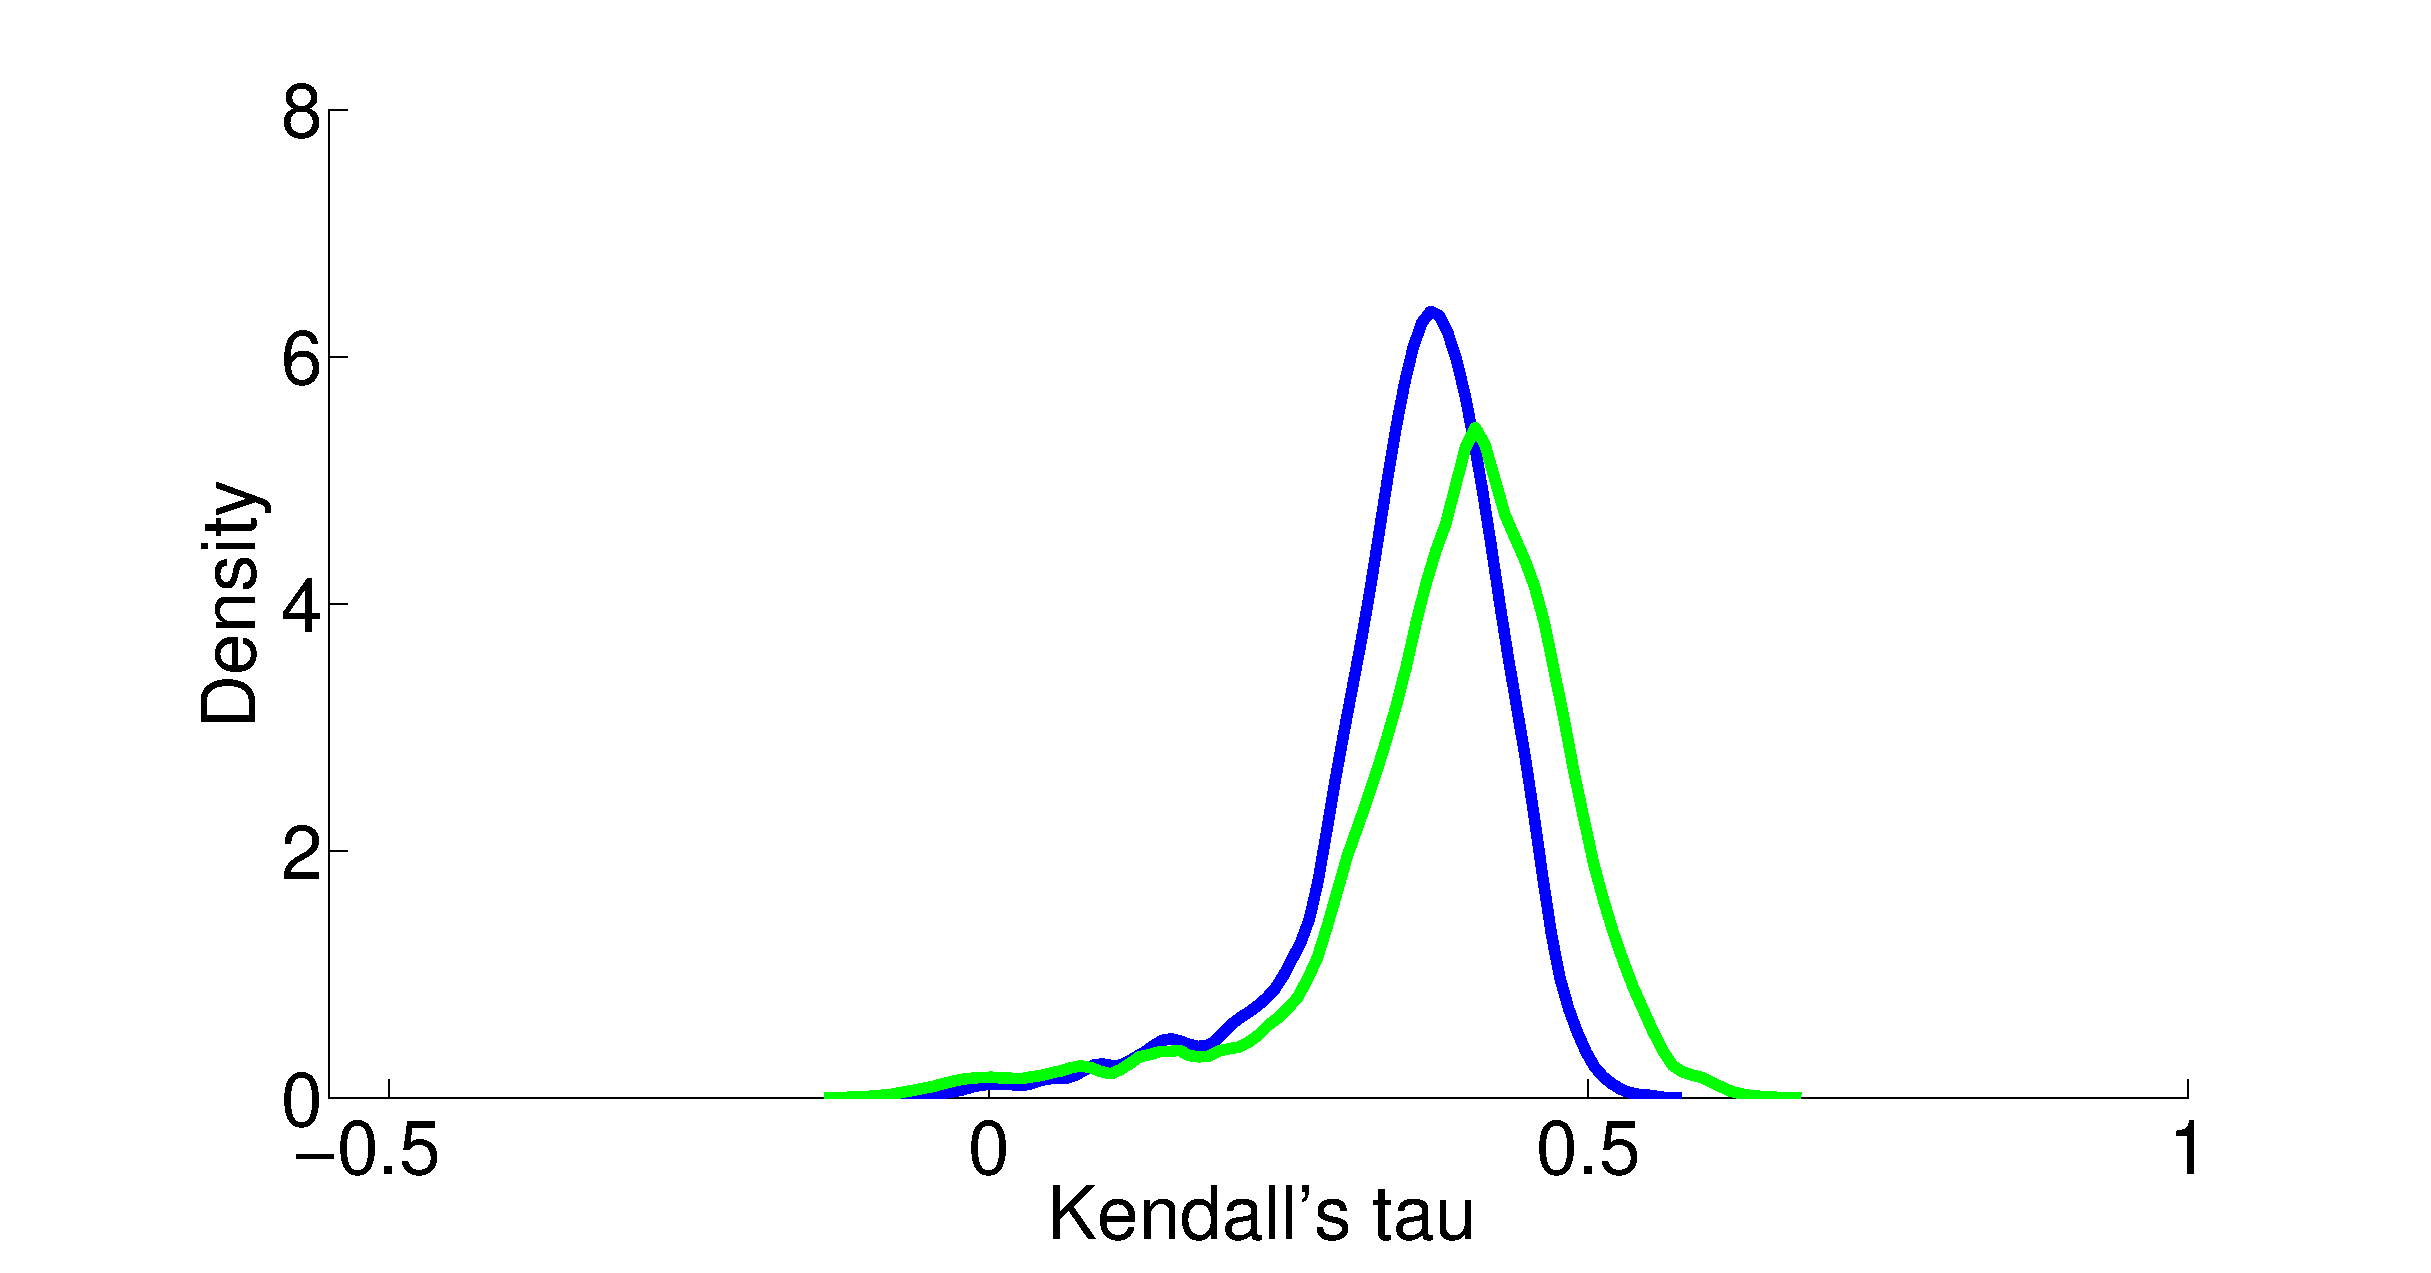
\includegraphics[width=\textwidth]{kFluxVec}
  \caption{highly constrained} \label{fig:YpermCorrSup:C}
  \end{subfigure}
&
  \begin{subfigure}[b]{0.5\textwidth}
  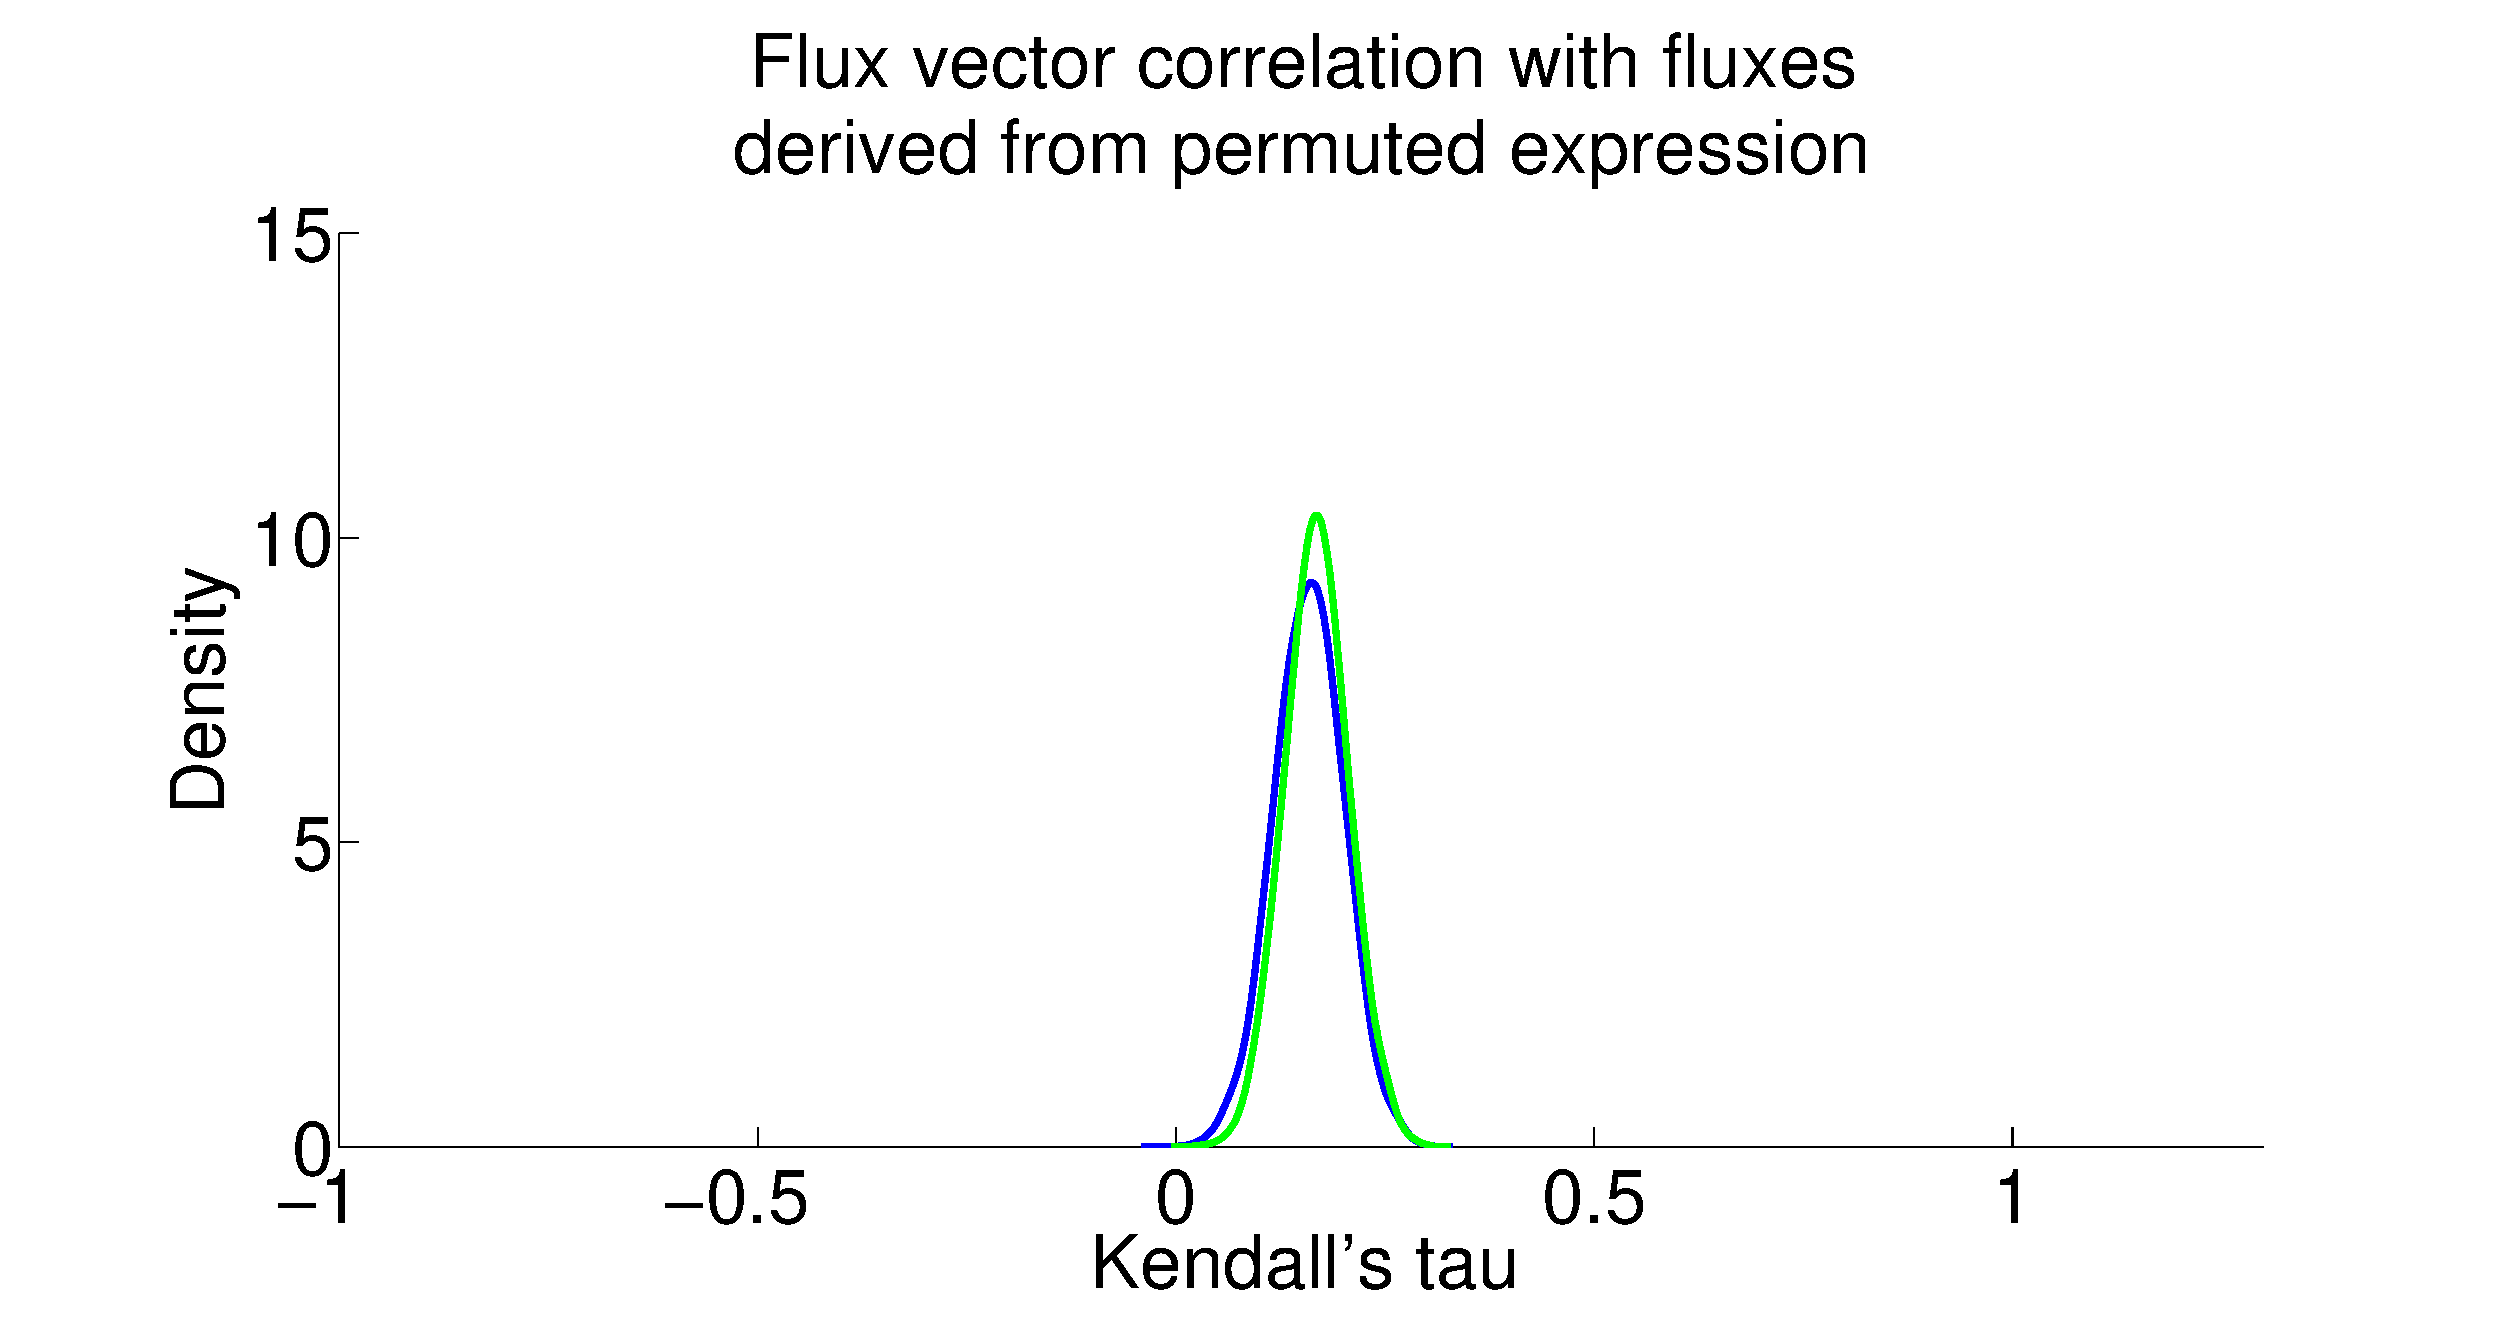
\includegraphics[width=\textwidth]{kFluxVec_dirr}
  \caption{minimally constrained} \label{fig:YpermCorrSup:D}
  \end{subfigure} 
\\
\end{tabular}
\caption{Kernel-smoothed PDFs are drawn for correlations between
the entire flux vector estimated by FALCON on permuted and unpermuted
data. Stability and correlation are effected by constraints, as there
are differences between the minimally constrained \textbf{(b, d)} and
highly constrained \textbf{(a, c)} Yeast~7 models. 5,000 permutation
replicates were performed in all cases.}
\label{fig:YpermCorrSup}
\end{figure}
\FloatBarrier

\begin{figure}[!htb]
\begin{tabular}{cc}
  \begin{subfigure}[b]{0.5\textwidth}
  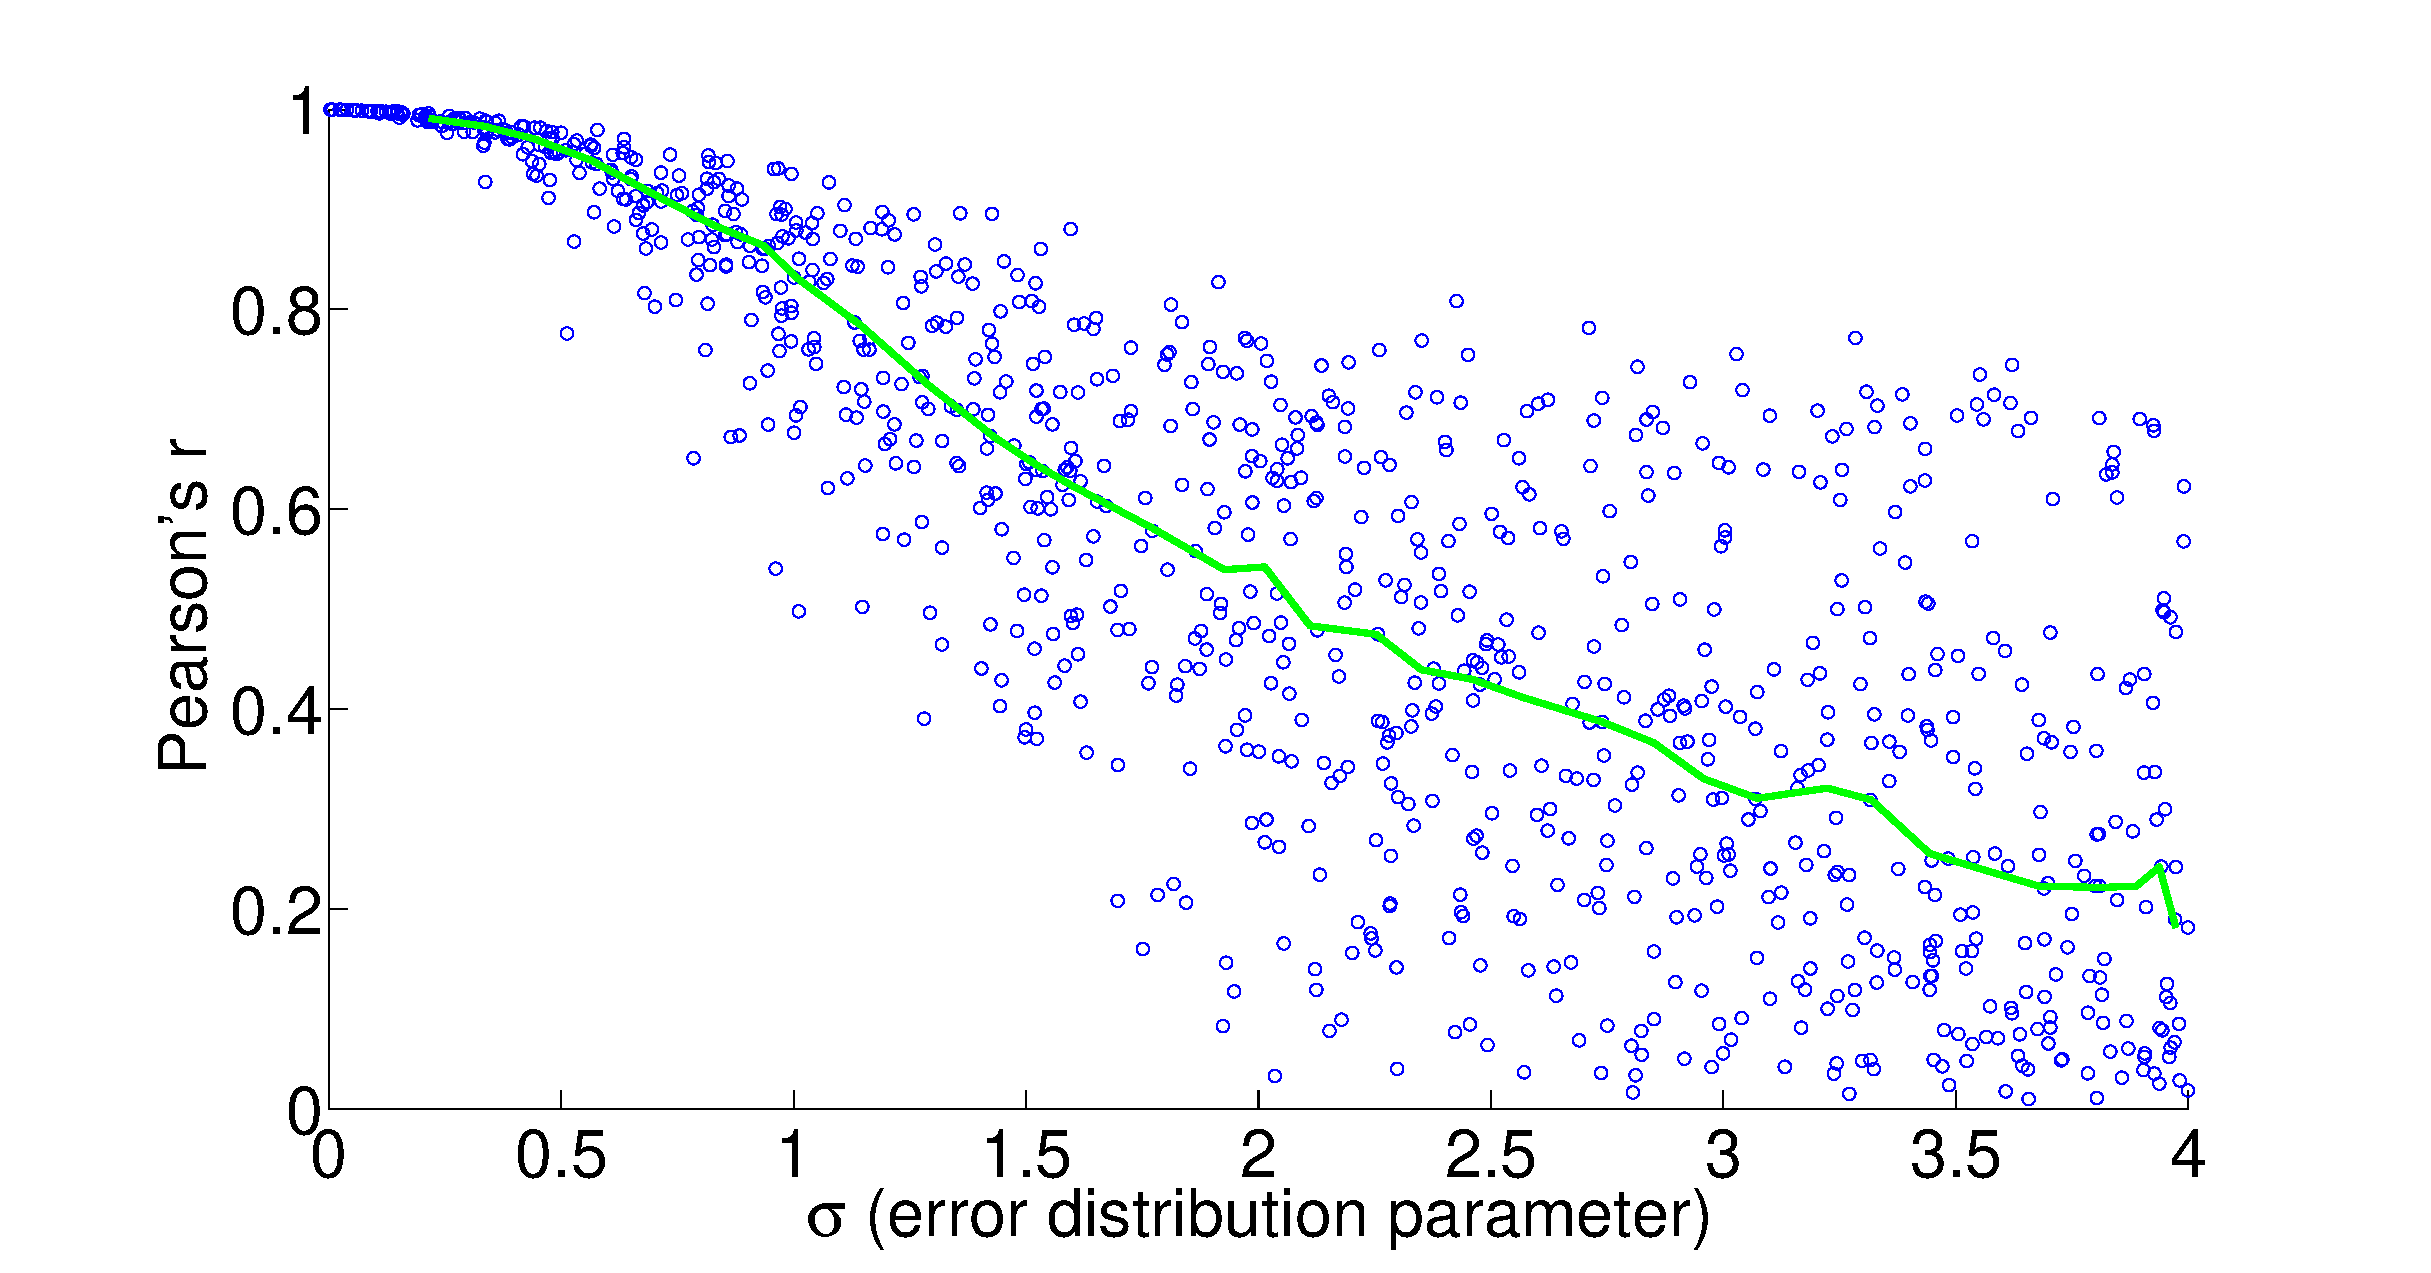
\includegraphics[width=\textwidth]{noise_rec2EC}
  \caption{} \label{fig:ExpSensRec2:A}
  \end{subfigure}
&
  \begin{subfigure}[b]{0.5\textwidth}
  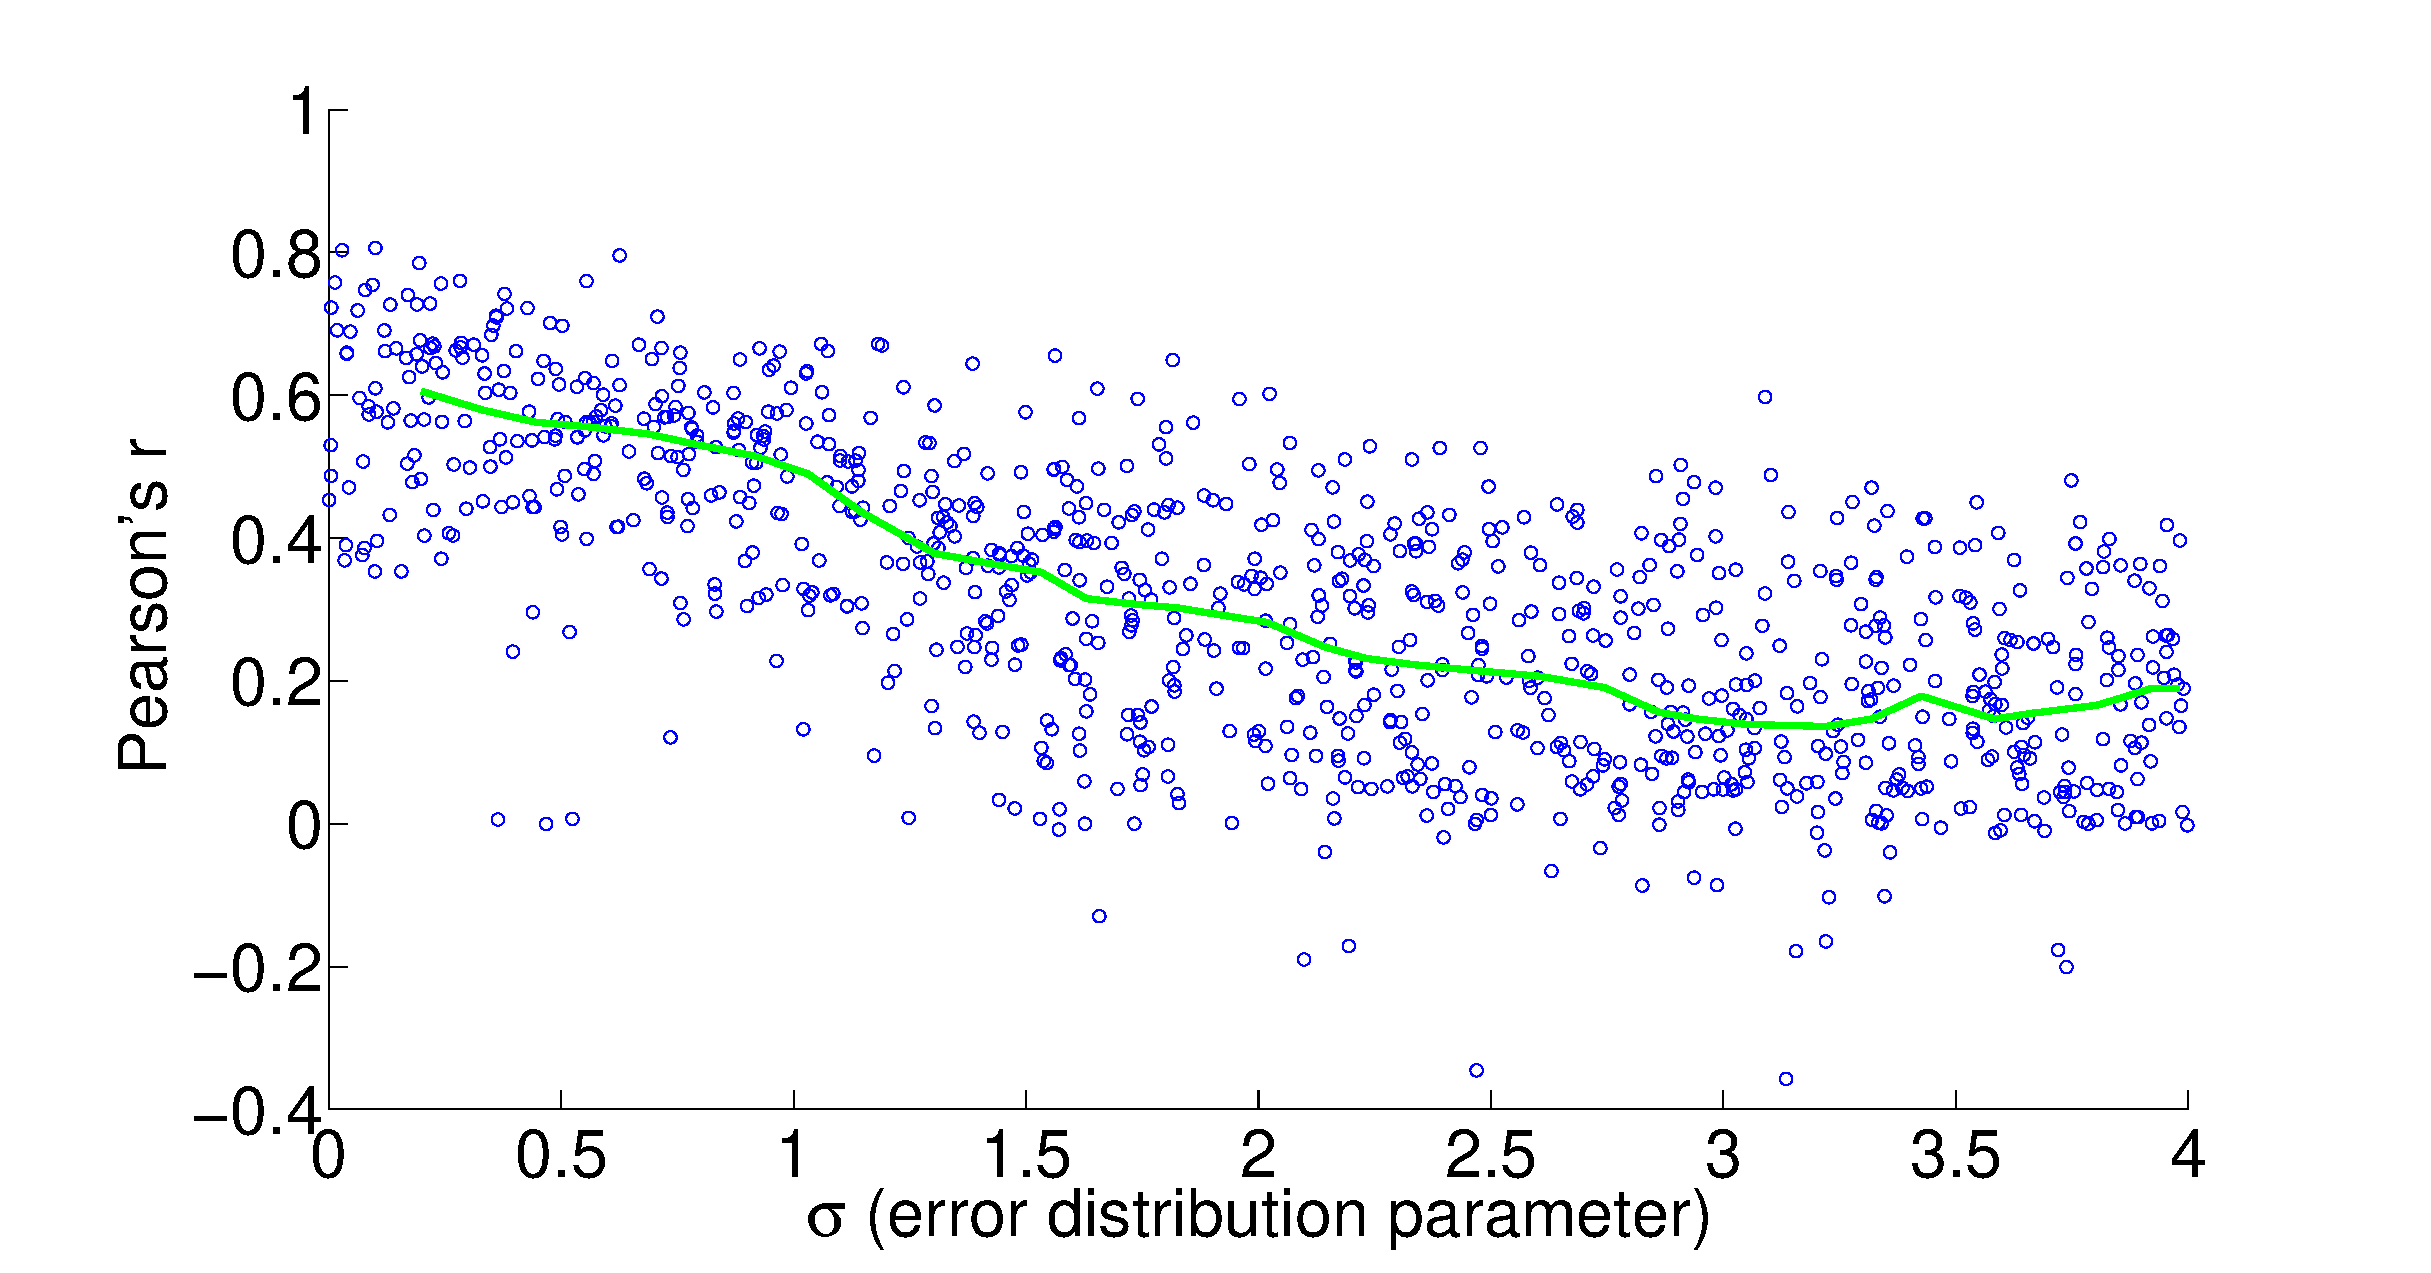
\includegraphics[width=\textwidth]{noise_rec2rpmiCORE_all_flux}
  \caption{} \label{fig:ExpSensRec2:B}
  \end{subfigure} 
\\
  \begin{subfigure}[b]{0.5\textwidth}
  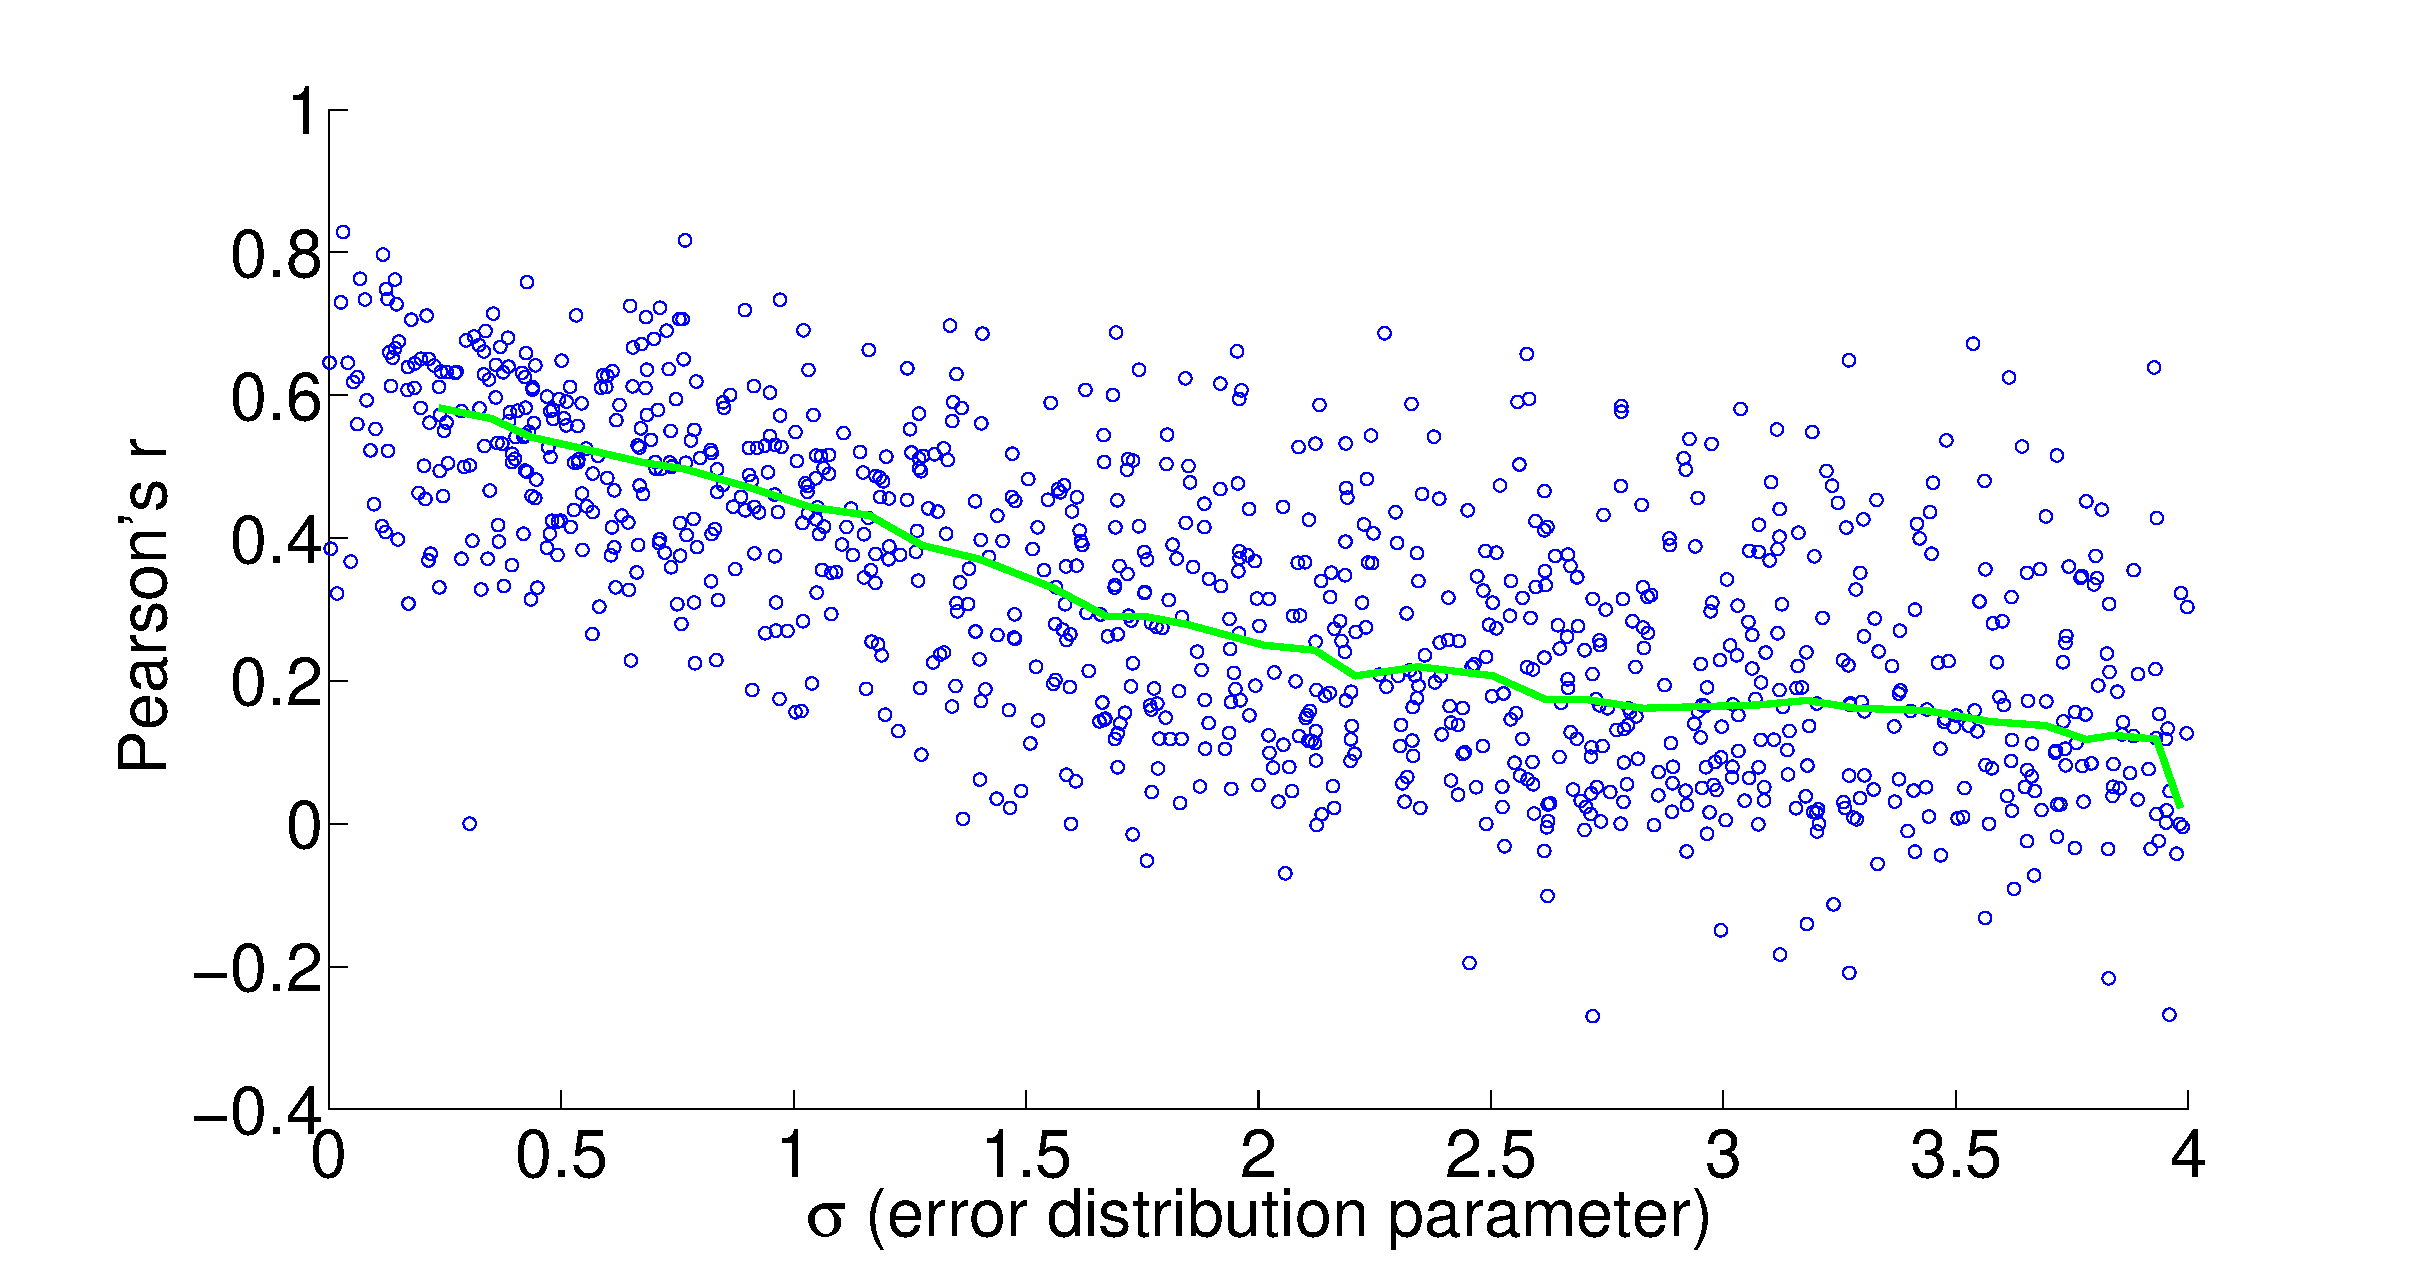
\includegraphics[width=\textwidth]{noise_rec2rpmiCORE_ec_flux}
  \caption{} \label{fig:ExpSensRec2:C}
  \end{subfigure} 
&
  \begin{subfigure}[b]{0.5\textwidth}
  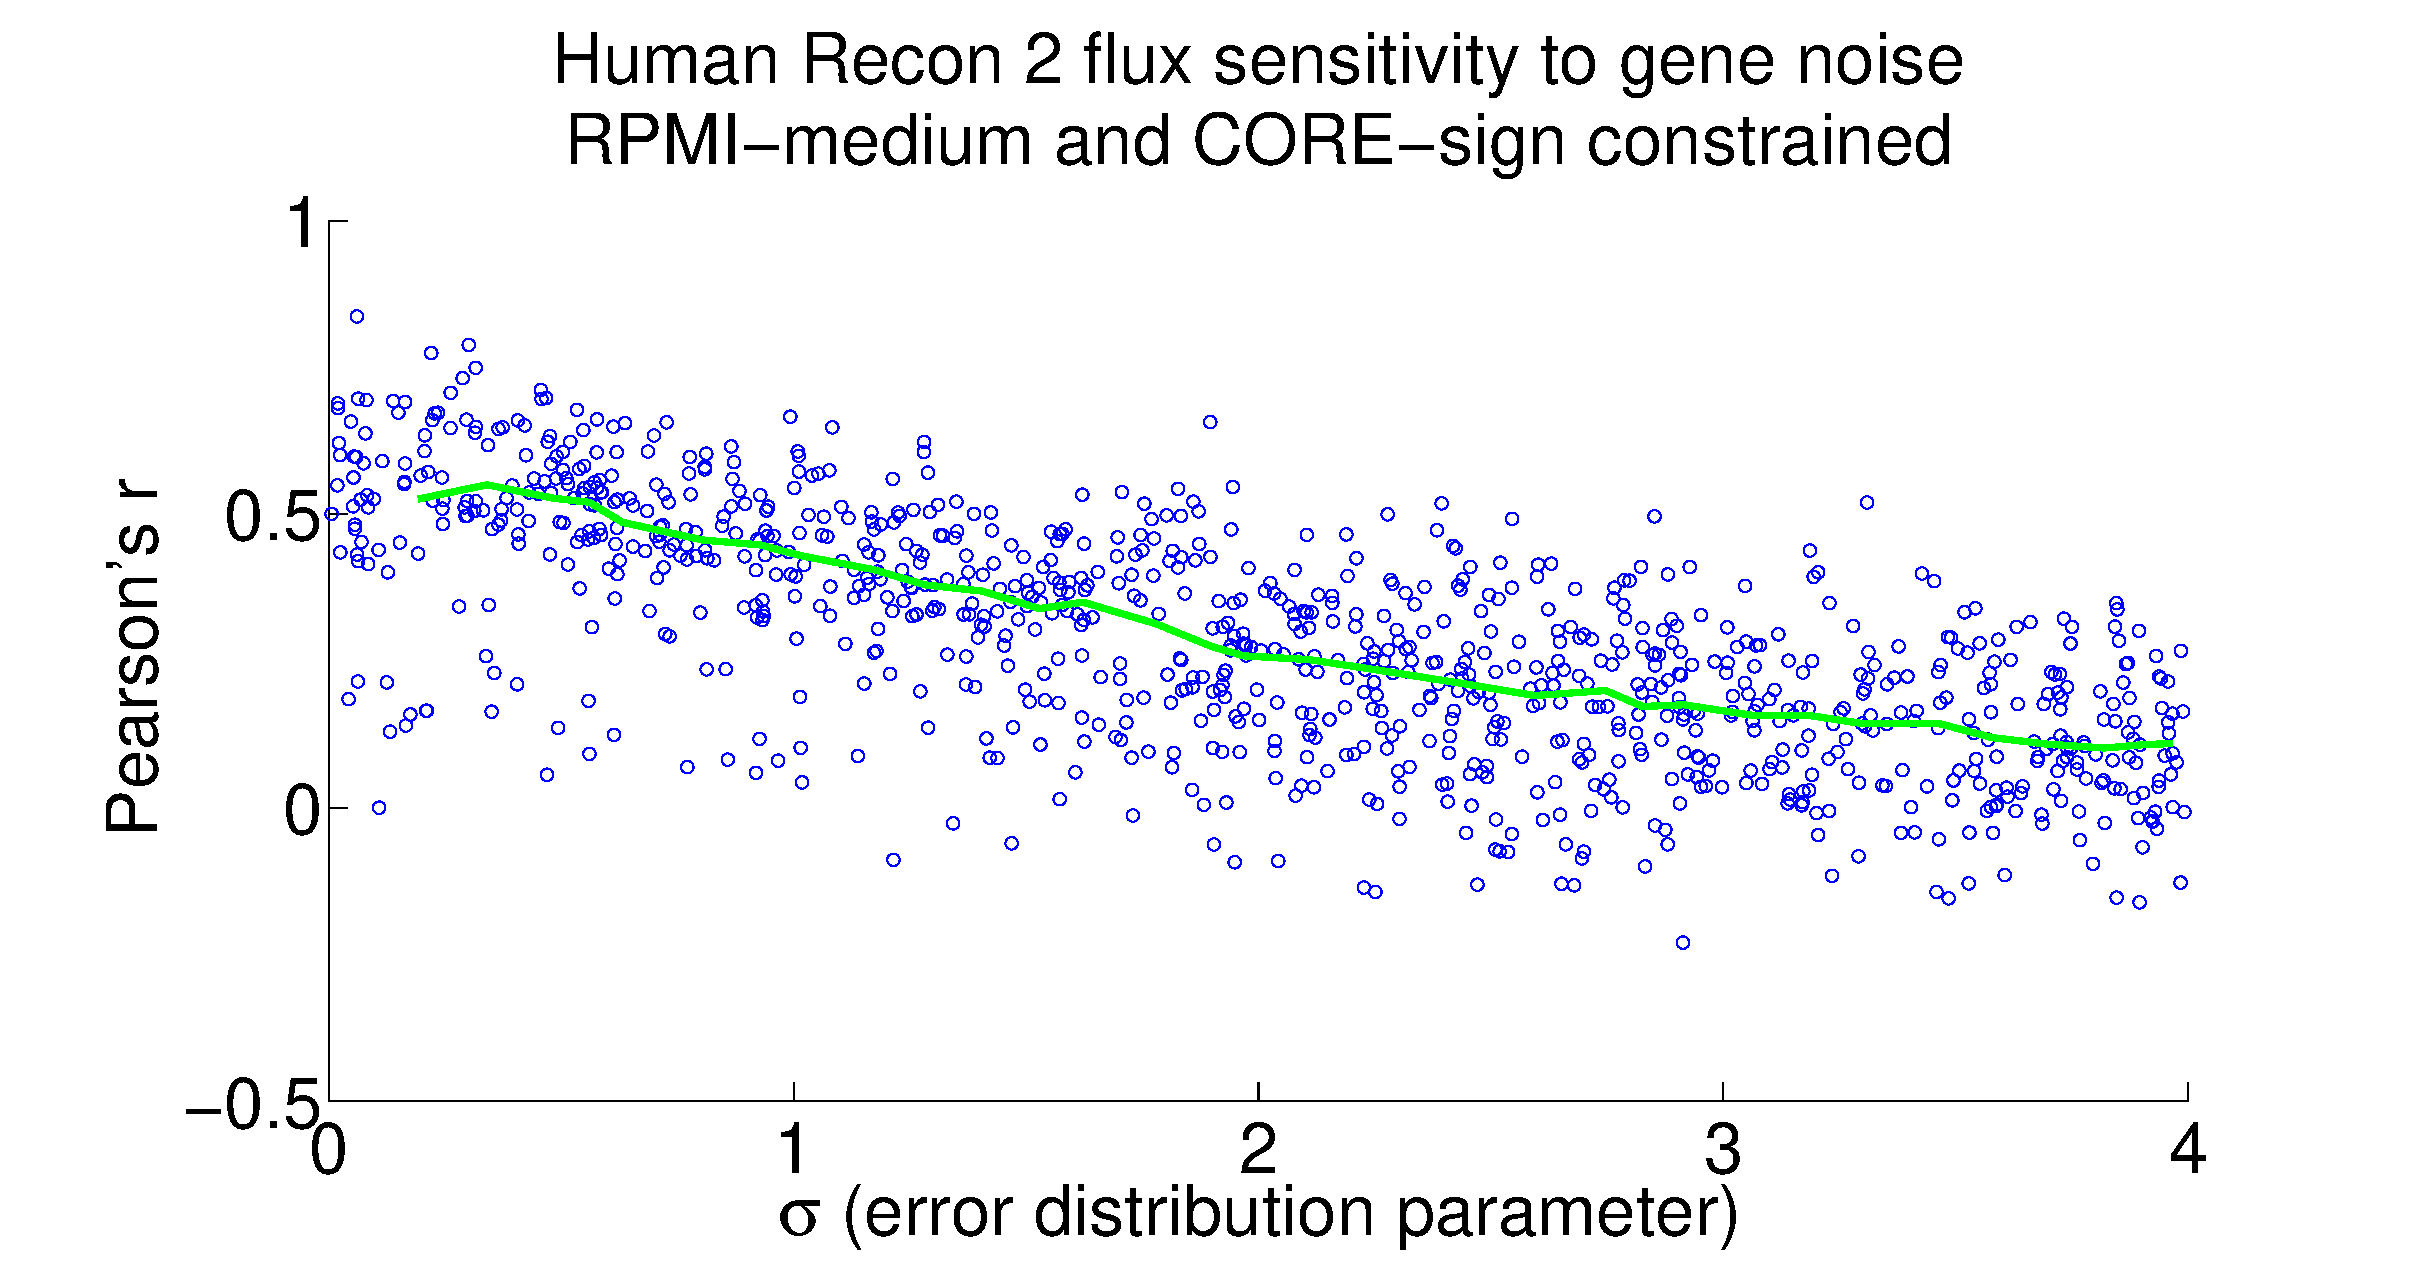
\includegraphics[width=\textwidth]{noise_rec2rpmiCORE_flux}
  \caption{} \label{fig:ExpSensRec2:D}
  \end{subfigure} 
\\
  \begin{subfigure}[b]{0.5\textwidth}
  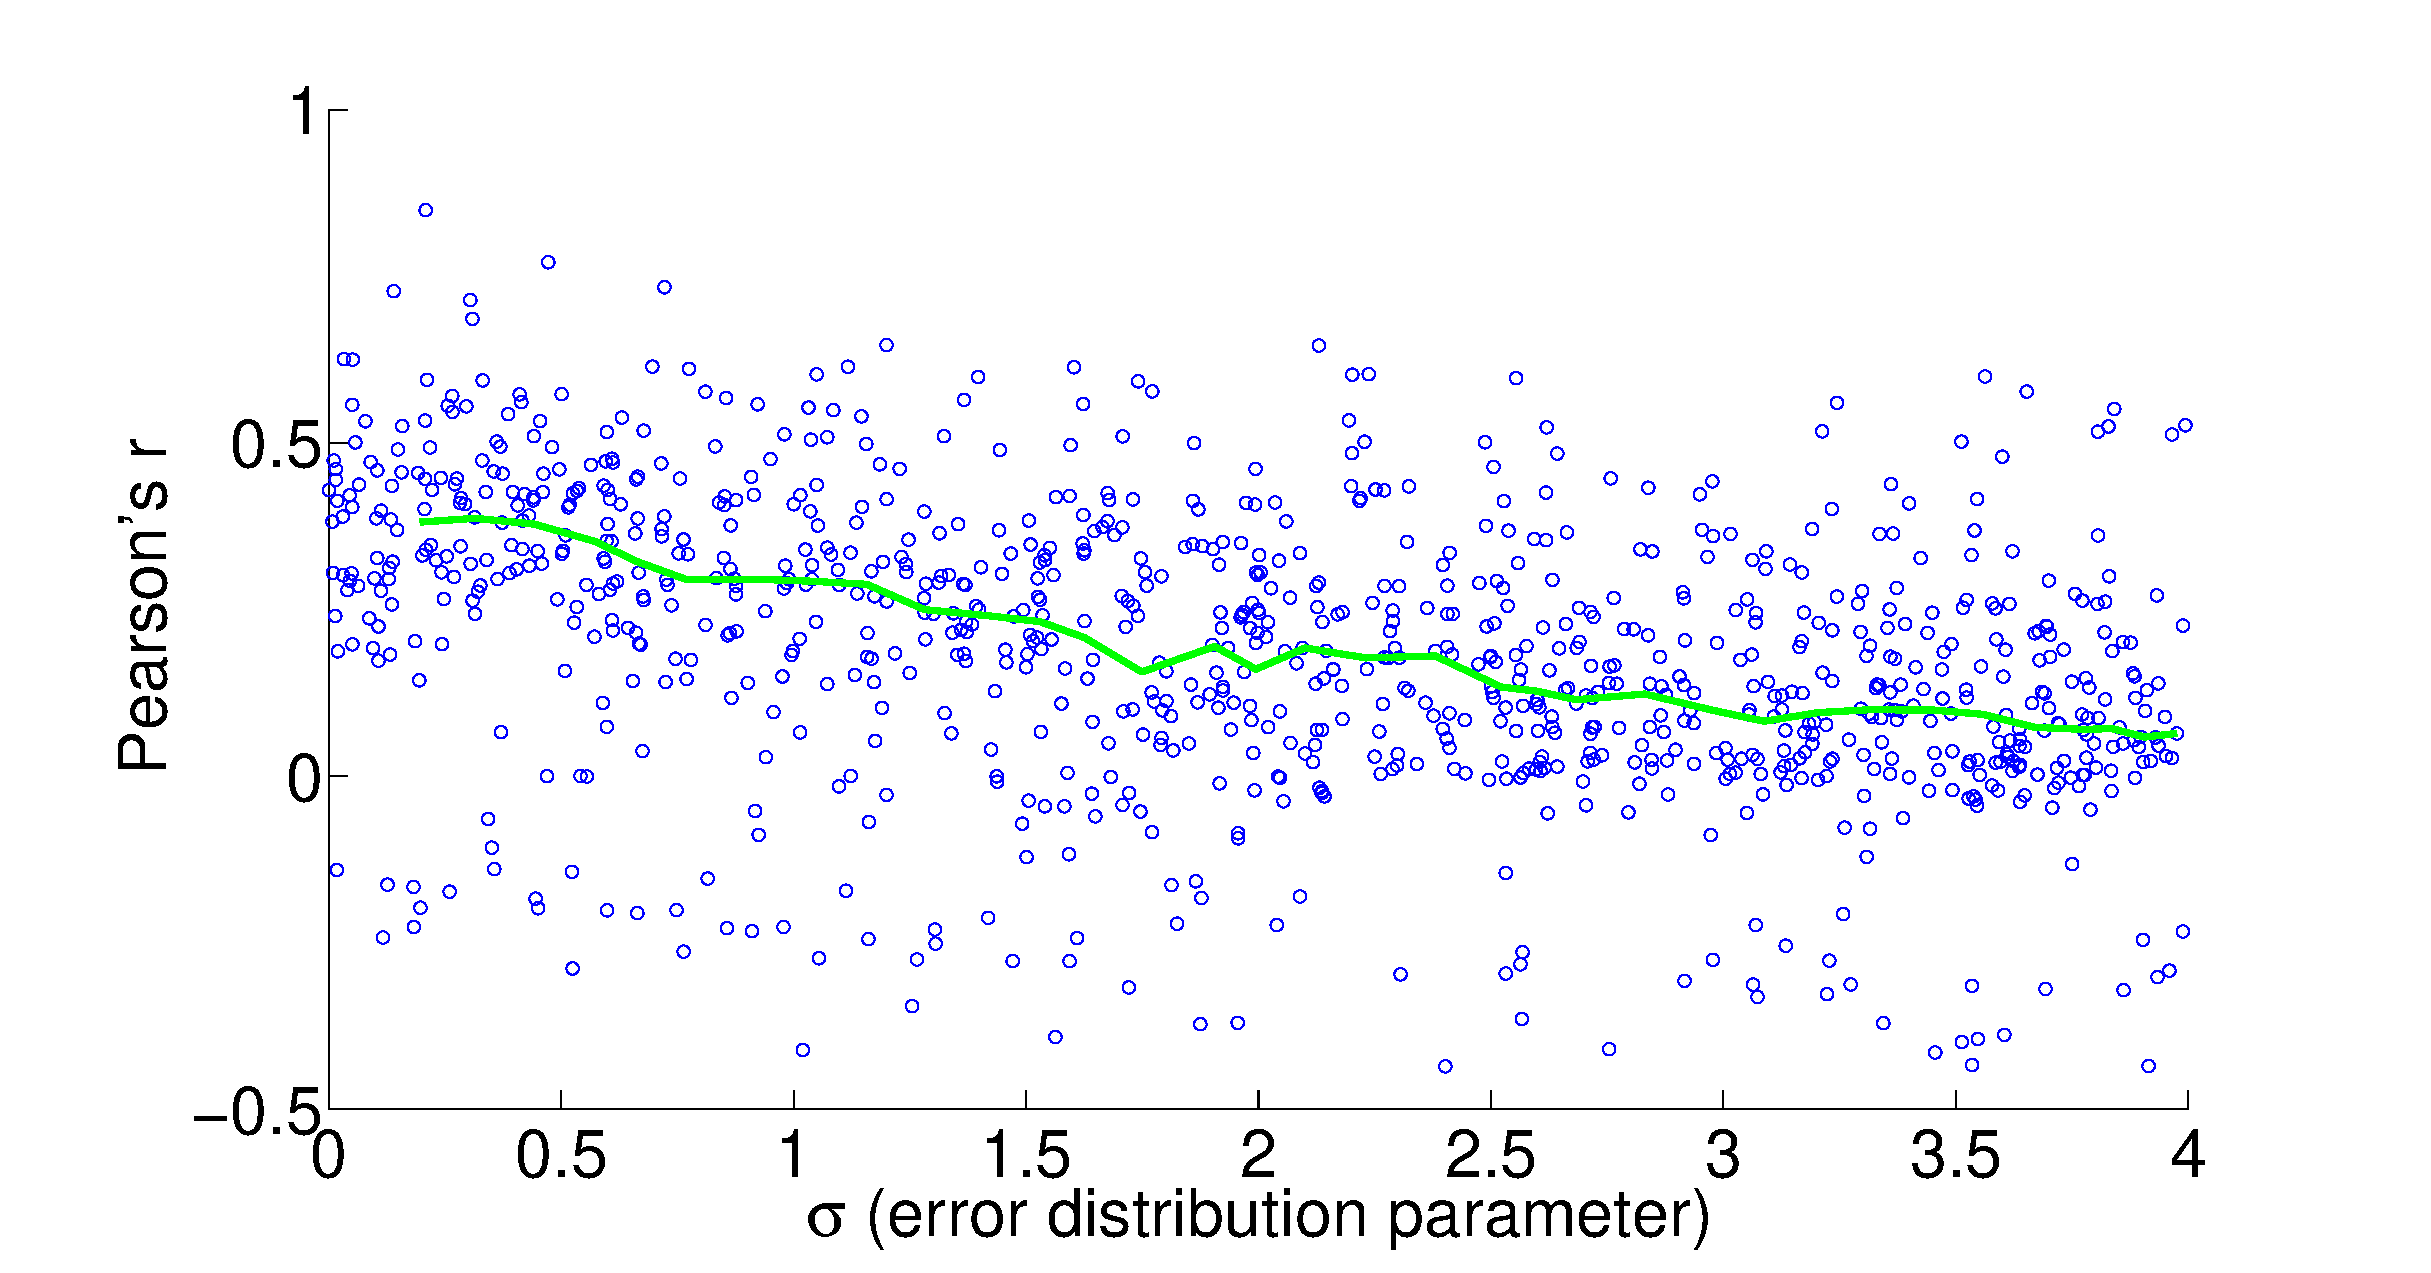
\includegraphics[width=\textwidth]{noise_rec2rpmi_flux}
  \caption{} \label{fig:ExpSensRec2:E}
  \end{subfigure} 
&
  \begin{subfigure}[b]{0.5\textwidth}
  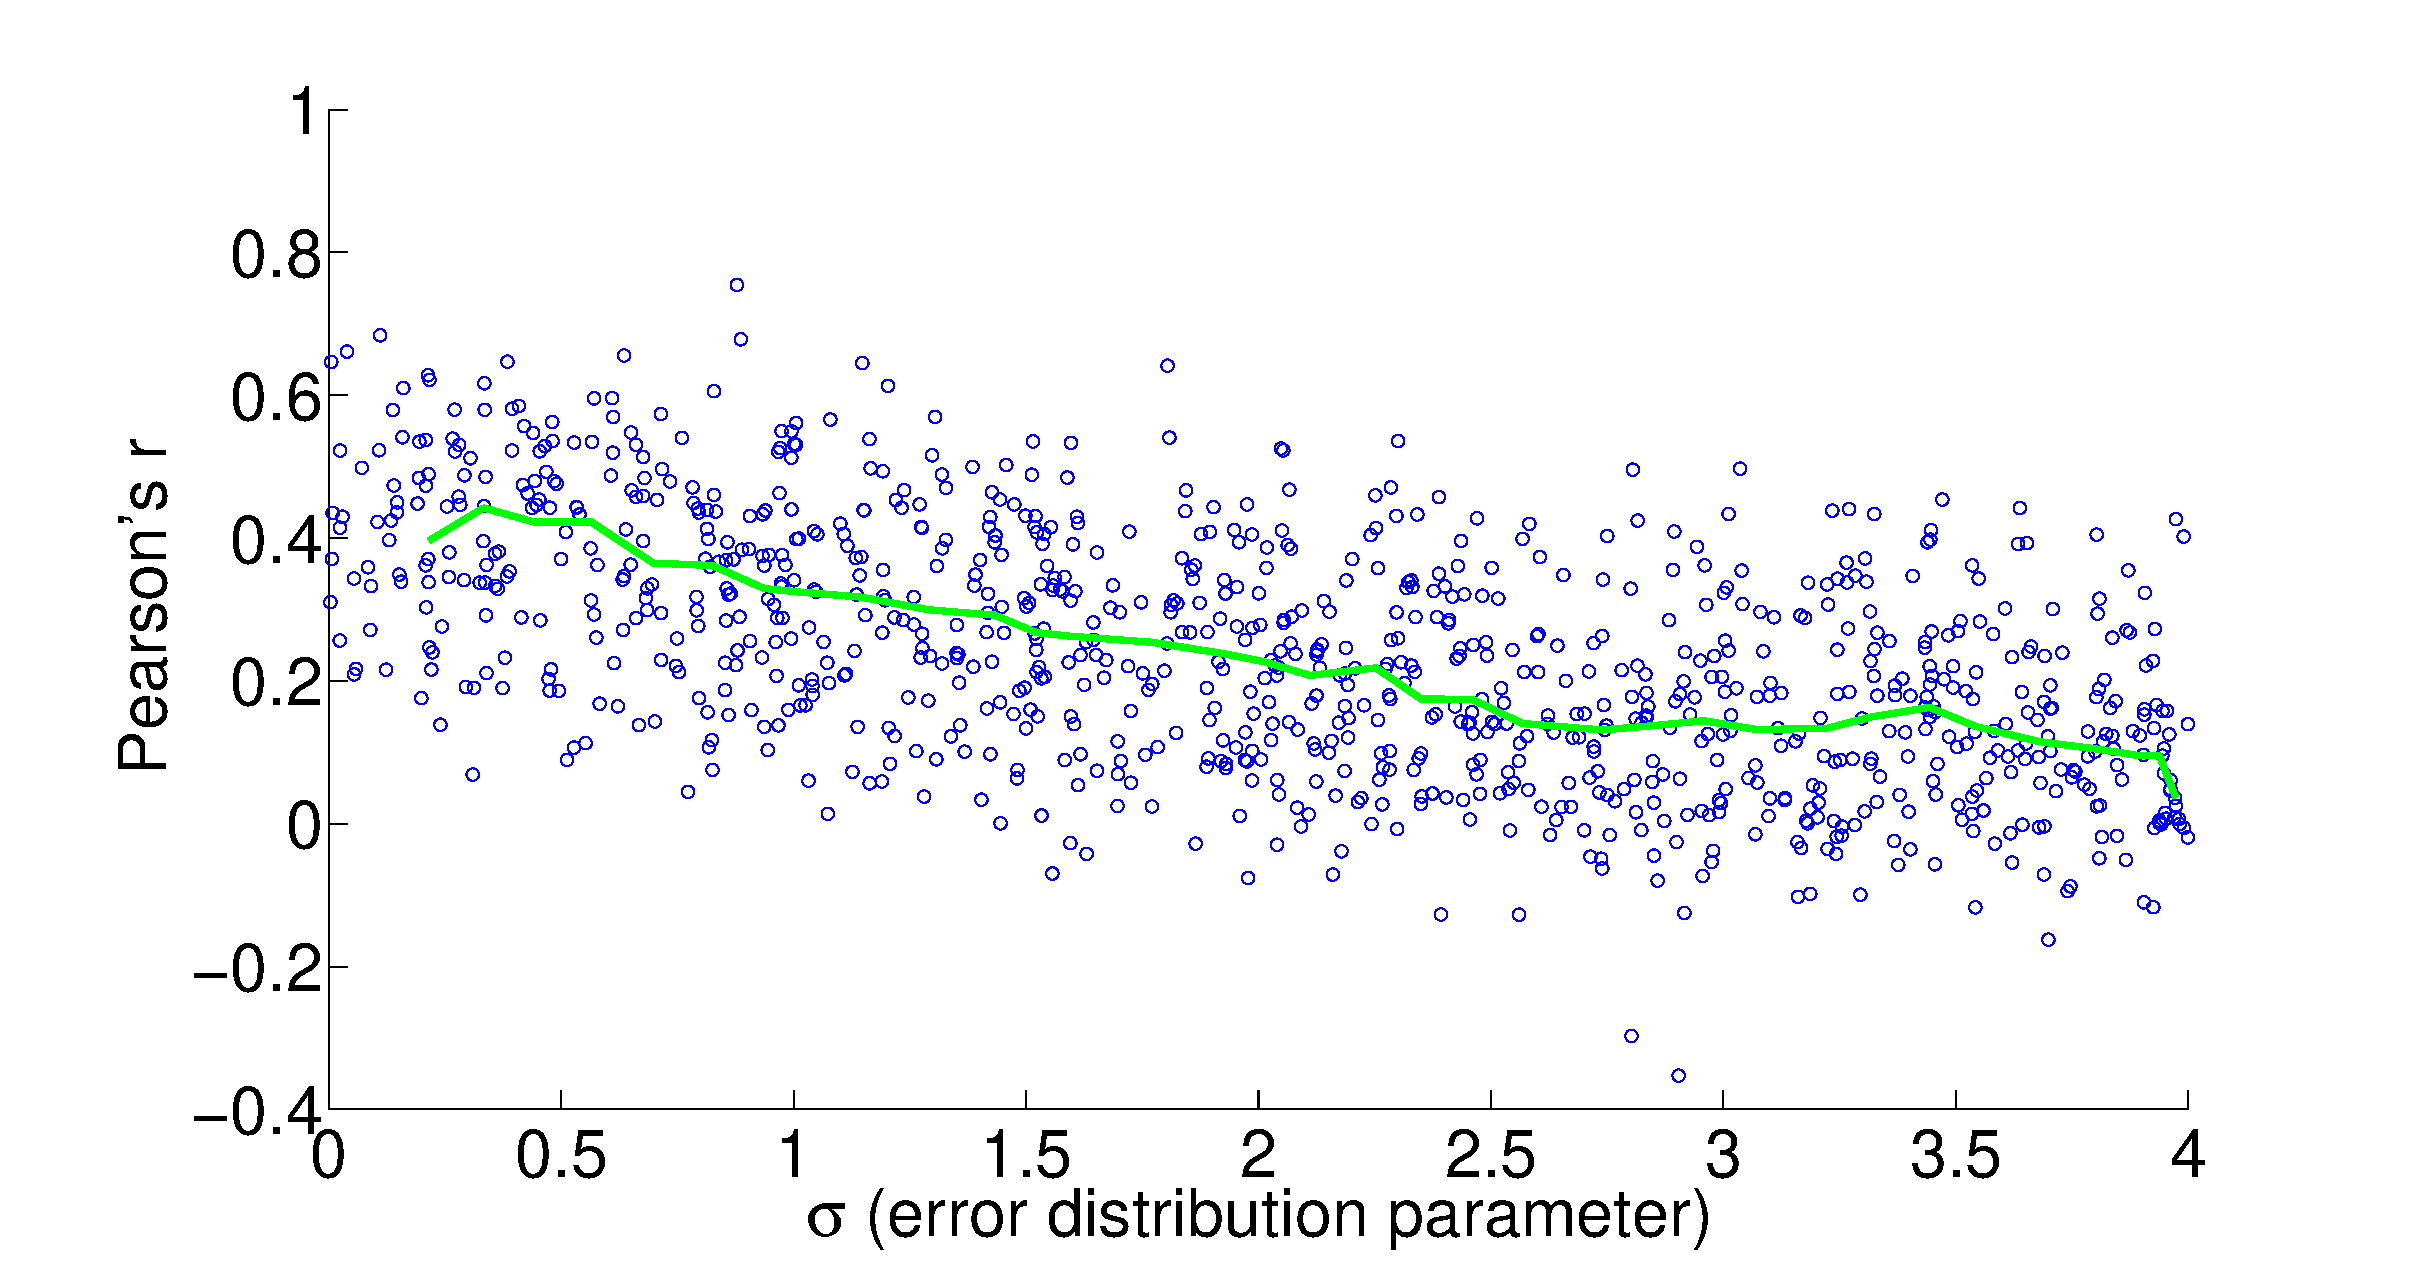
\includegraphics[width=\textwidth]{noise_rec2flux}
  \caption{} \label{fig:ExpSensRec2:F}
  \end{subfigure} 
\\
\end{tabular}
\caption{ These figures are generated in the same way as those in
\Fig~\ref{fig:ExpSens}, but for Human Recon~2 instead of Yeast~7. We
used several different constraint sets based on experimental media and
exometabolic flux data in the NCI-60 cell lines \protect\citep{Jain2012}. 
These constraints were applied cumulatively, and are
listed in the order of most constrained \textbf{(b)} to least
constrained \textbf{(f)}. Included are default Recon~2 constraints
\textbf{(f)}, RPMI media constraints (\textbf{e}; function
\texttt{constrainCoReMinMaxSign}; 556 constraints), exometabolic
fluxes with a common sign across all cell lines and replicates
(\textbf{d}; function \texttt{constrainCoReMinMaxSign}; 567 cumulative
constraints), enzymatic reaction directionality constraints from a
linear MoMA fitting on the exometabolic flux data that agree across
all NCI-60 cell lines (\textbf{c};
\texttt{constrainImputed\-Internal}; 593 cumulative constraints), and
the same again considering all reactions instead of only enzymatic
reactions (\textbf{b}; 618 cumulative constraints).}
\label{fig:ExpSensRec2}
\end{figure}
\FloatBarrier


%\setlength\fboxsep{0pt}
%\setlength\fboxrule{0.5pt}

\begin{figure}[!htb]
\begin{tabular}{cc}
  \begin{subfigure}[b]{0.5\textwidth}   % l   b   r   t
  %\fbox{
  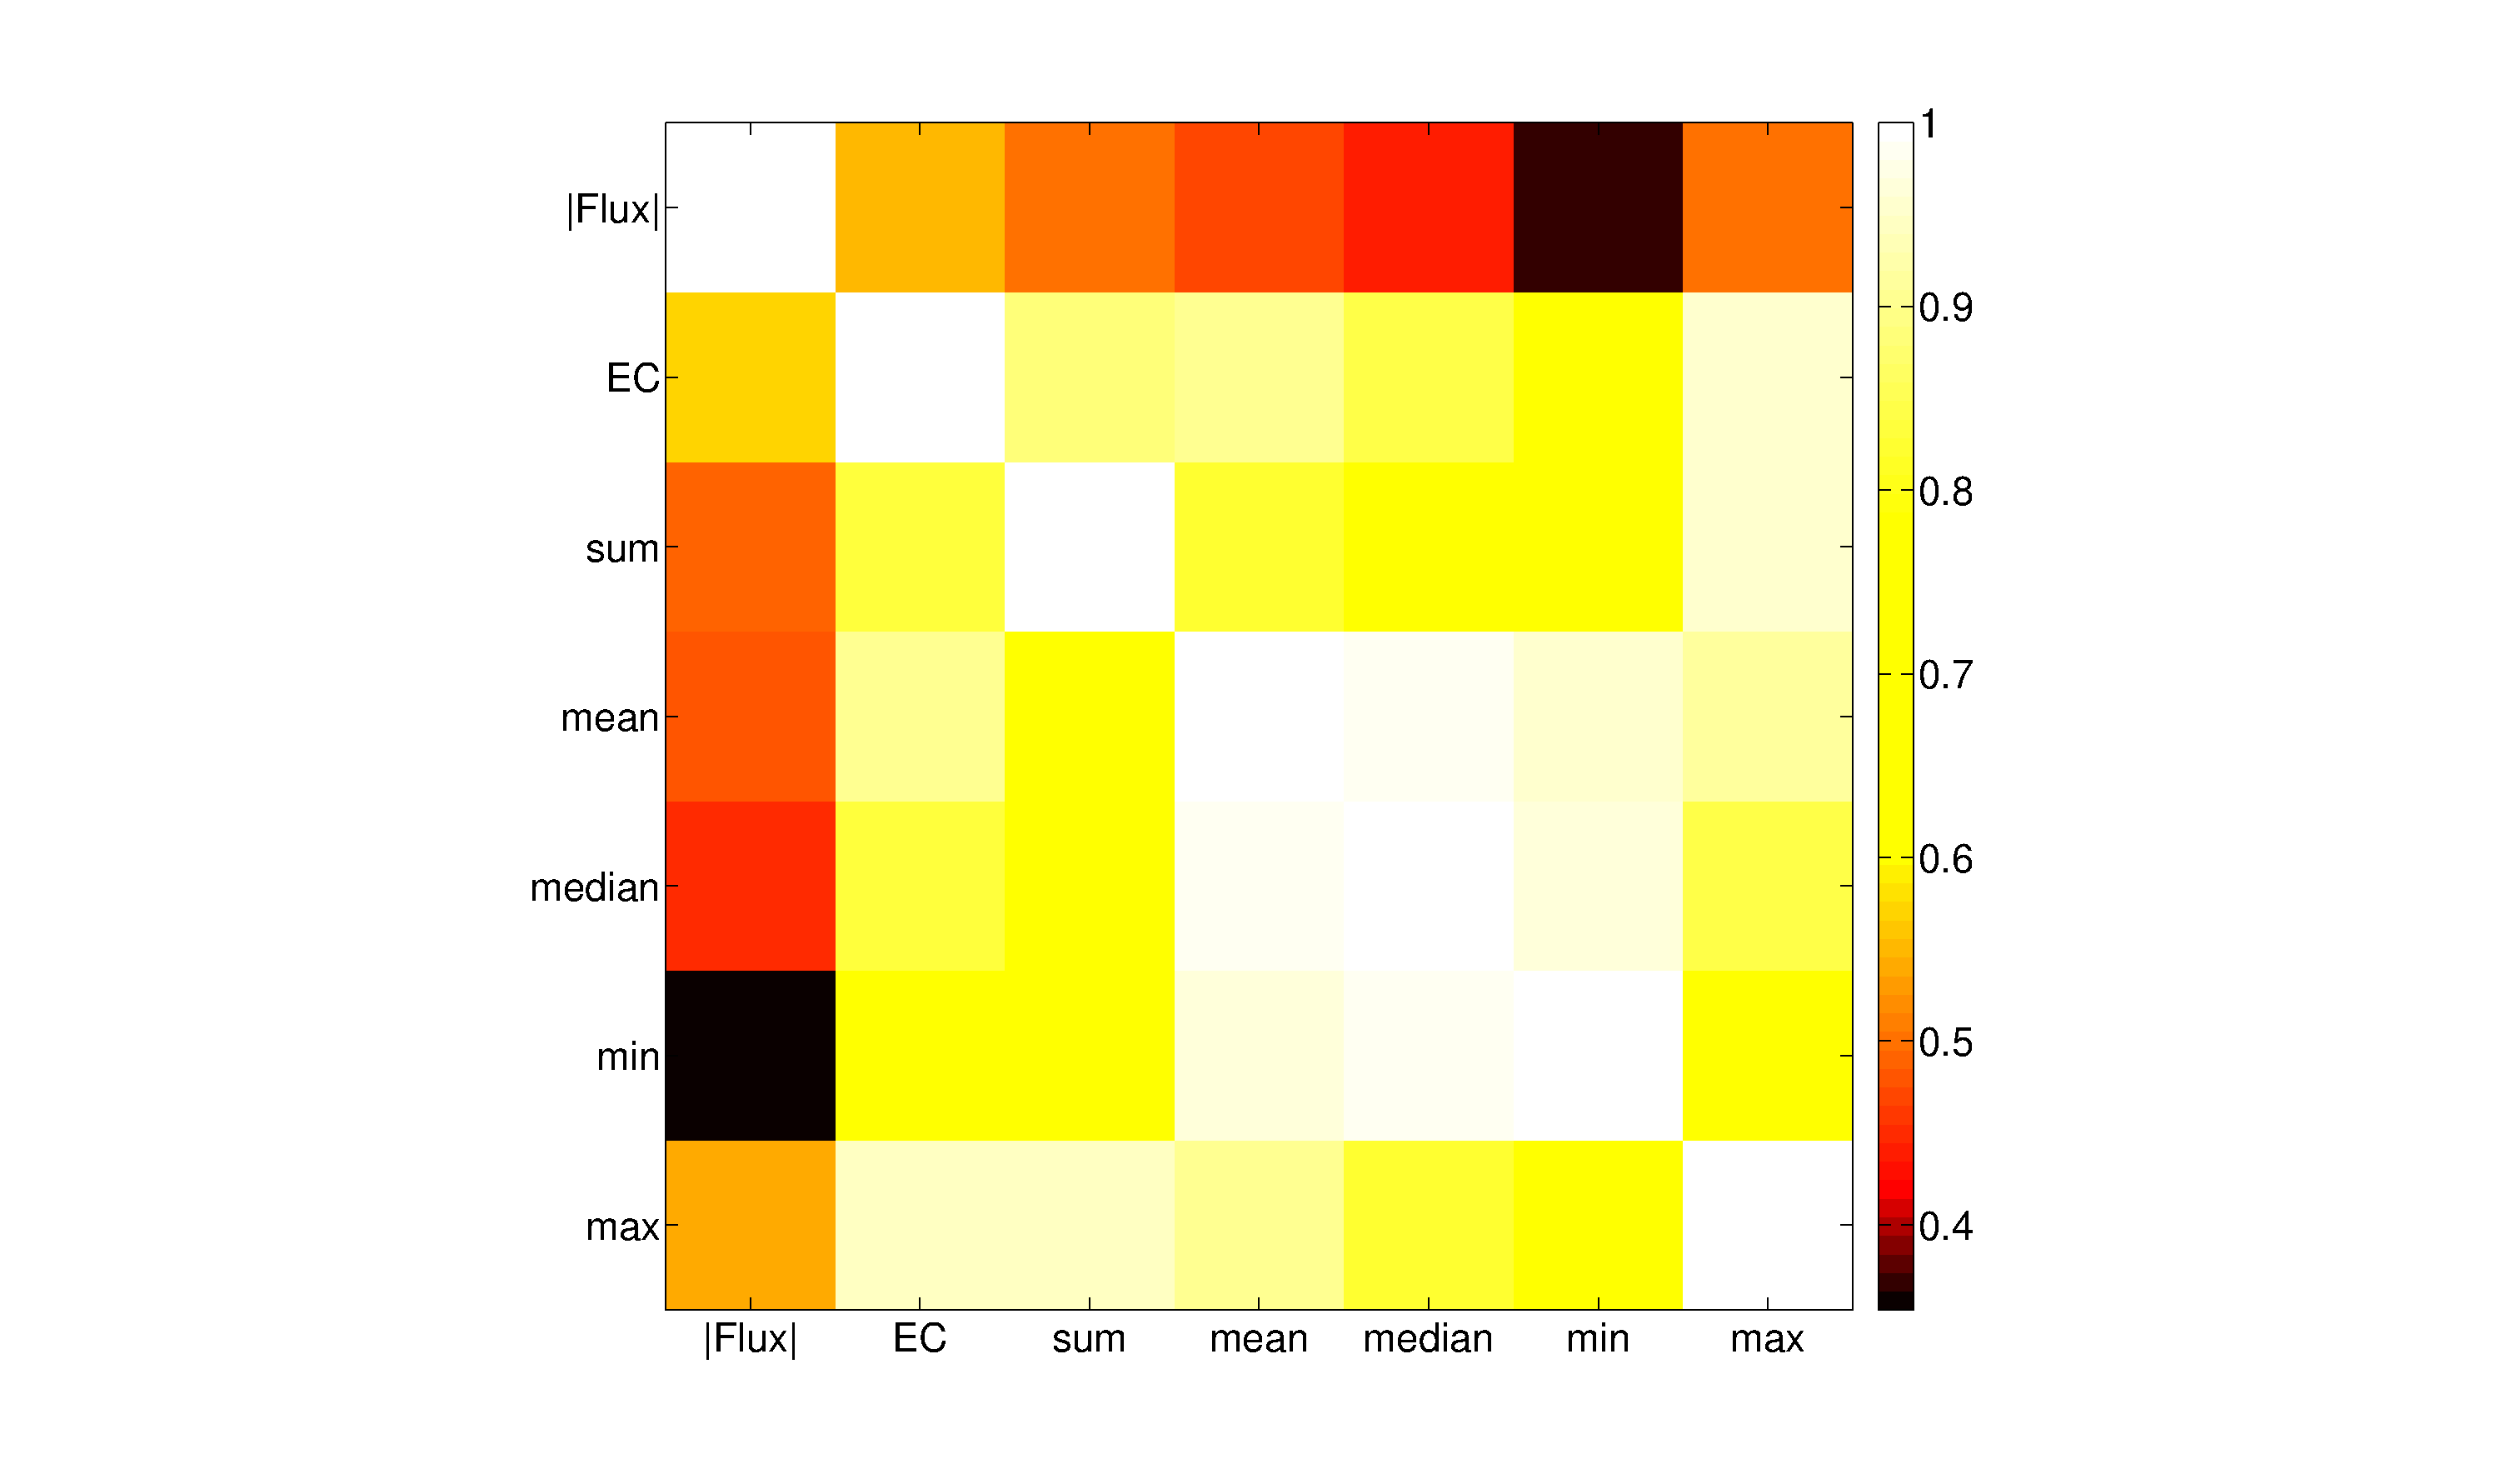
\includegraphics[width=\textwidth, trim=9cm 1.2cm 9cm 1cm, clip=true]
    {YeastExpFluxCompare}
  %}
  \caption{yeast} \label{fig:FluxExpCmp:A}
  \end{subfigure}
&
  \begin{subfigure}[b]{0.5\textwidth}
  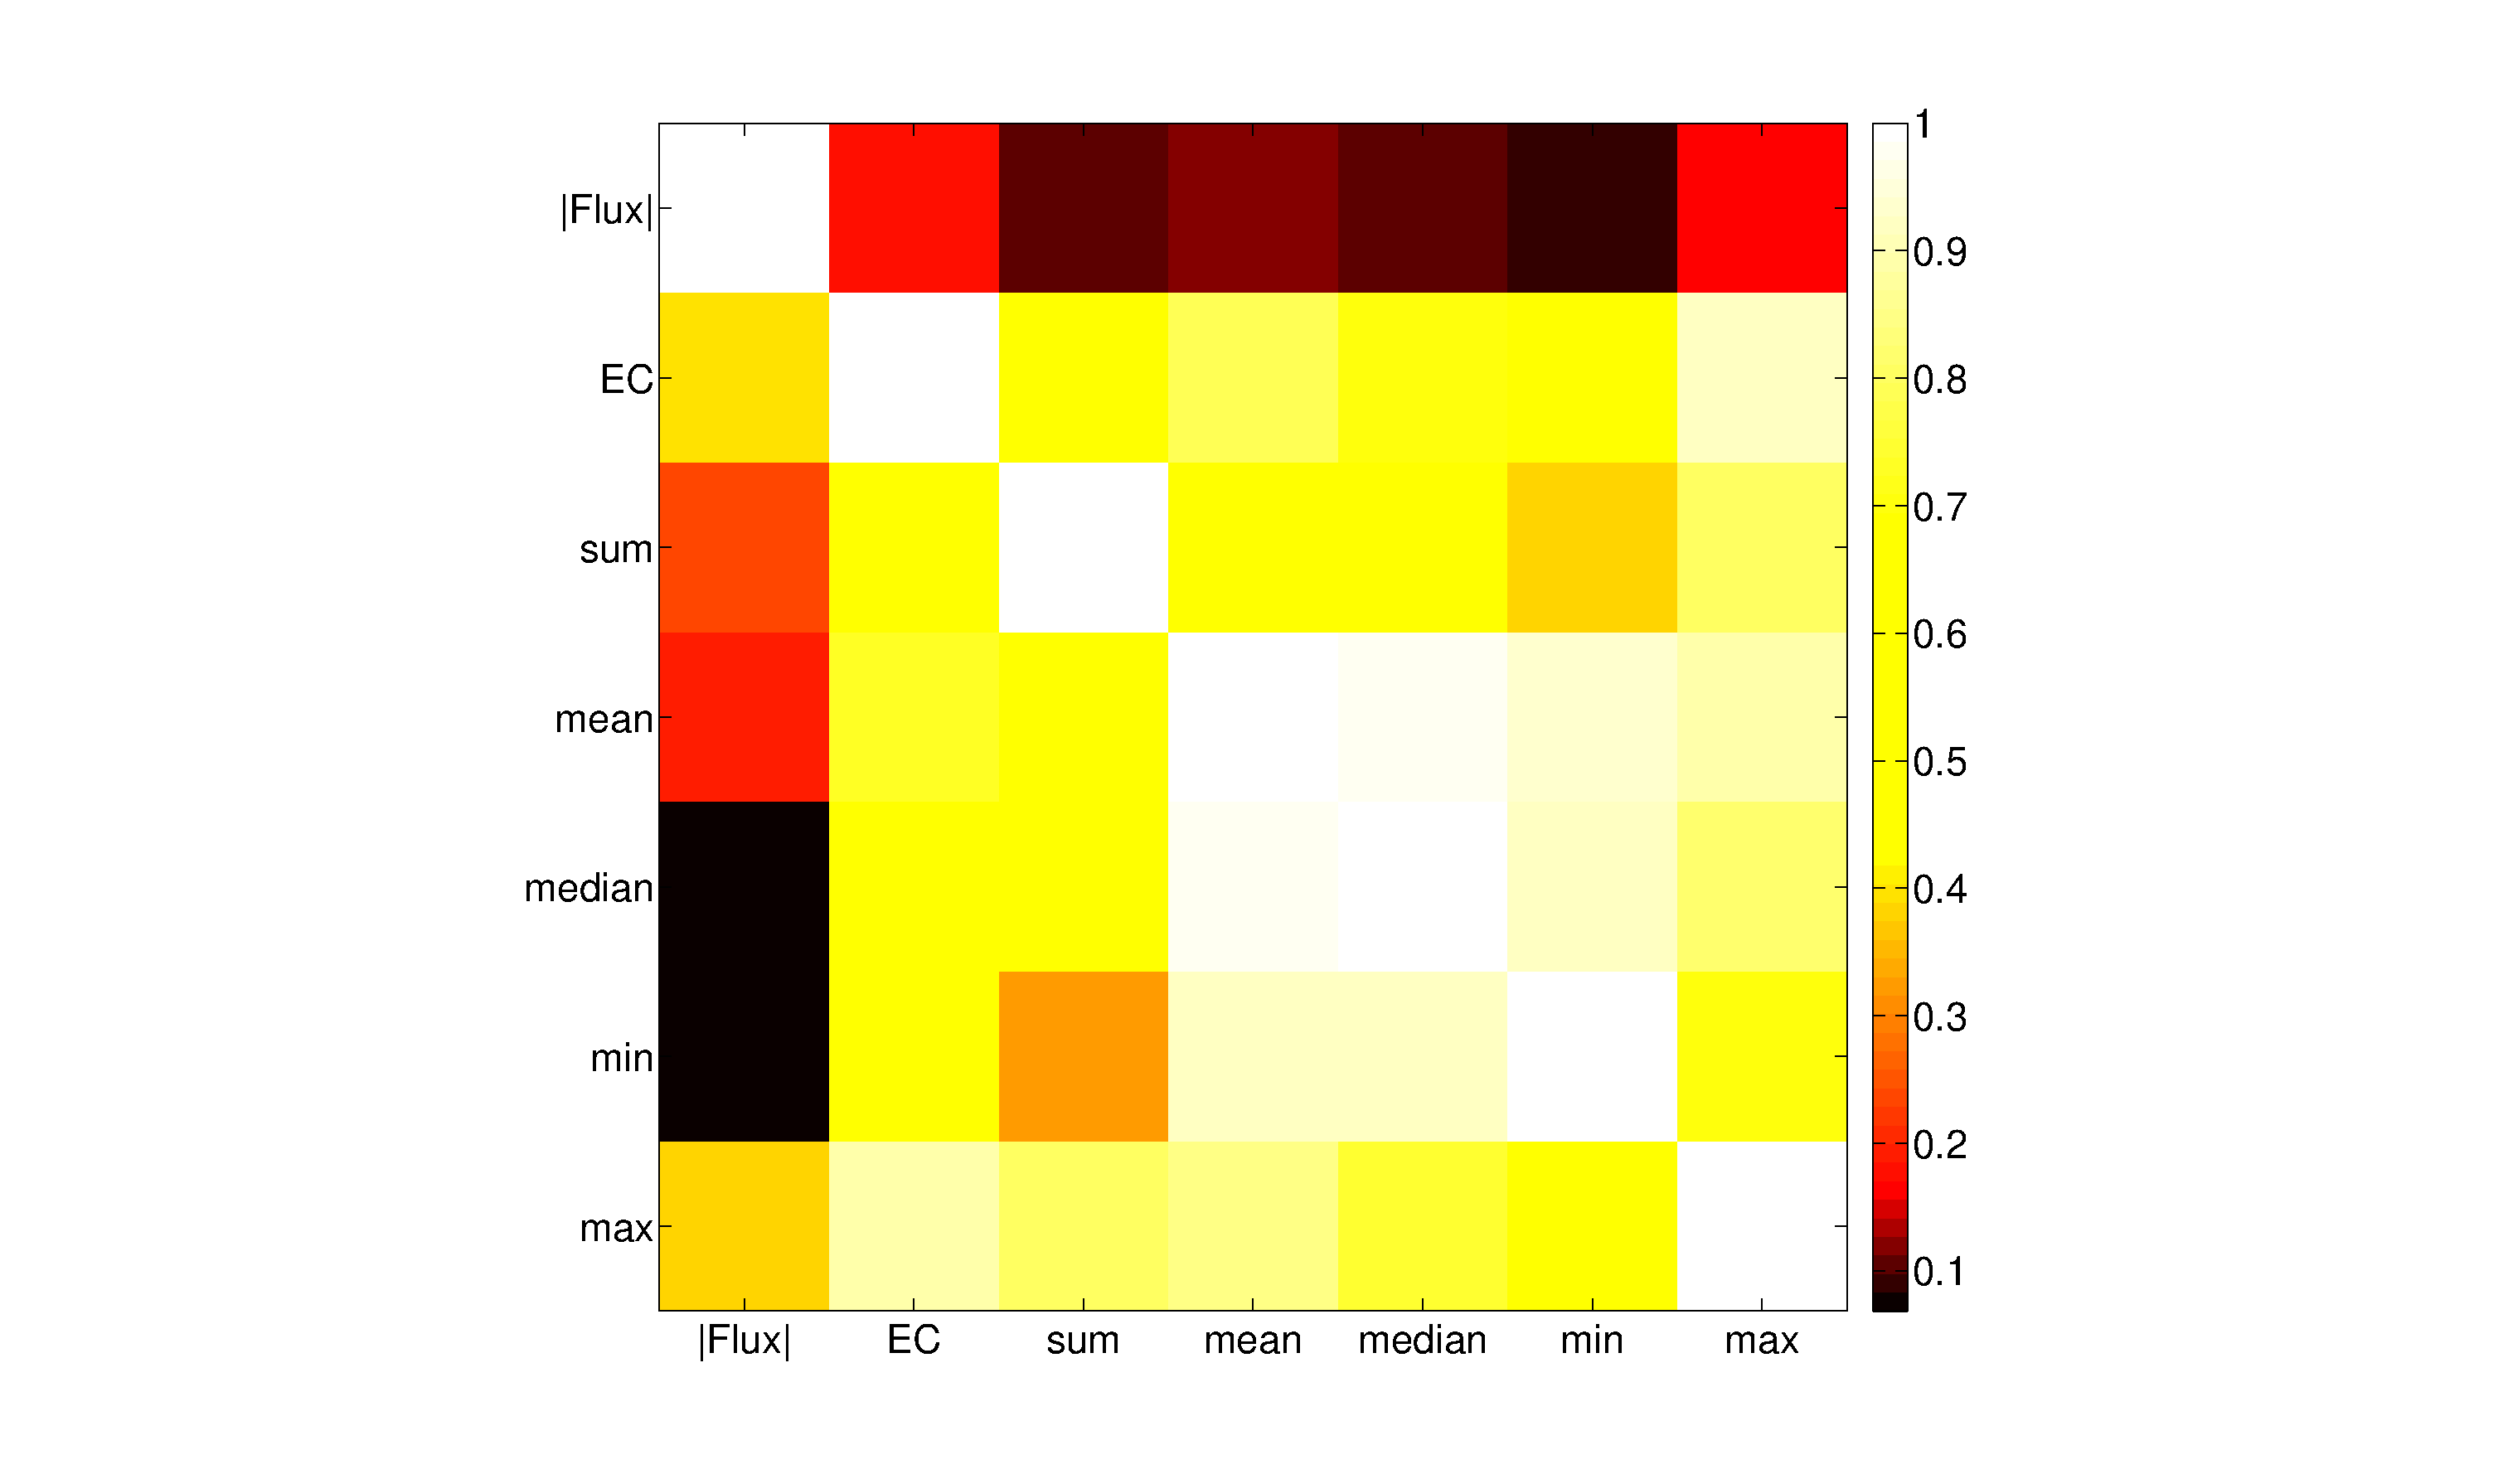
\includegraphics[width=\textwidth, trim=9cm 1.2cm 9cm 1cm, clip=true]
    {HumanExpFluxCompare}
  \caption{human} \label{fig:FluxExpCmp:B}
  \end{subfigure}
\\
\end{tabular}
\caption{Pearson correlation between FALCON flux magnitudes,
prerequisite enzyme complex estimates (from minDisj), and various
simpler gene expression estimates based on the list of genes
associated to each reaction. For yeast \textbf{(a)}, the upper and
lower triangles are the 75\% and 85\% maximum growth conditions,
respectively, and human is done similarly with the K562 and MDA-MB-231
cell lines \textbf{(b)}. As for expression estimates, the sum of
expression and enzyme complex estimate levels are generally the least
correlated with other expression estimates. As expected, the enzyme
complex estimates are the most correlated with the FALCON fluxes, as
they are used in the algorithm. However, it is important to note that
they are not very similar, exemplifying the affect the network
constraints play when determining flux. Interestingly, enzyme complex
abundance is found to correlate very highly with the maximum
expression level for the complex; this can be attributed to many genes
having relatively simple complexes that are isozymes, where one major
isozyme is typically highly expressed.}
\label{fig:FluxExpCmp}
\end{figure}
\FloatBarrier

\section{Assumptions for enzyme complex formation}
\label{sec:complexation}

In order to quantify enzyme complex formation (sometimes called enzyme
complexation), the notion of an enzyme complex should be formalized.
A protein complex typically refers to two or more physically
associated polypeptide chains, which is sometimes called a quaternary
structure. Since we are not exclusively dealing with multiprotein
complexes, we refer to an enzyme complex as being one or more
polypeptide chains that act together to carry out metabolic
catalysis.


\emph{Assumption~\ref{asm:expcorr}.}  A fundamental assumption
that we need in order to guarantee an accurate estimate of (unitless)
enzyme complex abundance are the availability of accurate measurements
of their component subunits. Unfortunately, this is currently not
possible, and we almost always must make do with mRNA measurements,
which may even have some degree of inaccuracy in measuring the mRNA
abundance. What has been seen is that Spearman's $\rho = 0.6$ for
correlation between RNA-Seq and protein intensity in datasets from
HeLa cells \citep{Nagaraj2011}. This implies that much can likely
still be gleamed from analyzing RNA-Seq data, but, an appropriate
degree of caution must be used in interpreting results based on
RNA-Seq data. By incorporating more information, such as metabolic
constraints, we hope to obviate some of the error in estimating
protein intensity from RNA-Seq data.

\emph{Assumption~\ref{asm:isozyme}.} We also include the notion of
isozymes--different proteins that catalyze the same reaction--in our
notion of enzyme complex. Isozymes may arise by having one or more
differing protein isoforms, and even though these isoforms may not be
present in the same complex at the same moment, we consider them to be
part of the enzyme complex since one could be substituted for the
other.

As an example for assumptions described so far, take the $F_1$
subcomplex of ATP Synthase (\Fig~\ref{fig:2F43}), which is composed
of seven protein subunits (distinguished by color, left). On the
right-hand side we see different isoforms depicted as different
colors.  Error in expression data aside, instead of considering the
abundances with multiplicity and dividing their expression values by
their multiplicity, it may be easier to simply note that the axle
peptide (shown in red in the center of the complex) only has one copy
in the complex, so its expression should be an overall good estimation
of the $F_1$ subcomplex abundance. This reasoning will be useful
later in considering why GPR rules may be largely adequate for estimating
the abundance of most enzyme complexes.

\begin{figure*}%[H]
\centering
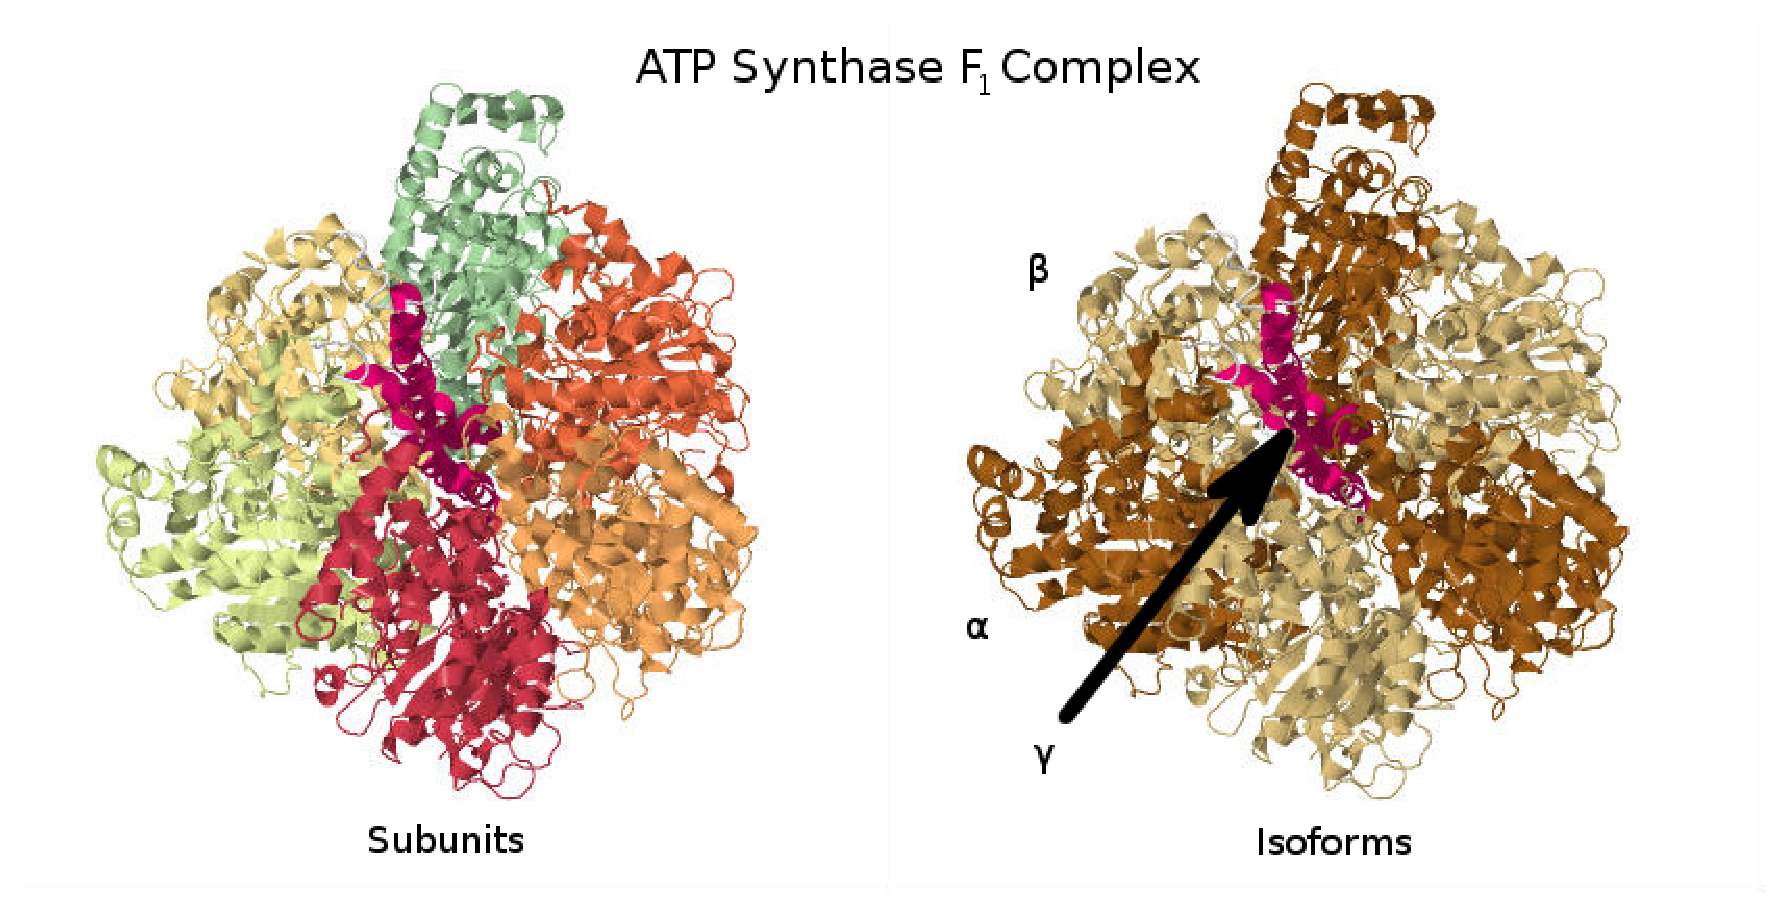
\includegraphics[clip=true,trim=0cm 0cm 0cm 0cm, width=12cm]{2F43}
\caption{Illustration of the $F_1$ part of the ATP Synthase complex
  (PDB ID 1E79; \protect\citealt{Gibbons2000,Bernstein1978,Gezelter}).
  This illustration demonstrates both how an enzyme complex may be
  constituted by multiple subunits (left), and how some of those
  subunits may be products of the same gene and have differing
  stoichiometries within the complex (right).}
\label{fig:2F43}
\end{figure*}

\emph{Assumption~\ref{asm:hierarchy}.}
The modeling of enzyme complex abundance can be tackled by using
nested sets of subcomplexes; each enzyme complex consists of multiple
subcomplexes, unless it is only a single protein or family of protein
isozymes.  These subcomplexes are required for the enzyme complex to
function (AND relationships), and can be thought of as the division of
the complex in to distinct units that each have some necessary
function for the complex, with the exception that we do not keep track
of the multiplicity of subcomplexes within a complex since this
information is, in the current state of affairs, not always known.
However, there may be alternative versions of each functional set
(given by OR relationships). Eventually, this nested embedding
terminates with a single protein or set of peptide isoforms
(e.g.\ isozymes).  In the case of ATP Synthase, one of its functional
sets is represented by the $F_1$ subcomplex. The $F_1$ subcomplex
itself can be viewed as having two immediate subcomplexes: the single
$\gamma$ (axle) subunit and three identical subcomplexes each made of
an $\alpha$ and $\beta$ subunit. Each $\alpha\beta$ pair works
together to bind ADP and catalyze the reaction \citep{Oster2003}. The
$\alpha\beta$ subcomplex itself then has two subcomplexes composed of
just an $\alpha$ subunit on the one hand and the $\beta$ subunit on
the other.  It is obvious that one of these base-level functional
subcomplexes (in this example, either $\gamma$ or $\alpha\beta$) will
be in most limited supply, and that it will best represent the overall
enzyme complex abundance (discounting the issues of multiplicity for
$\alpha\beta$, discussed above).

%
% Consider adding this as a Theorem/Proof:
%

The hierarchical structure just described, when written out in
Boolean, will give a rule in CNF (conjunctive normal form), or more
specifically (owing to the lack of negations), clausal normal form,
where a clause is a disjunction of literals (genes). This is because all
relations are ANDs (conjunctions), except possibly at the inner-most
subcomplexes that have alternative isoforms, which are expressed as
ORs (disjunctions). Since GPR rules alone only specify the
requirements for enzyme complex formation, we will see that not all
forms of Boolean rules are equally useful in evaluating the enzyme
complex abundance, but we have established the assumptions in \suppOrApp
Table~\ref{tab:ECAssume} and an alternative and logically equivalent rule
\citep{Russell2009} under which we can estimate enzyme complex copy
number.

\begin{table}
\def \ECAssumeCap {Assumptions in GPR-based Enzyme Complex Formation}
%\ifthenelse{\boolean{thesisStyle}}{
  \begin{center} % also adds a little needed vspace
  \begin{tabular}{| p{0.9\textwidth} |}
  \hline
  \textbf{\suppOrApp Table~\ref{tab:ECAssume}. \ECAssumeCap} \\
  \hline
  \input{\commonDir falcon_assumptions}
  \\ \hline
  \end{tabular}
  \end{center}

% } {
%   % For Bioinformatics:
%   %\begin{table*}[!t]
%   \processtable{\ECAssumeCap \label{tab:ECAssume}}{
%   \begin{tabular}{| p{\textwidth} |}
%   \hline
%   % I put this in to a separate file because formatting the table in different ways
% is difficult; it may even be better to have multiple versions of this table
% for different documents, but hopefully we can avoid such code duplication.

%Internal part of the table:

\begin{enumerate}
% This is really not related to GPR rules: 
%\ifthenelse{\boolean{thesisStyle}}{\item} {} \label{asm:mm}
%Fluxes in general strive to operate near the $V_{max}$ of the
%reaction, which is proportional to enzyme complex abundance.
\item \label{asm:expcorr}
Expression values are highly correlated with the copy numbers of their
corresponding peptide isoforms.
\item \label{asm:isozyme} 
Protein isoforms contributing to isozymes are considered part of the
same enzyme complex.
\item \label{asm:hierarchy}
Any enzyme complex can be described as a hierarchical subset of
(possibly redundant) subcomplexes; redundant subcomplexes, as
elaborated in (\ref{asm:nostoich}), are not currently modeled.
\item \label{asm:nostoich} 
Assume one copy of peptide per complex; exact isoform stoichiometry
is not considered.
\item \label{asm:sharing} 
With the exception of complexes having identical rules (i.e. the same
complex listed for different reactions), each copy of a peptide
is available for all complexes in the model.
\item \label{asm:active_site}
There is only one active site per enzyme complex.
\item \label{asm:enzyme_sensitivity} 
We assume that different pathways have similar flux sensitivities
with respect to their enzyme abundances.
\item \label{asm:holo} 
If a particular subcomplex can be catalyzed by A and it can also be
catalyzed by A and B (e.g. B acts as a regulatory unit, as in
holoenzymes), this just simplifies to A once expression values are
substituted in. Similarly, allosteric regulation is not
modeled. Relatedly, there are no NOT operations in GPR rules (just ANDs
and ORs).
\item \label{asm:chap} 
Enzyme complexes form without the assistance of protein chaperones and
formation is not coupled to other reactions.
\item \label{asm:posttrans}
Post-translational modifications do not affect complex formation.
\item \label{asm:rate} 
Rate of formation and degradation of complexes doesn't play a role,
since we assume steady-state. 
\end{enumerate}

%   \\ \hline
%   \end{tabular}
%   }
%   {} % caption
% }
\caption{A list of assumptions about how Gene-Protein-Reaction rules 
can describe enzyme complex stoichiometry.}
\label{tab:ECAssume}
\end{table}

There is no guarantee that a GPR rule has been written down with this
hierarchical structure in mind, though it is likely the case much of
the time as it is a natural way to model complexes.  However, any GPR
rule can be interpreted in the context of this hierarchical view due
to the existence of a logically equivalent CNF rule for any non-CNF
rule, and it is obvious that logical equivalence is all that is
required to check for enzyme complex formation when exact isoform
stoichiometry is unknown.  As an example, we consider another common
formulation for GPR rules, and a way to think about enzyme
structure---disjunctive normal form (DNF).  A DNF rule is a
disjunctive list of conjunctions of peptide isoforms, where each
conjunction is some variation of the enzyme complex due to
substituting in different isoforms for some of the required
subunits. A rule with a more complicated structure and compatible
isoforms across subcomplexes may be written more succinctly in CNF,
whereas a rule with only very few alternatives derived from isoform
variants may be represented clearly with DNF.  In rare cases, it is
possible that a GPR rule is written in neither DNF or CNF, perhaps
because neither of these two alternatives above are strictly the case,
and some other rule is more succinct.

\emph{Assumptions~\ref{asm:nostoich},~\ref{asm:sharing}~and~\ref{asm:active_site}.}
One active site per enzyme complex implies a single complex can only
catalyze one reaction at a time. Multimeric complexes with one active
site per identical subunit would be considered as one enzyme complex
per subunit in this model. Note that it is possible for an enzyme
complex to catalyze different reactions. In fact, some transporter
complexes can transfer many different metabolites across a lipid
bilayer---up to 294 distinct reactions in the reversible model for
solute carrier family 7 (Gene ID 9057).  Another example is the
ligation or hydrolysis of nucleotide, fatty acid, or peptide chains,
where chains of different length may all be substrates or products of
the same enzyme complex. While we do not explicitly consider these in
in the minimum disjunction algorithm, these redundancies are taken into
account subsequently in Algorithm~\ref{alg:FALCON}.

What is currently not considered in our process is that some peptide
isoforms may find use in completely different complexes, and in some
cases, individual peptides may have multiple active sites; in the
first case, we assume an unrealistic case of superposition where the
isoform can simultaneously function in more than one complex. The
primary reason we have not tackled this problem is because exact
subunit stoichiometry of most enzyme complexes is not accurately
known, but an increasing abundance of data on BRENDA
\citep{Schomburg2013} gives some hope to this problem. A recent
\textit{E. coli} metabolic model incorporating the metabolism of all
known gene products \citep{O'Brien2013} also includes putative
enzyme complex stoichiometry in GPR rules. For the second point, there
are a few enzymes where a single polypeptide may have multiple active
sites (e.g.\ fatty acid synthase), and this is not currently taken into
account in our model. 

\emph{Assumption~\ref{asm:holo}.}
We do not make any special assumptions requiring symmetry of an
isoform within a complex. For instance, the example in
assumption~\ref{asm:holo} shows how you might have one subcomponent
composed of a single isoform, and another subcomponent composed of
that gene in addition to another isoform. In this case, it is simply
reduced to being the first gene only that is required, since clearly
the second is strictly optional. That isn't to say that the second
gene may not have some metabolic effect, such as (potentially) aiding in
structural ability or altering the catalytic rate, but it should have
no bearing on the formation of a functional catalytic
complex. Holoenzymes---enzymes with metabolic cofactors or protein
subunits that have a regulatory function for the complex---would
likely be the only situation where this type of rule might need to be
considered in more detail. But in the absence of detailed kinetic
information, this consideration (much like allosteric
regulation) is not useful.

No additional algorithmic considerations are needed, as this is a
by-product of the conversion to CNF. For instance, take the following
example where the second conjunction has the redundant gene $g_3$: 

\[(g_1 \land g_2) \lor (g_1 \land g_2 \land g_3)\]

Distributing during the process of conversion to CNF results in:

\[
g_1 \land (g_1 \lor g_2 ) \land (g_1 \lor g_3) \land (g_2 \lor g_1) 
\land g_2 \land (g_2 \lor g_3)
\]

Because every disjunction with more than one literal is in conjunction
with another disjunction with only one of its literals, the
disjunction with fewer literals will be the minimum of the two once
evaluated. This applies to both of the singleton disjunctions $g_1$
and $g_2$, so all other disjunctions will effectively be ignored (it
is up to the implementer whether the redundant sub-expressions are
removed before evaluation):

\[
g_1 \land \bcancel{(g_1 \lor g_2 ) \land} \bcancel{(g_1 \lor g_3) \land} 
\bcancel{(g_2 \lor g_1) \land} g_2 \bcancel{\land (g_2 \lor g_3)} 
= (g_1 \land g_2)
\]


\emph{Assumption~\ref{asm:enzyme_sensitivity}.}
Another important biochemical assumption is that reactions should
operate in a regime where they are sensitive to changes in the overall
enzyme level in the pathways that they belong in
\citep{Bennett2009,Chubukov2013}. This is perhaps the most important
issue to be explored further for methods like this, since if it is not
true, some other adjustment factor would be needed to make the method
realistic. For instance, if all reactions in a pathway are operating
far below $V_{max}$, but it is not the case in another pathway, the
current method does not have information on this, and will try to put
more flux through the first pathway than should be the case.

\emph{Assumptions~\ref{asm:chap}~and~\ref{asm:rate}.}
Due to the quickness, stability, and energetic favorability of enzyme
complex formation, the absence of chaperones or coupled metabolic
reactions required for complex formation may be reasonable
assumptions, but further research is warranted \citep{Karr2012}.
Additionally, as in metabolism, we assume a steady state for complex
formation, so that rate laws regarding complex formation aren't
needed. However, further research may be warranted to investigate the
use of a penalty for complex levels based on mass action and
protein-docking information. Requisite to this would be addressing
assumption~\ref{asm:nostoich}. It would be surprising (but not
impossible) if such a penalty were very large due to the cost this
would imply for many of the large and important enzyme complexes
present in all organisms \citep{Nelson2008}.

\clearpage

\section{Benchmarking of solvers}
We have exclusively used the Gurobi solver \citep{gurobi} for this
work, which is a highly competitive solver that employs by default a
parallel strategy to solving problems: a different algorithm is run
simultaneously, and as soon as one algorithm finished the others
terminate. Of course, if there is a clear choice of algorithm for a
particular problem class, this should be used in production settings
to avoid wasted CPU time and memory. In order to address this, we
benchmarked the three non-parallel solver methods in Gurobi
 (since parallel solvers simply use multiple methods simultaneously).
The exception to this rule is the Barrier method, which can use
multiple threads, but in practice for our models appears to use
no more than about 6 full CPU cores simultaneously for our models.
Our results for Yeast~5 and Yeast~7 with minimal directionality constraints
\citep{Heavner2012,Lee2012,Aung2013} and Human Recon~2 \citep{Thiele2013}
are shown in \suppOrApp Table~\ref{tab:methodTime}).

\begin{table}
\begin{center}
\begin{tabular}{rrrr}
\emph{Model}                 & \emph{Primal-Simplex} & \emph{Dual-Simplex} & \emph{Barrier} \\
Yeast~5.21 (2,061 reactions) & $ 7.841 \pm 1.697    $ & $ 7.611 \pm 1.267    $ & $ 10.859 \pm 2.788   $\\ 
Yeast~7.0 (3,498 reactions)  & $ 51.863 \pm 22.731  $ & $ 65.317 \pm 12.771  $ & $ 242.137 \pm 57.129 $\\
Human 2.03 (7,440 reactions) & $ 159.077 \pm 24.903 $ & $ 152.297 \pm 39.783 $ & $ 366.166 \pm 92.321 $\\
\end{tabular}
\end{center}
\caption{Running times (in seconds, $\pm$ standard deviation) for
  FALCON using various algorithms implemented in the Gurobi package.
  For yeast models, 1,000 replicates were performed, and for the human
  model, 100 replicates were performed.}
\label{tab:methodTime}
\end{table}

We found that in Yeast~7 with the primal-simplex solver, there is a
chance the solver will fail to find a feasible solution.
We verified that this is a numeric issue
in Gurobi and can be fixed by setting the Gurobi parameter
\texttt{MarkowitzTol} to a larger value (which decreases
time-efficiency but limits the numerical error in the
simplex algorithm). In practice, failure for the algorithm to converge
at an advanced iteration is rare and is not always a major problem (since the previous
flux estimate by the advanced iteration should already be quite good), but it
is certainly undesirable; a warning message will be printed by
\texttt{falcon} if this occurs, at which point parameter settings can
be investigated. In the future, we plan to improve \texttt{falcon} so
that parameters will be adjusted as needed during progression of the
algorithm after finding a good test suite of models and data. For now,
we use the dual-simplex solver, for which we have always had good
results.

Because the number of iterations depends non-trivially on the model
and the expression data, it may be more helpful to look at the 
average time per iteration in the above examples 
(\suppOrApp Table~\ref{tab:methodTimeIter}).

\begin{table}
\begin{center}
\begin{tabular}{rrrr}
\emph{Model}                 & \emph{Primal-Simplex} & \emph{Dual-Simplex} & \emph{Barrier} \\
Yeast~5.21 (2,061 reactions) & $ 0.721 \pm 0.023 $ & $ 0.652 \pm 0.040 $ & $ 1.100 \pm 0.112  $\\ 
Yeast~7.0 (3,498 reactions)  & $ 2.725 \pm 0.298 $ & $ 2.469 \pm 0.289 $ & $ 11.309 \pm 1.589 $\\
Human 2.03 (7,440 reactions) & $ 6.422 \pm 0.484 $ & $ 5.233 \pm 0.661 $ & $ 15.782 \pm 3.209 $\\ 
\end{tabular}
\end{center}
\caption{Running time per FALCON iteration (in seconds, $\pm$ standard
  deviation) using various algorithms implemented in the Gurobi
  package.  For yeast models, 1,000 replicates were performed, and for
  the human model, 100 replicates were performed.}
\label{tab:methodTimeIter}
\end{table}

Given the above rare trouble with primal simplex solver the universal
best performance enjoyed by the dual-simplex method (\suppOrApp Tables
\ref{tab:methodTime} and \ref{tab:methodTimeIter}), we would advise
the dual-simplex algorithms, all else being equal. The dual-simplex
method is also recommended for memory-efficiency by Gurobi
documentation, but we did not observe any differences in memory for
different solver methods.

All timing analyses were performed on a system with four 8-core AMD
Opteron\texttrademark\ 6136 processors operating at 2.4
GHz. \Fig~\ref{fig:FluxBars}, Table~\ref{tab:FalcPerf}, and \suppOrApp
Tables \ref{tab:methodTime} and \ref{tab:methodTimeIter} used a single
unperturbed expression file per species (\textit{S. cerevisiae} and
\textit{H. sapiens}; see \texttt{timingAnalysis.m} for
details). Values were averaged across 32 replicates. \suppOrApp
Note that the iMAT method is formulated as a mixed integer program
\citep{Shlomi2008}, and was able to use additional parallelization of
the solver \citep{gurobi} whereas other methods only used a single
core (our system had 32 cores and iMAT with Gurobi would use all of
them). Tables~\ref{tab:methodTime} and \ref{tab:methodTimeIter} used
multivariate log-normal noise multiplied by the original expression
vector to introduce more variance in the calculations; the human
models were tested with 100 replicates and the yeast models with 500
replicates.

\section{Generation of figures and tables}

All non-trivial figures can be generated using MATLAB scripts found in
the \texttt{analysis/figures} subdirectory of the FALCON installation.
In particular, figures should be generated through the master script
\texttt{makeMethodFigures.m} by calling
\texttt{makeMethodFigures(figName)} where \texttt{figName} has a name
corresponding to the desired figure.  In some cases, some MATLAB
\texttt{.mat} files will need to be generated by other scripts first;
see the plotting scripts or the subsections below for details. An
example is to make the scatter plots showing the difference between
running falcon with enzyme abundances determined by direct evaluation
or the minimum disjunction algorithm; all three scatter plots are
generated with the command \texttt{makeMethodFigures(\textquotesingle
fluxCmpScatter\textquotesingle)}. Note that, as written, this requires
a graphical MATLAB session.

\begin{sloppypar}
Comparison of the effects of the employed enzyme complexation methods
were evaluated using \texttt{compareEnzymeExpression.m} and 
\texttt{compareFluxByRGroup.m}. Comparison of reacion groups was
performed in \texttt{compareFluxByRGroup.m}.
\end{sloppypar}

\subsection{Timing analyses}
All timing analyses were performed on a system with four 8-core AMD
Opteron\texttrademark\ 6136 processors operating at 2.4 GHz. 
\Fig~\ref{fig:FluxBars} and Table~\ref{tab:FalcPerf} used unperturbed
expression data; see
\texttt{yeastResults.m} for details). Values for the FALCON method
were averaged across 32 replicates, while values for the
\citealt{Lee2012} method were averaged across 8 replicates. Human
timing analyses were performed using \texttt{methodTimer.m} with
8 replicates.

\subsection{Data sources}
Enzyme complexation comparisons were performed on proteomics data
from \citealt{Gholami2013} (Human; 786-O cell line) and 
\citealt{Picotti2013} (yeast; BY strain), and on RNA-Seq data
from \citealt{Lee2012} (yeast; 75\% max $\mu$ condition).